\chapter{Data Analysis I: Calibration and Corrections}

Need to explain pedestal subtraction 
GG noise subtraction 

\section{Software}
\label{sec:software}

The S$\pi$RITROOT software is modular tasked based code based on the FAIRROOT package written in C++ \cite{fairroot}. The main tasks in the S$\pi$RITROOT software reconstruction are:
\begin{itemize}
  \item Decoder task
  \item Pulse Shape Algorithm (PSA Task)
  \item Helix Track Finding Algorithm
  \item Clustering Algorithm
  \item Track Fitting (GENFIT package)
  \item Vertex Fitting (RAVE package)
\end{itemize}

The decoder task converts the binary data file into a container class which maps the electronics channels into the corresponding pads and (x,z) coordinates. 

There may be several pulses in a pad coming from two tracks passing under the same pad separated  by arrival time. Using an expected pulse shape the PSA task fits the signal pulses within a pad, giving the arrival time of the drifted electrons from each particular track. The height of the fitted pulse is proportional to the total charge of that event, Q and the y-coordinate is calculated as $y = v\cdot t_0$ where $v$ is the drift velocity and $t_0$ the arrival time. Combining the information from these first two tasks, (x,y,z,Q), we construct what is called a "hit". 

 The Helix Track Finding Algorithm finds the collection of hits belonging to one track out of all the hits in an event. The hits within a track are then reduced into clusters. A cluster's position is the average position of the hits within a cluster, with the total charge of the cluster being the sum of the hits charges. 
 
 A tracks average position is estimated by the cluster's average position. The clusters are then fitted in the GENFIT track fitting package \cite{genfit}, giving the final momentum of the track. A final vertex of the event is fitted from all tracks using the package RAVE \cite{rave}. 

\paragraph{Definition of clustering}

A brief description of the method of clustering is illustrated in Figure \ref{fig:topview}. It is impractical to cluster in both the x and z-axis and we only cluster the hits along one axis. The three clusters at the bottom of Figure \ref{fig:topview} are clustered along the x-axis and the upper three are along the z-axis, as shown by the bolded pads for one of the clusters in each direction.

 The clustering direction depends on the angle  of the track with respects to the x-axis, defined as $\theta$. For example, a track going along the z-axis the crossing angle is defined as $90^{\circ}$, and a track going along the x-axis defined as $0^{\circ}$. In the case that the crossing angle is $45^{\circ} < \theta \leq 90^{\circ} $ the clustering direction is along the x-axis. For $0^{\circ} < \theta \leq 45^{\circ}$ it is along the z-axis. 

 The position along the clustering direction is calculated by weighting the individual hit's positions by their charges $q_i$ and getting the mean value. The other direction is set to the center of the pad. For example if we are clustering along the x-axis for a cluster, the z-position is set to the center of the pad in the z-direction and vice versa. 

Clustering in this way gives us better position resolution for calculating the position of each cluster. You could imagine if we calculated the clusters only along the x-axis for tracks with $\theta \approx 0^{\circ}$ the x-position is not well defined. By clustering in the direction most perpendicular to the track, we get a better position resolution.

\begin{figure}[H]
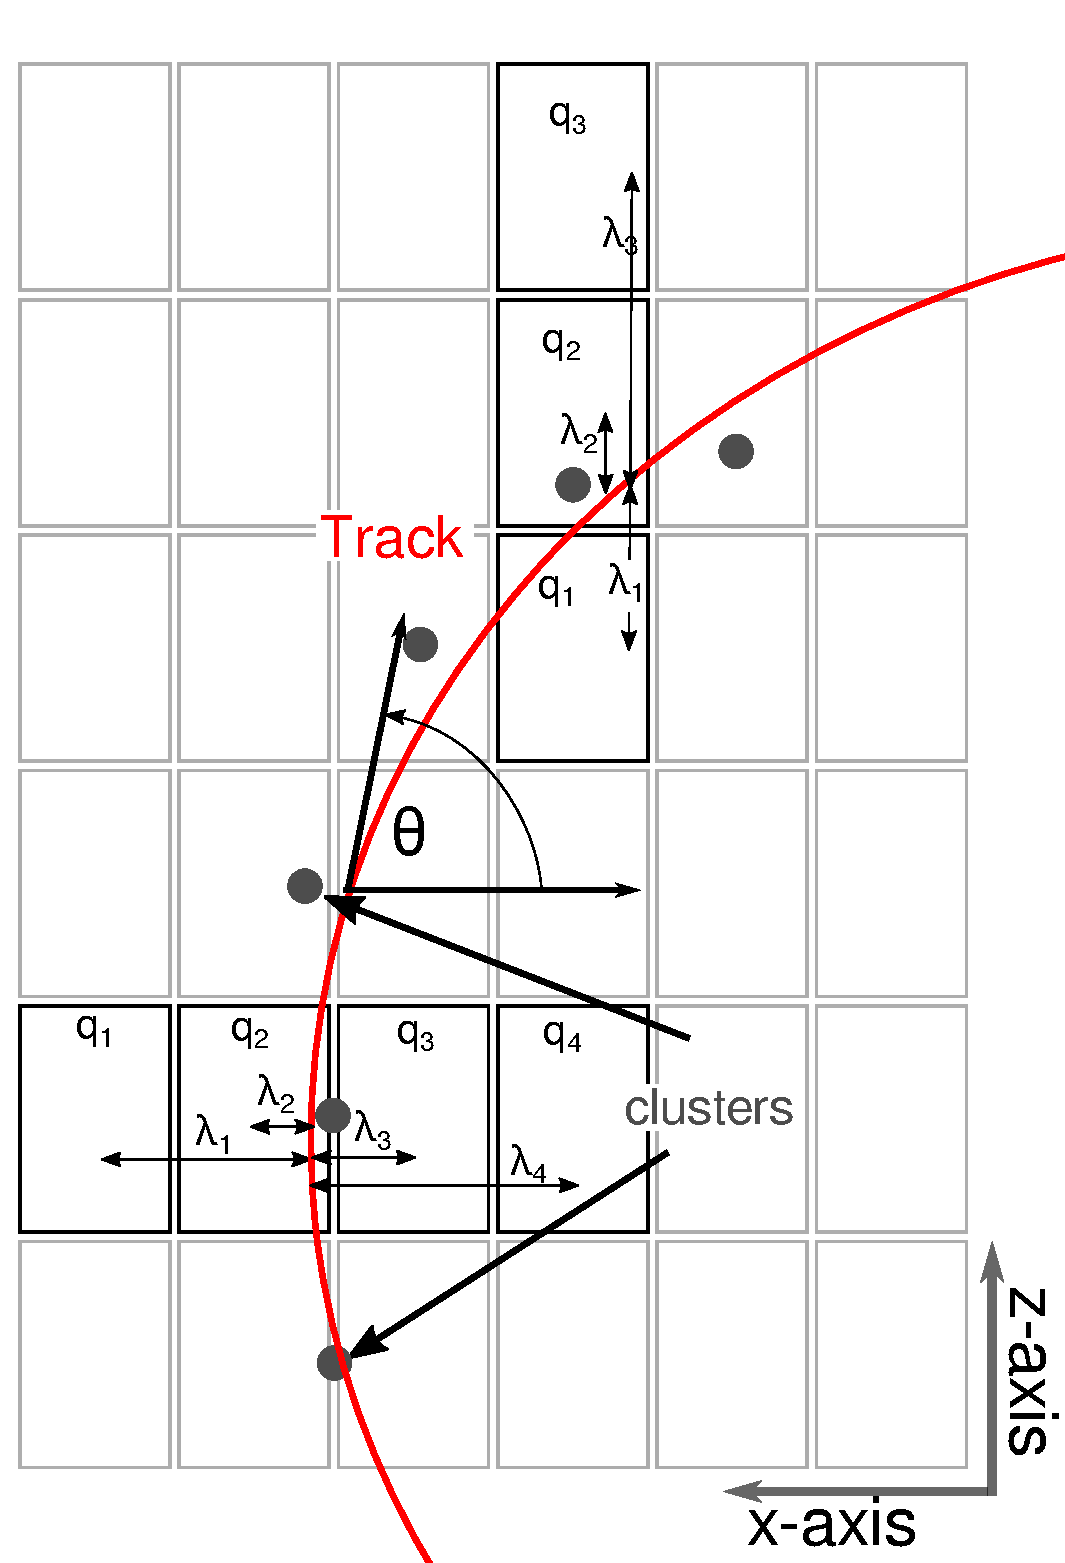
\includegraphics[scale=.5]{top_view_helix_ext.pdf}
\caption{Cartoon graphic of a top down view of a fit to a track passing through several pads. The bolded pads and the charges $q_i$ represent the hits belonging to that pad and the clusters of the track representing the average position of the track. The three clusters at the bottom are clustered in the x-direction and for the upper three clustered in the z-direction. The estimate of the position of the avalanche is given by the track fit and the position from the center to each pad to the $\bar{x}$ position is given as $\lambda_i$.}
\label{fig:topview}
\end{figure}


\subsection{Pulse Shape Algorithm}
\label{sec:psa}

\section{Calibrations and Corrections}


\subsection{Cocktail calibration}

\begin{table*}\centering
\ra{1.3}
\begin{tabular}{@{}rrrrrrr@{}}\toprule
& \multicolumn{3}{c}{$100 MeV Target$}\\
\cmidrule{2-4}
Particle &\phantom{abc} & Measured & Corrected & \% Difference & \% Difference\\
\midrule
p   & 882.8 & 929.5 & 877.3   &  3.7  & -1.0  \\
d   & 817.1 & 831.15 & 797.94 &  1.7  & -2.3\\
\bottomrule
\end{tabular}
\caption{Summary of expected cocktail. }
\label{tb:cocktail100tar}
\end{table*}

\begin{table*}\centering
\ra{1.3}
\begin{tabular}{@{}rrrrrrr@{}}\toprule
& \multicolumn{3}{c}{$100 MeV$}\\
\cmidrule{2-4}
Particle & Expected & Measured & Corrected & \% Difference & \% Difference\\
\midrule
p   & 882.8 & 903.5 & 889   &  2.0   & -1.6  \\
d   & 817.1 & 898.5 & 874.5 &  2.1   & -2.7\\
\bottomrule
\end{tabular}
\caption{Summary of expected cocktail. }
\label{tb:cocktail100}
\end{table*}

\begin{table*}\centering
\ra{1.3}
\begin{tabular}{@{}rrrrrrr@{}}\toprule
& \multicolumn{3}{c}{$300 MeV$}\\
\cmidrule{2-4}
Particle & Expected & Measured & Corrected & \% Difference Raw & \% Difference Corrected\\
\midrule
d   & 1621 & 1704 & 1612   &  5.1 & -0.6  \\
t   & 1612 & 1691 & 1596   &  4.9  & -1.0\\
${}^{4}$He   & 1613 & 1698 &  5.3 & 1595  & -1.1\\

\bottomrule
\end{tabular}
\caption{Summary of expected cocktail. }
\label{tb:cocktail300}
\end{table*}


\begin{table*}\centering
\ra{1.3}
\begin{tabular}{@{}rrrrcrrrcrrr@{}}\toprule
& \multicolumn{3}{c}{$100 MeV$} & \multicolumn{3}{c}{$100 MeV$} & \multicolumn{3}{c}{$300 MeV$}\\
\cmidrule{2-4} \cmidrule{6-8} \cmidrule{10-12}
& &\multicolumn{2}{c}{Measured} & & \multicolumn{2}{c}{Measured} & & \multicolumn{2}{c}{Measured}\\
\cmidrule{3-4} \cmidrule{7-8} \cmidrule{11-12}
Particle &\phantom{abc} & Measured & E$\times$B\\
\midrule
p   & 882.8 & 929.5 & 877.3 & 903.5 & 929.5 & 889 &\phantom{abcdef} & f & f \\
d   & 817.1 & 831.15 & d & 898.5 & e & e & 1621.1 & 1704 & 1612\\
t   & 589.5 & d & d & 887 & e & e & 1612.4 & f & f  \\
$^{3}$He  & 1617.3  & d & d & 1795.2 & e & e & 3236.4 & f & f\\
$^{4}$He  & 1405.6  & d & d & 1782.9 & e & e & 3226.4 & f & f \\
\bottomrule
\end{tabular}
\caption{Summary of expected cocktail. }
\label{tb:cocktailsummary}
\end{table*}

Light charged particles (p,d,t,${}^{3}$He,${}^{4}$He), beams were produced and measured in the TPC. The magnetic and slit settings of the dipoles in the BIGRIPS spectrometer was set so that the measured momentum resolution of the beam was $\frac{\delta p}{p}$ < 1\%. Two magnetic rigidity settings were studied, with an empty target. A thick Aluminum target was used to provide a slightly lower point for part of the lower rigidity setting, effectively creating three calibration points over several particle species. The production of certain particles (t,${}^{3}$He), produced too few counts to make a good measurement, and in the high momentum rigidity setting protons could not propagate down the line and there were no counts. 

Since the expected momentum resolution resulting from the spectrometer was less than 1\%, the observed momentum resolution measured by the TPC is a good measurement of the combined momentum resolution of the software and TPC (intrinsic detection) system. The momentum resolution of the TPC depends on several factors such as the particle's angle, momentum, charge, track multiplicity, etc. This calibration beam represents and ideal situation where the track was parallel to the pad plane and only one particle was measured at one time. The energy loss resolution can also be directly inferred from the measurement since each energy setting represents a monochromatic source of each particle species, which has a well defined energy loss distribution. An average momentum resolution of ~2\% and the energy loss resolution of ~ 5\% was measured for particles ranging from protons to ${}^{4}$He, over the range of momenta measured in the calibration beam as summarized in Table~\ref{tb:momresolution}.

Since magnetic dipole setting of the BIGRIPS spectrometer define the energy of each particle type we can calculate the expected momenta of each particle species measured. Small corrections to the momenta were propagated using LISE++ software which can calculate the energy loss through several materials in the beam line. These corrections resulted in a small change in the momenta. The measured momenta of the calibration beam differed significantly from the expected values as seen in Tables~\cref{tb:cocktail100tar,tb:cocktail100,tb:cocktail300}. This effect is attributed to inhomogenatities in the magnetic field which introduces electron drift velocity in the direction of $\vec{E}\times\vec{B}$ direction. The $\vec{E}\times\vec{B}$ dift velocity causes the electron trajectories to shift toward the +x-axis in the TPC coordinates causing particles of positive charge (going in the -x-axis) to have a higher measured momenta than in reality. The disagreement in measured and expected momenta is upwards of ~5\% difference in the higher momentum calibration settings. The details of the correction technique are discussed in the later Section~\ref{sec:spacecharge} are discussed in a more general correction which also includes correction for the space charge; the same correction technique was applied here in the special case of zero space charge which is the special case of only having $\vec{E}\times\vec{B}$ components .

The values under the corrected column of seen in Tables~\cref{tb:cocktail100tar,tb:cocktail100,tb:cocktail300}, represent the data correcting for $\vec{E}\times\vec{B}$. A significant improvement is seen in the high momentum setting going from around ~5\% disagreement to within ~1\% agreement in the corrected data. For the lower momentum settings (Tables~\cref{tb:cocktail100tar,tb:cocktail100}), protons see a slight improvement of about ~1\% where as the deuterons are over corrected in both settings. The level of agreement of the all corrected values is still within the estimated momentum resolution of the TPC. 

\begin{table*}\centering
\ra{1.3}
\begin{tabular}{@{}rr@{}}\toprule
Momentum Resolution \% & <dE/dx> Resolution \% \\
\midrule
1.6  & 4.6\\
\bottomrule
\end{tabular}
\caption{Summary of expected cocktail. }
\label{tb:momresolution}
\end{table*}

Picture of cocktail before and after ExB effect
Table of LISE++ expected cocktail energies ridigity setting of dipole magnets (reference big rips line)



\subsection{Electronics calibration}
The channel number of the electronics was calibrated by measuring the response of each channel to an input pulse supplied by a pulse generator. The pulse was injected into the ground plane of the TPC. This distributed the pulse evenly across the entire pad plane over a range of input voltages. The input voltage is plotted as a function of the measured ADC channel in Fig.~\ref{fig:gaincalib} for every channel. The small variation in each channel can be seen as the wide band around each measurement point. A linear fit is performed to get the best fit line which provides a reference line which each channel is calibrated to. The right panel shows the resulting distribution of channels after calibration. This is a relative calibration technique meant to calibrate the varying gains in each channel relative to one another. 

\begin{figure}[H]
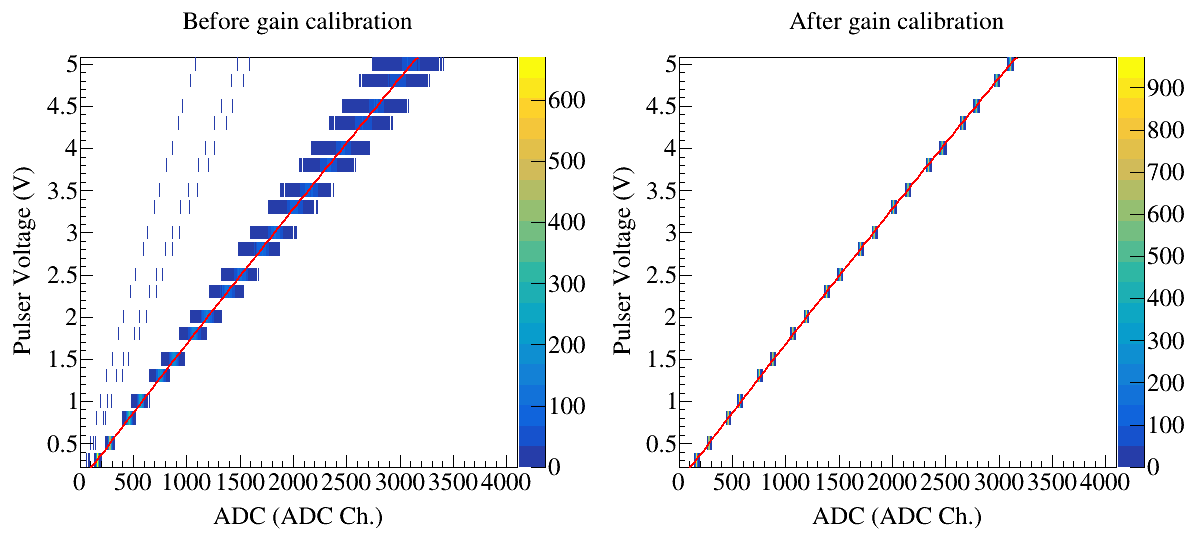
\includegraphics[width=\linewidth]{gaincalib.png}
\caption{Calibration of electronics}
\label{fig:gaincalib}
\end{figure}

\subsection{Anode gain calibration}

As mentioned earlier, the anode wires were separated into 14 independently biased sections. The high voltage of sections 12 and 14 were reduced during the experiment due to high currents being observed on the wires. The wire section voltages were lowered once and adjusted once again. Out of all the runs used in the analysis in this thesis \ref{tb:runList}, the anode sections 12 and 14 were lowered to \SI{1085}{\volt} for runs 2272-2371 and set to \SI{1214}{\volt} for all the other runs. By lowering the voltage on these anode wires, the gas gain is lowered as compared with all the other anode wire plane sections which operate at \SI{1460}{\volt}. To account for the drop in gain, in the software we increase the gain of the pads which lie above these anode wires. To calibrate these sections we perform a relative calibration to the high gain anode sections by comparing the energy loss values of the high and low gain sections. 


\begin{figure}[H]
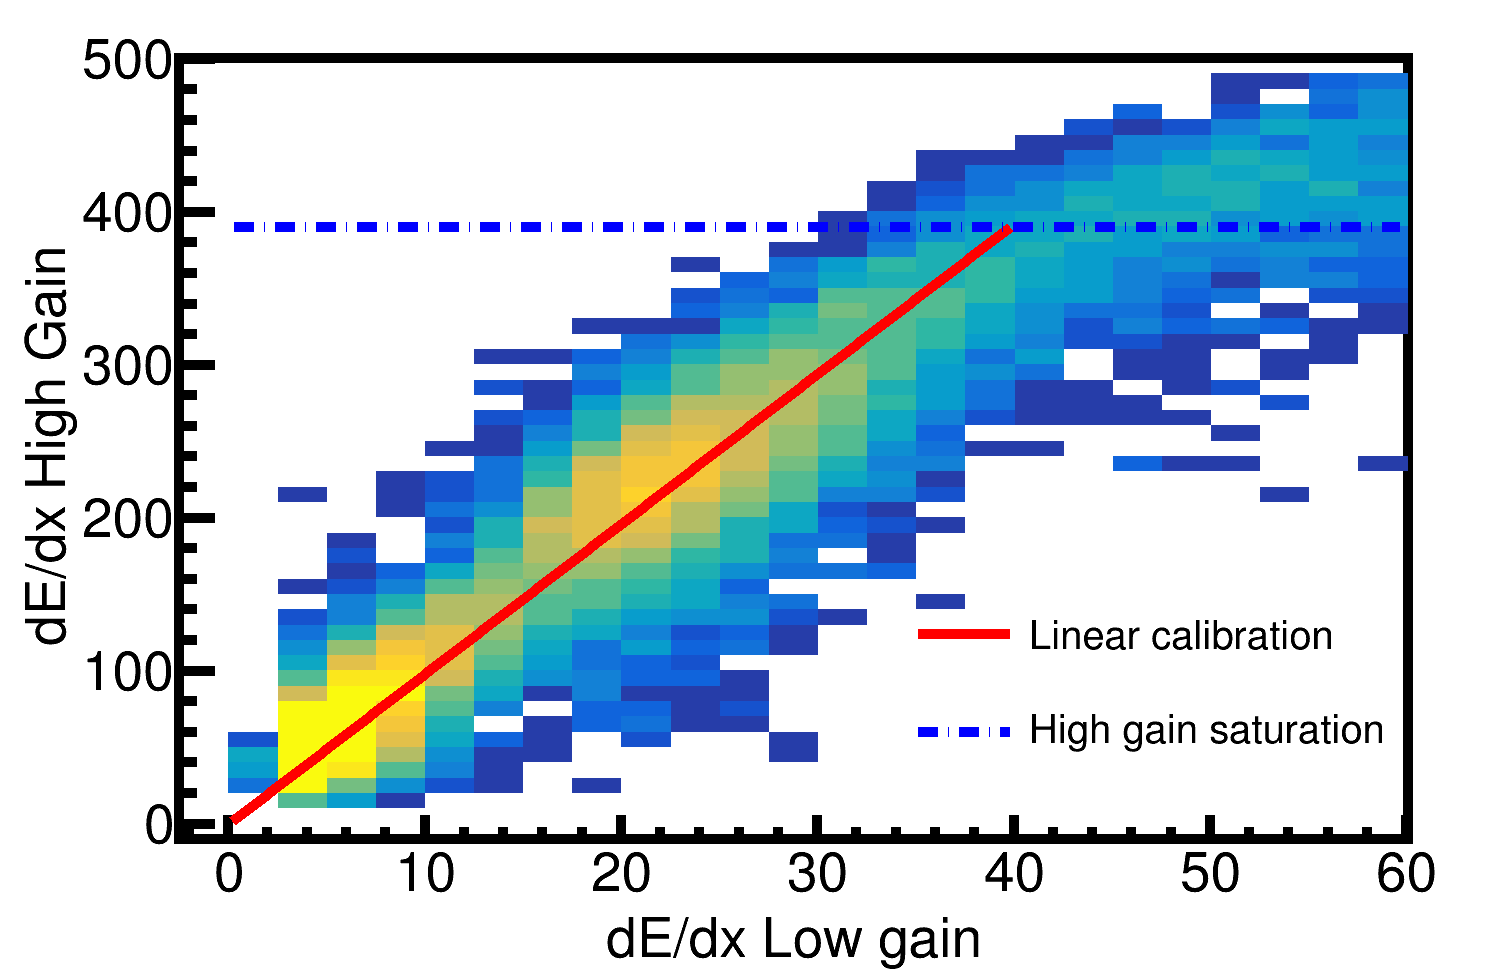
\includegraphics[width=\linewidth]{highlowcal.png}
\caption{Calibration of low high.}
\label{fig:highlowcal}
\end{figure}


\subsection{Extending the dynamic range of the Electronics}
Using a TPC for measurements of HIC in nuclear physics presents a different set of challenges as opposed to higher energy experiments. Typically in higher energy experiments the charge of particles is Z$e$, where Z=1. Also the particles are traveling at higher energies in which the energy losses in a detector range from the minimum of the energy loss curve to the small logarithmic climb CITE FIGURE HERE!!!. The dynamic range of electronics in such experiments can cover a wide range of particle energies in the energy loss curve. In nuclear HICs, we are interested in cluster of nucleons typically from Z=1-3 resulting from the collision, and even higher in some applications. As seen in Eq.~\ref{eq:bb}, the energy loss is proportional to $Z^2$; the energy values of the resulting particles are at much lower energies which are in the $1/\beta^2$ region. The energy range and particle types covered by the electronics are significantly limited as they quickly reach the dynamic range limitations of the electronics as the charge of a particle increases and the velocity decreases. 

Several TPCs have tried to address this issue by having regions of low and high gain, either in amplification gain or in electronics gain. Here we run into the issue that high velocity particles will have little to no signal in the low gain regions. At lower velocities, particles will deposit much charge over the low gain regions but will saturate the high gain regions, whose charge values are usually lost. Only within the dynamic range will tracks have the best momentum resolution, outside the dynamic range clusters will be missing in the sections which depend on the track velocity, lowering the momentum resolution of tracking. There are ongoing efforts in the nuclear community to develop new electronics which hope to mitigate these persistent issues in TPC electronics CITE HERE, by being able to switch to a lower gain value when the maximum range is reached. Though, it is quite useful to develop a software technique which may extend the dynamic range of TPC electronics without the use of external hardware, espeically in experiments which have already been performed with older electronics technologies. 

In TPCs, the effective dynamic range can be very different from the single pad dynamic range. Typically TPCs are operated inside of a magnetic field for reconstructing momentum of each particle, which requires sub-millimeter precision in the position determination of the track path. This is achieved by averaging the charge distribution over several pads which is discussed in Section CITE HERE. Therefore the effective dynamic range is related to the relative charge values of adjacent pads (between the center pad and outside pads). For example, to measure minimum ionizing particles the signal to noise ratio of the pad with the smallest charge in the distribution should be some reasonable value, say at least 6:1. From Section CITE HERE we know the central pad in the cluster holds 80\% of the total charge, where as the two adjacent pads each hold the remaining 10\%. If we require the adjacent pads to have a signal-to-noise ratio of 6:1, then the central pad would have a signal to noise ratio of 50:1. Considering this is the signal-to-noise ratio for minimum ionizing particles, and the maximum signal-to-noise ratio is 800:1, this means the effective dynamic range in the TPC is roughly 16 times that of minimum ionizing particles. The dashed lines and vertical blue bar in Fig.~ \ref{fig:intro} are separated by a factor of 20, representing the typical effective dynamic range in a TPC. This dynamic range estimate should be regarded as approximate because the energy loss fluctuates significantly about the most probable energy loss, with a long ``Landau'' like tail, as described by Bichsel \cite{bichsel}. Nevertheless, the blue dashed lines and vertical blue bar illustrate that the range of energy losses sampled in a fixed gain readout system is limited. One can change the gain and shift the energy loss range that can be sampled, but the dynamic range itself cannot be increased.

  
\begin{figure}[ht!]
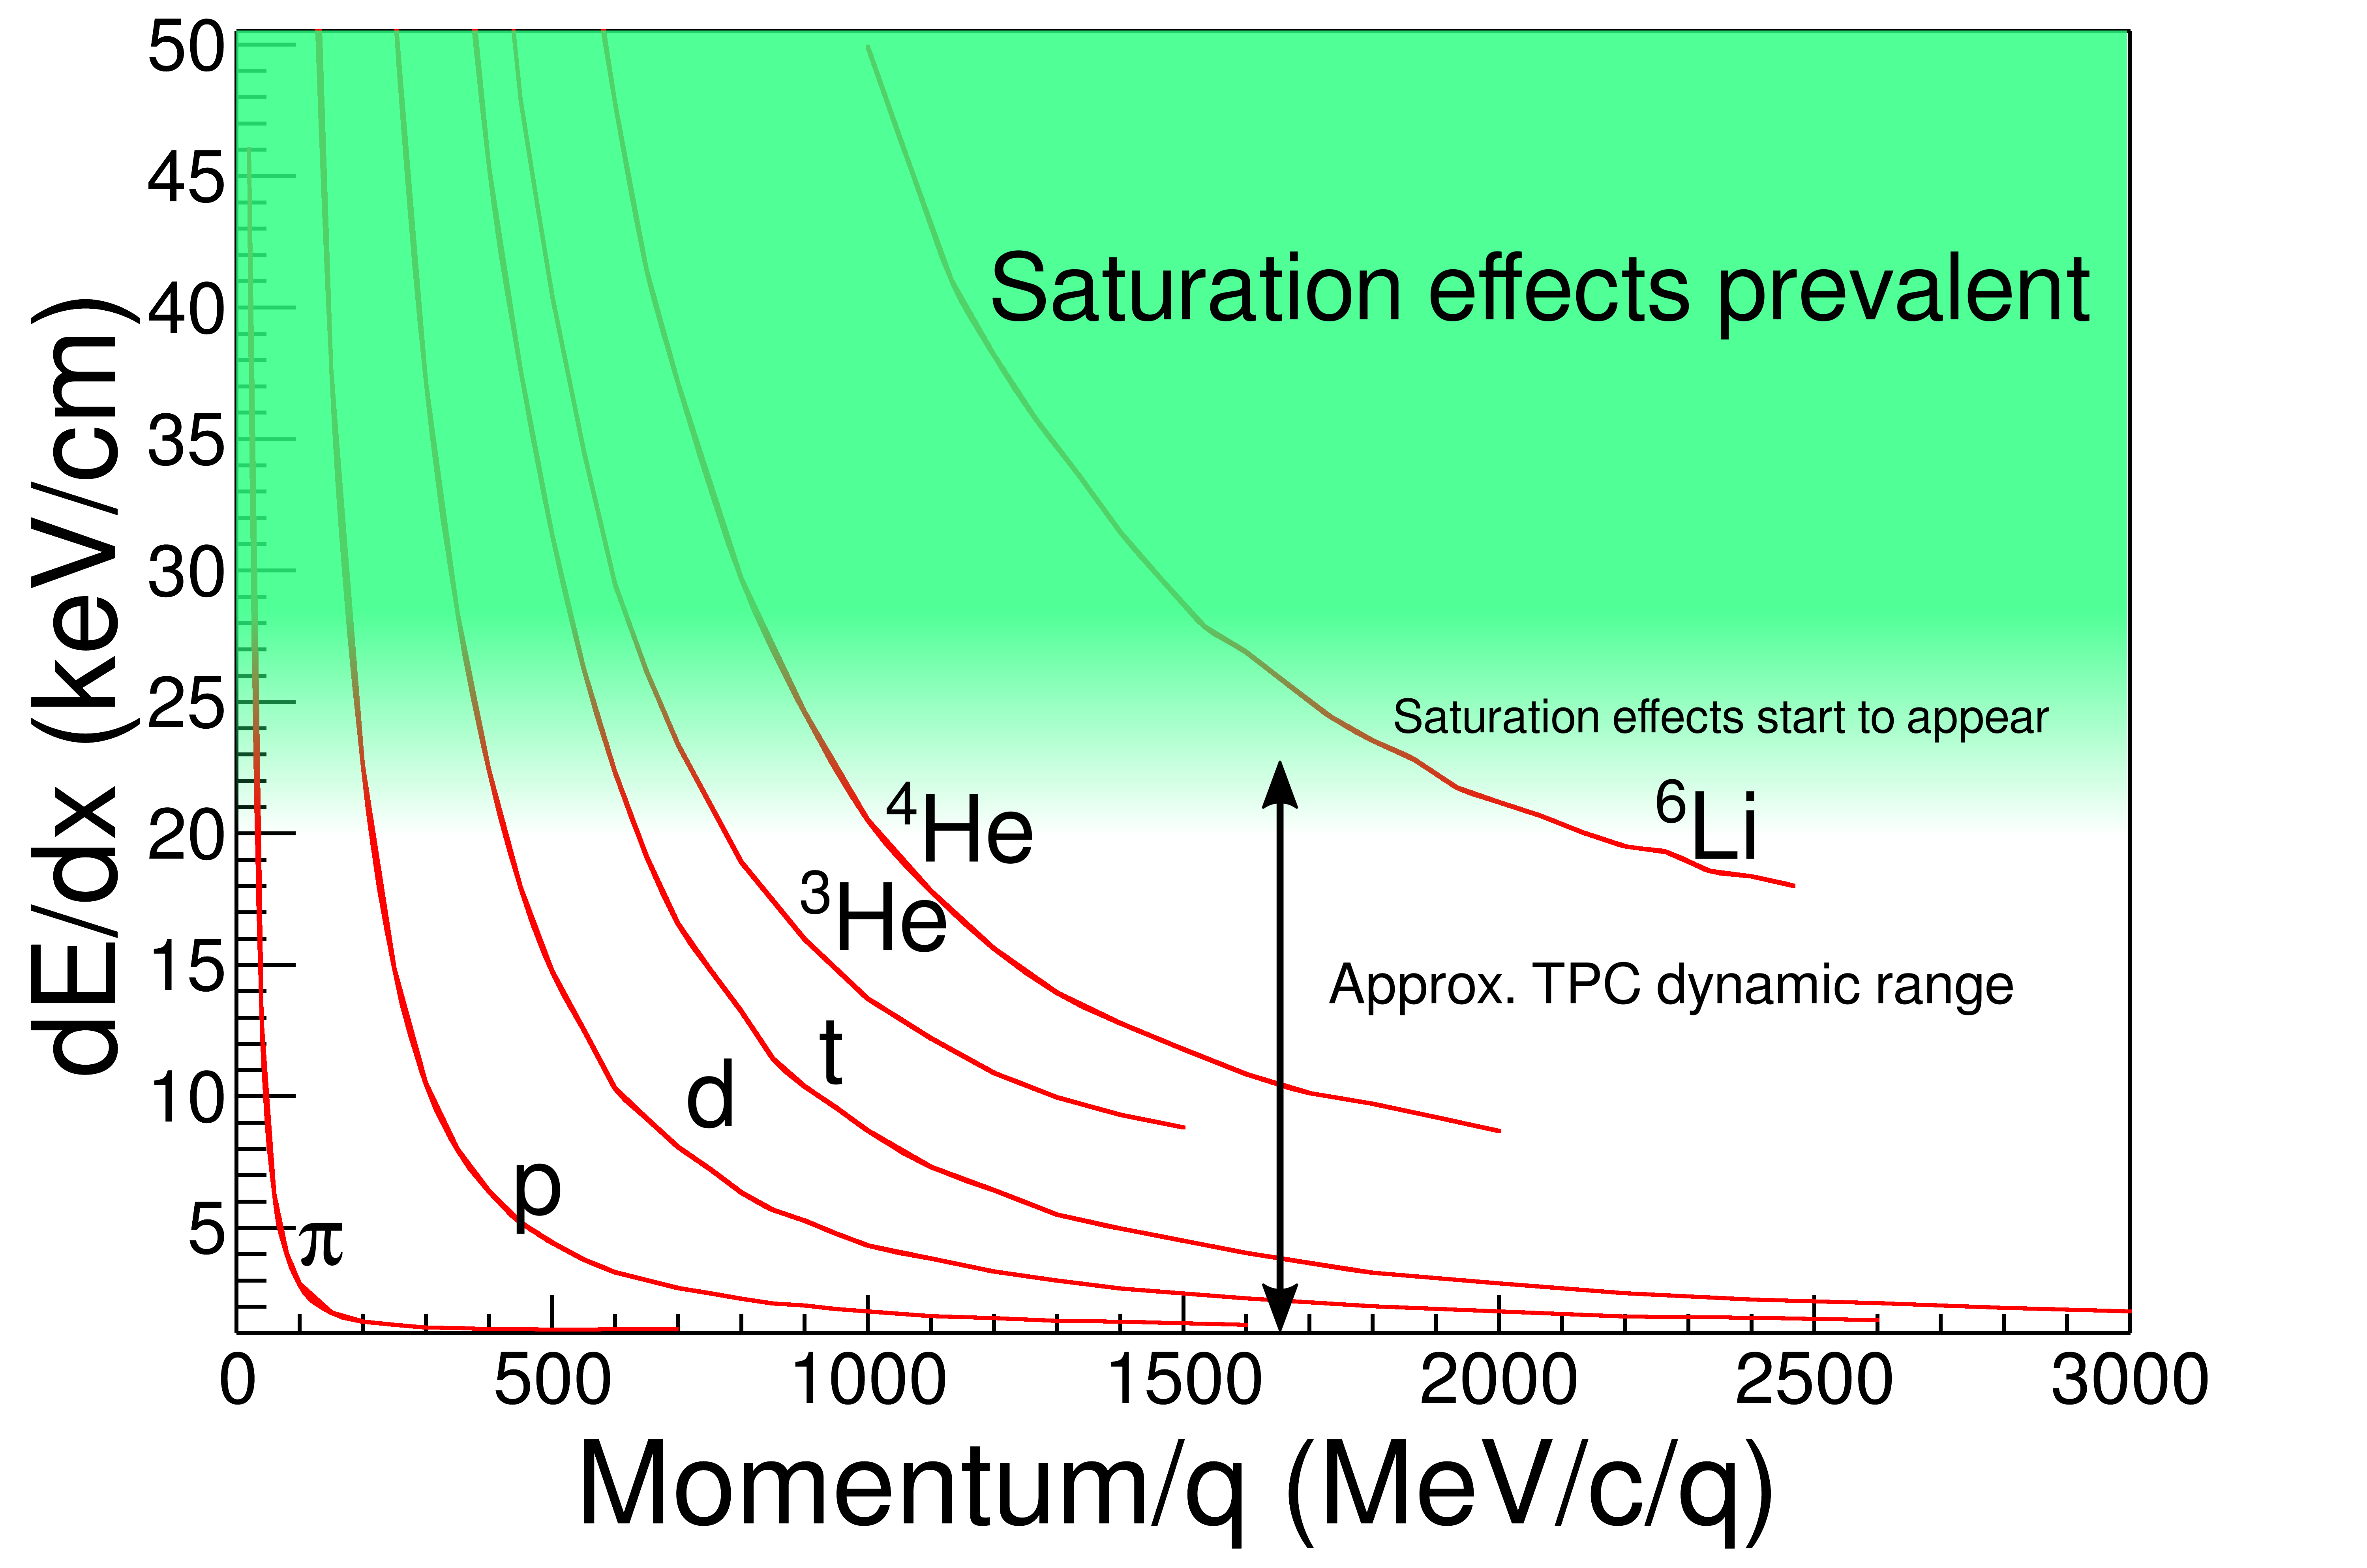
\includegraphics[width=\linewidth]{intrographic}
%\includegraphics[width=\linewidth]{intrographic_2}
\caption{The expected $dE/dx$ lines of different particles are given in red as calculated by Geant4. The approximate dynamic range of the TPC is shown by the vertical bar for the gain setting used in the experiment. Anything outside of this region would be saturated to some degree.}
\label{fig:intro}
\end{figure}

The rapid increase in the stopping powers at low momentum illustrates the degree to which the effective dynamic range can be exceeded and highlights the problems encountered in studies of intermediate HICs, in which light particles with low momenta are abundantly produced along with highly charged particles. Similar problems are encountered when TPCs are used as active targets in direct reaction studies with rare isotope beams \cite{pattpc}. 

Several techniques have been employed to increase the observable range of energy losses. This can be done by lowering the electronics gain of selected readout channels, or by changing the gas amplification at the readout plane in certain areas of the TPC. In the EOS TPC \cite{eos} this was done by decreasing the voltages in select anode wires in the multi-wire readout. With the prototype Active Target TPC lowering or increasing the gain was achieved by decreasing or increasing the electric fields on selected pads within a Micromegas \cite{pattpc}. The results of changing the gas-gain, or the electronics gain, are rather similar in that reducing the gain to sample a range of higher energy loss makes the TPC effectively blind to minimum ionizing particles in  the regions of lower gain.



%DOUBLY DEFINED? IS THIS SUPPOSED TO BE HERE
%\begin{figure}[ht!]
%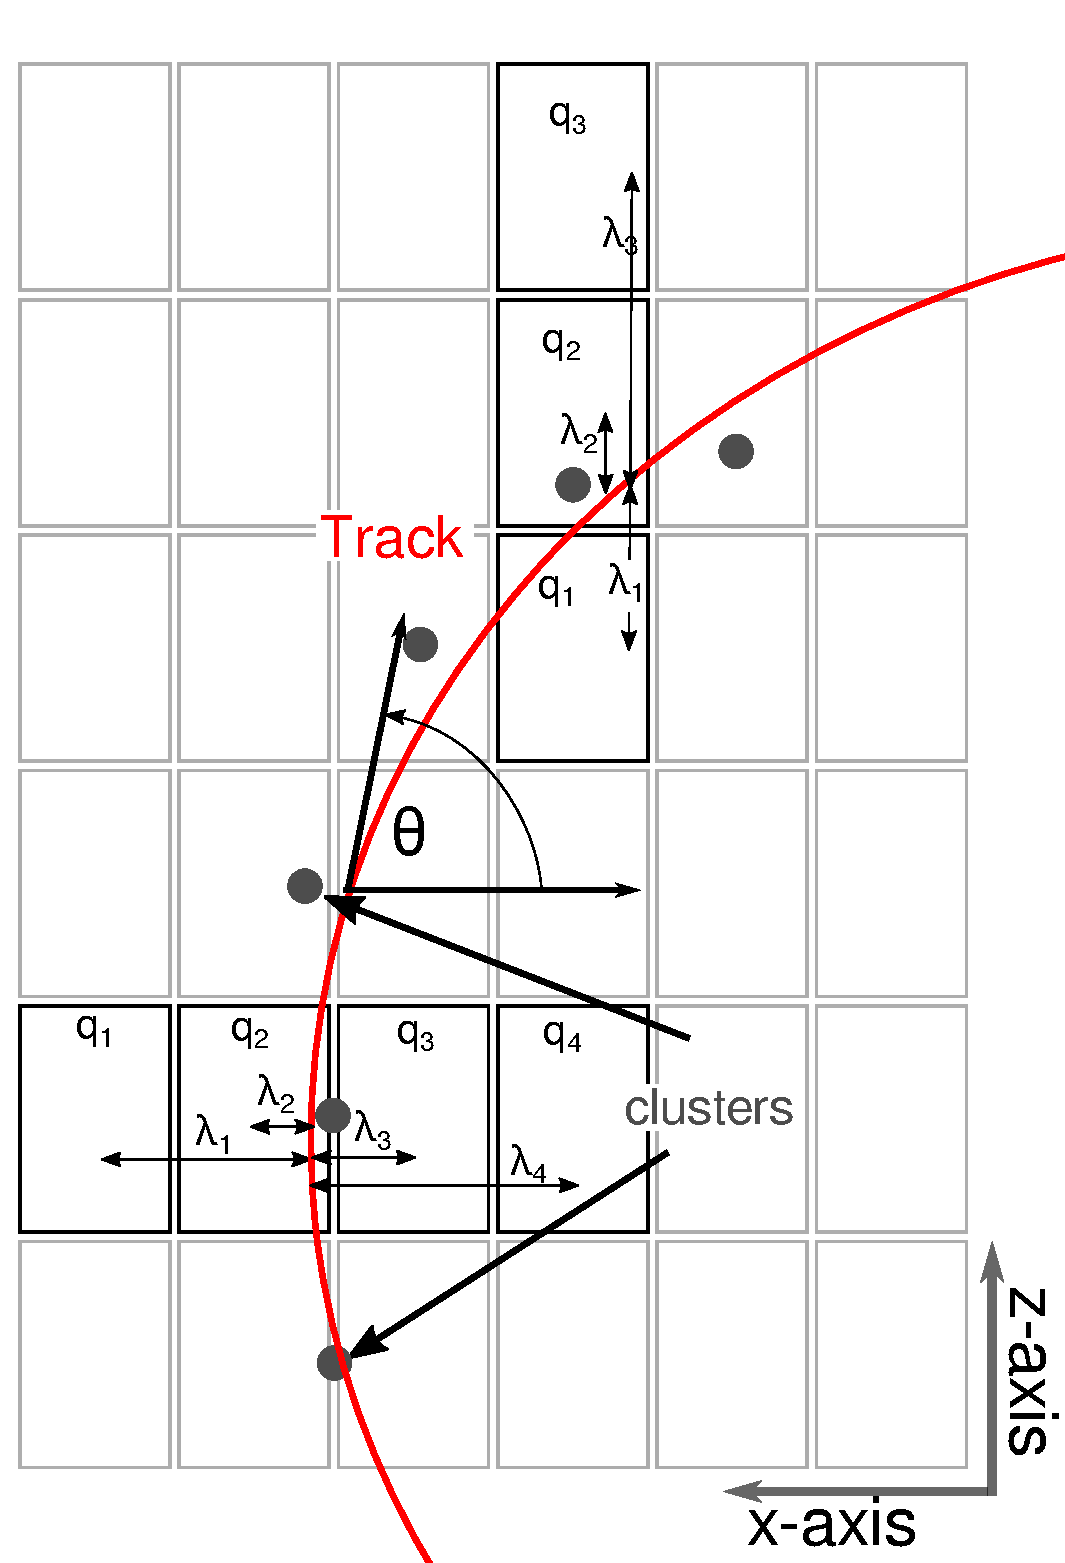
\includegraphics[scale=.5]{top_view_helix_ext.pdf}
%\caption{Cartoon of a top down view of a fit to a track passing through several pads. The bolded pads and the charges $q_i$ represent the hits belonging to that pad and the clusters of the track representing the average position of the track. The three clusters at the bottom are clustered in the $x$-direction for the upper three are clustered in the $z$-direction. The estimated position of the avalanche is given by the track fit, and the position from the center to each pad to the $\bar{x}$ position is given as $\lambda_i$.}
%\label{fig:topview}
%\end{figure}

We define the clustering direction depending on the angle of the track, at the point of each cluster, with respects to the $x$ axis, defined as $\theta$. For example, the crossing angle is defined as $90^{\circ}$ for a track going along the $z$ axis, and $0^{\circ}$ for a track going along the $x$ axis. In the case that the crossing angle is $45^{\circ} < \theta \leq 90^{\circ} $ the clustering direction is along the $x$ axis. For $0^{\circ} < \theta \leq 45^{\circ}$ it is along the $z$ axis. 

 The position along the clustering direction is calculated by weighting the individual hit's positions by their charges $q_i$ and getting the mean value. The other direction is set to the center of the pad. For example, if we are clustering along the $x$ axis for a cluster, the $z$-position is set to the center of the pad in the $z$-direction and vice versa. 
 


\subsection{Method of Desaturation}
We will use the term ``desaturation'' for our process of correcting the charge values of the saturated pads. Figure \ref{fig:satpad} shows a typical situation of saturated signals. When an avalanche causes a large induced signal, the pads directly underneath collect the largest charge becoming saturated, denoted as $q_{2'}$ and $q_{3'}$. Pads further away experience smaller, non saturating charges, denoted as $q_{1}$ and $q_{4}$. Though we do not know the saturated charge values, the distribution of all charges must follow the PRF which we have experimentally measured. From the clusters crossing angle, we can get the corresponding parameters for the PRF as described above and in Fig.~\ref{fig:normsigma}.

We assume the distance of each pad to the track, $\lambda_i$, is fixed, defining the fraction of charge each pad receives as given by the $PRF(\lambda_i)$ function. 


\begin{equation}\label{eq:chi}
\chi^2 = \sum_i \frac{(q_i^{\mathrm{obs}} - q_i^{\mathrm{expect}})^2}{q_i^{\mathrm{expect}}}
\end{equation}

To determine the best estimate for the charge values of each saturated pad, a chi squared function is minimized, given in  Equation \ref{eq:chi}, where $q_i^{\mathrm{obs}}$ are the observed, non-saturated charges $q_{1}$ and $q_{4}$, and $q_i^{\mathrm{expect}}$ are the charges we expect to observe, calculated as $q_i^{\mathrm{expected}} = Q\cdot PRF(\lambda_i)$. The charges $q_{2'}$ and $q_{3'}$, make up the unknown variable and are allowed to vary in the $\chi^2$ minimization, where they are added to make up the total expected charge $Q$.


\begin{figure}[ht!]
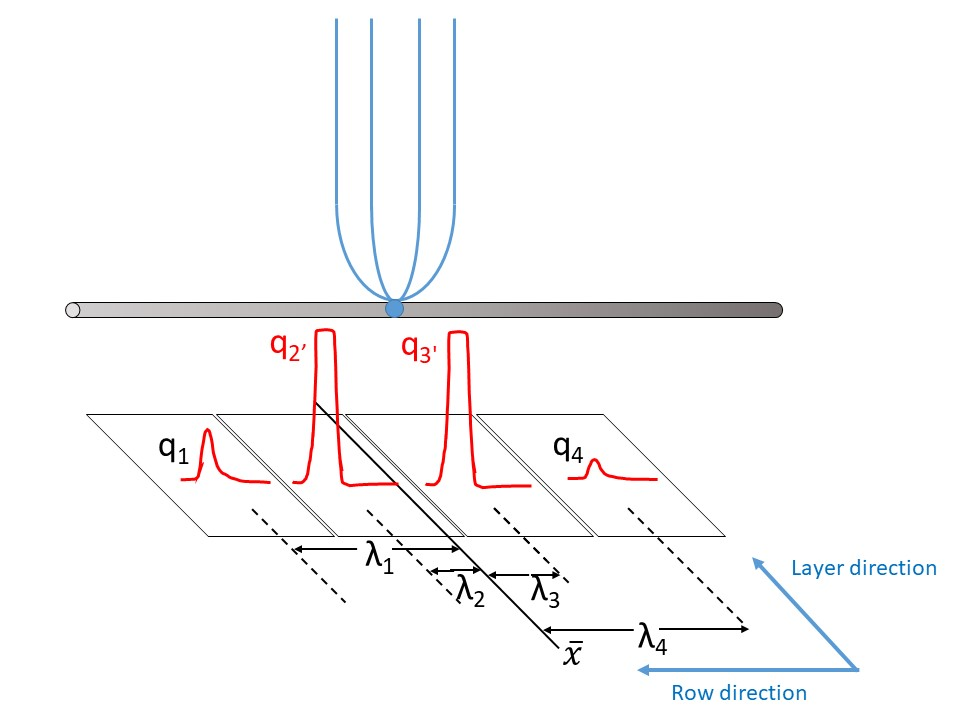
\includegraphics[width=\linewidth]{saturated_pads}
\caption{A typical case of a saturating event. The red pulses represent the time bucket signal for each collected charge. The pads directly underneath the avalanche point, $q_{2'}$ and $q_{3'}$, are saturated while pads farther away, $q_1$ and $q_4$ are not saturated.}
\label{fig:satpad}
\end{figure}

Shown in Fig.~\ref{fig:cocktail} is a typical cocktail event, where one particle enters the TPC volume at a time and parallel to the pad plane, representing an ideal case for momentum and $dE/dx$ determination; as it does not suffer from inefficiencies of high multiplicity events seen in the collision experimental data.  

\begin{figure}[ht!]
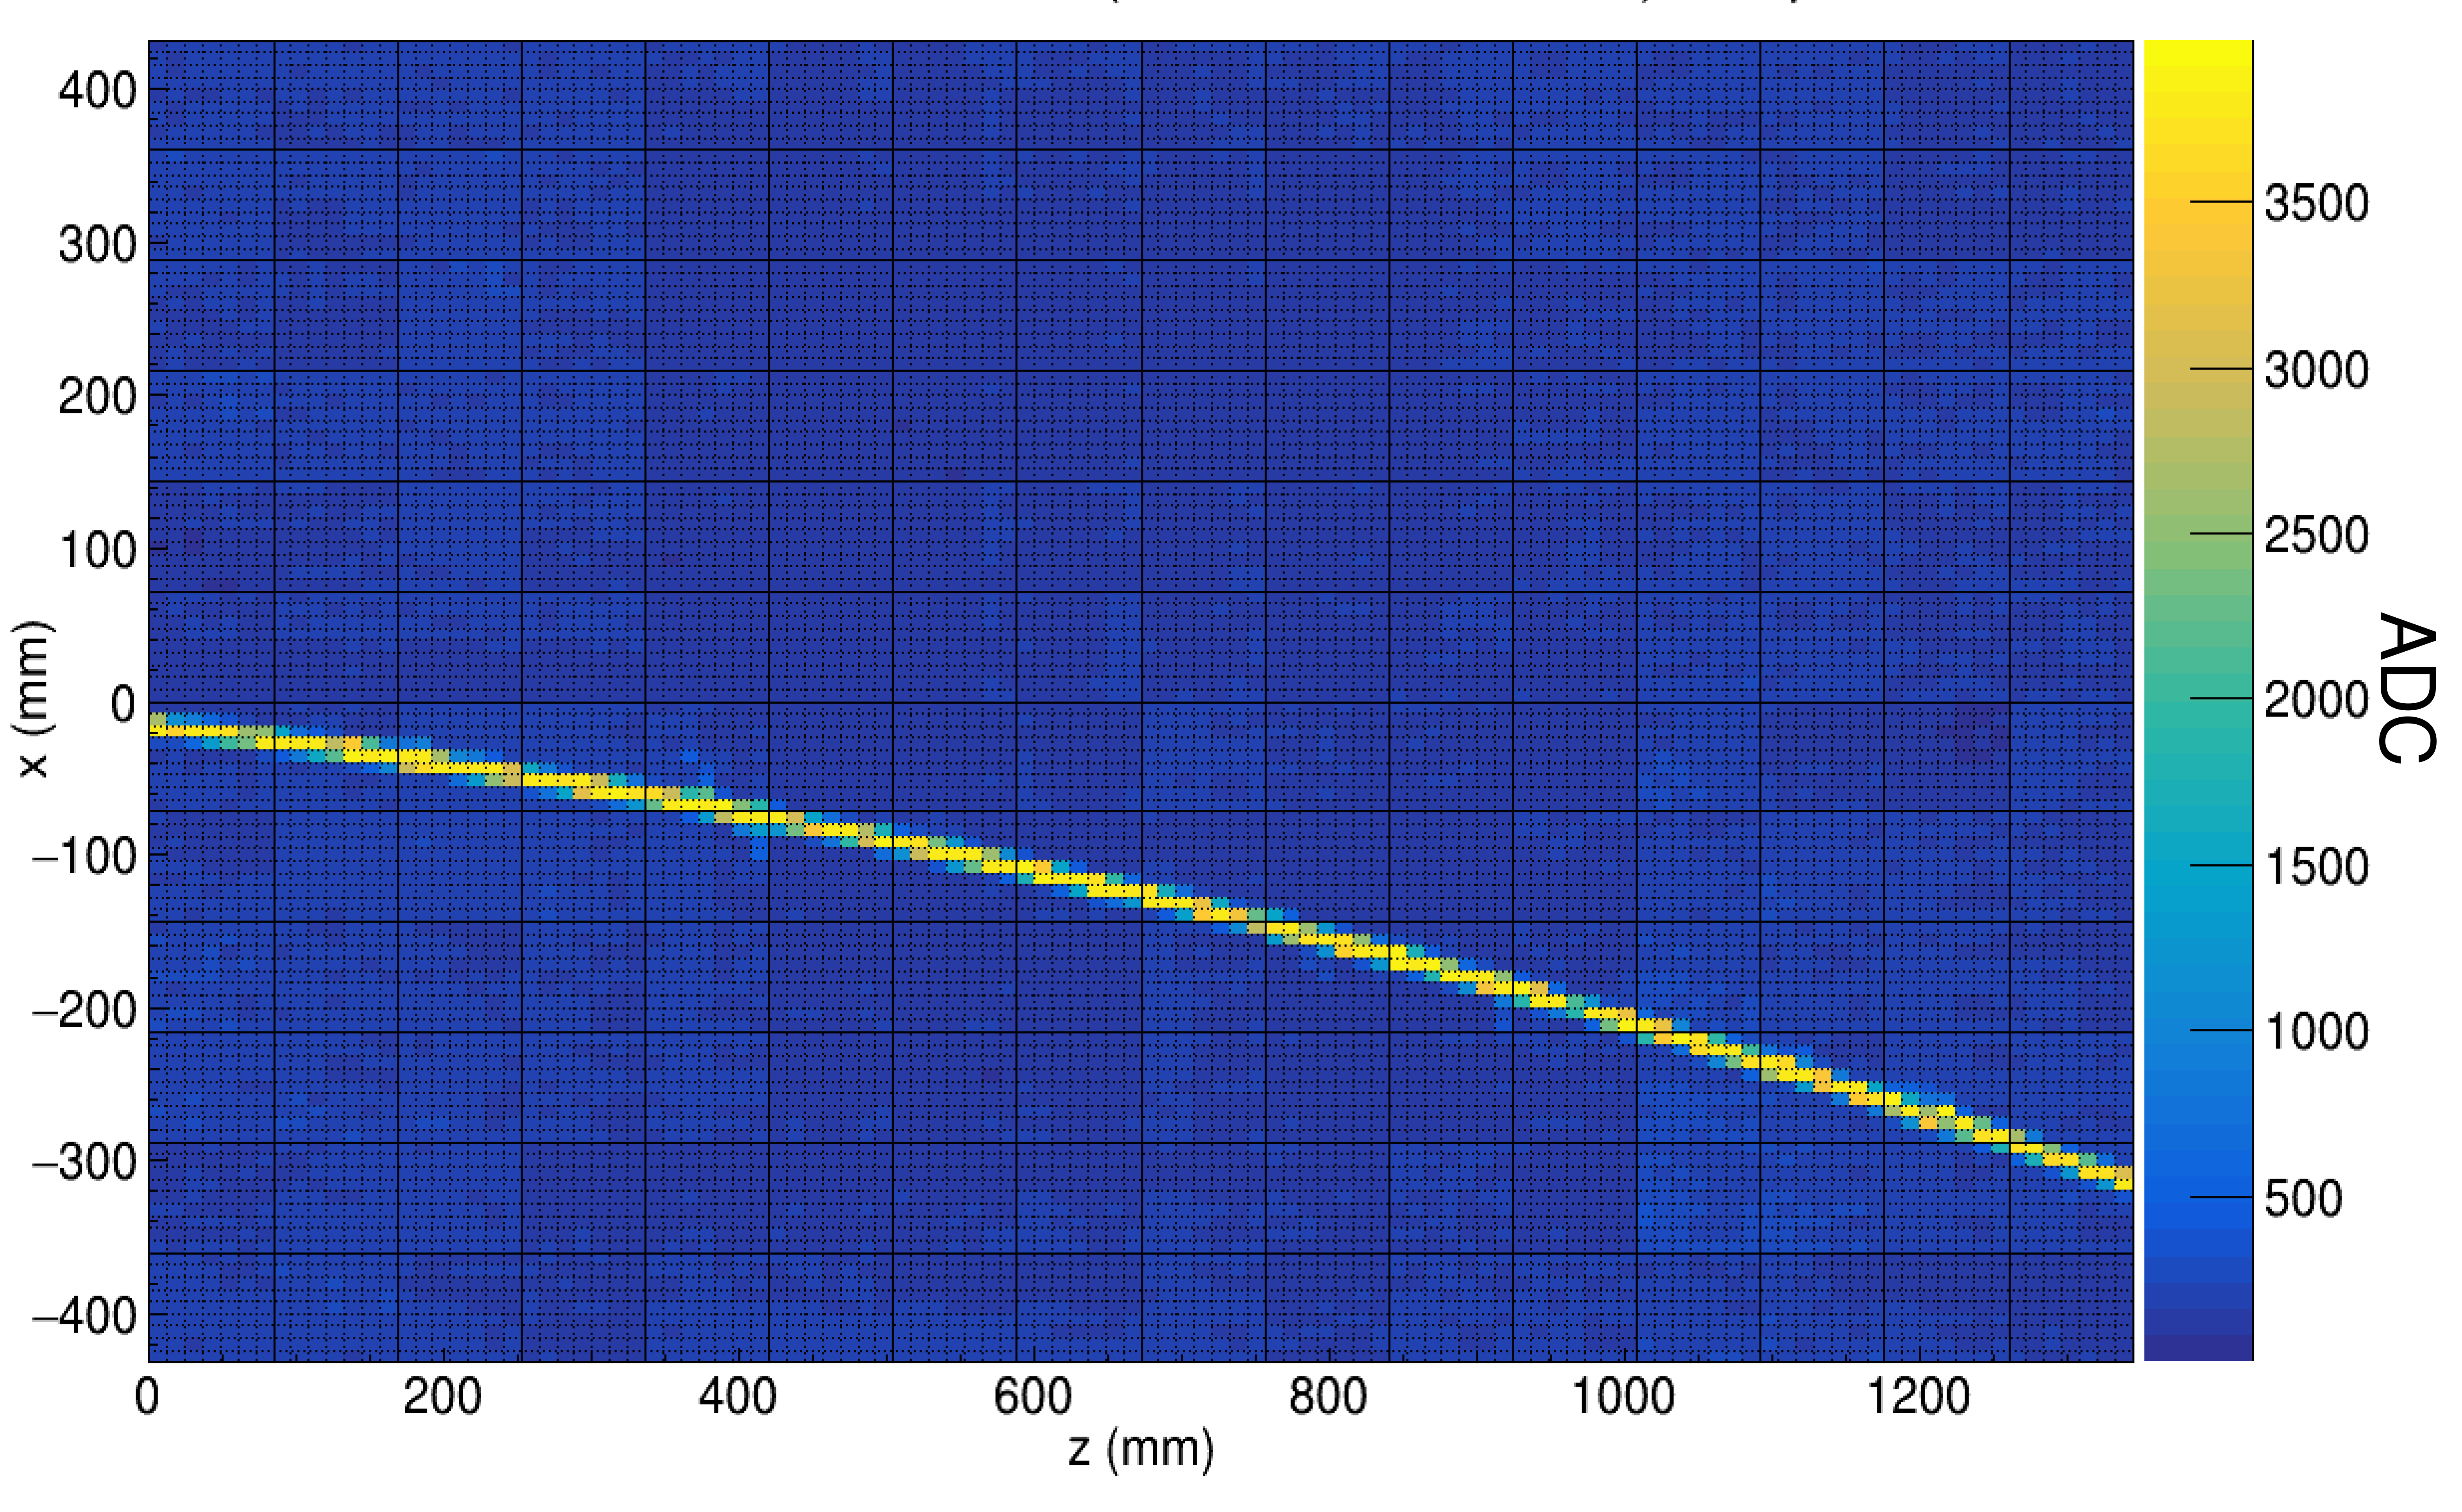
\includegraphics[width=\linewidth]{cocktail.png}
\caption{Pad plane projection for a cocktail event in the TPC.}
\label{fig:cocktail}
\end{figure}

\begin{figure}[ht!]
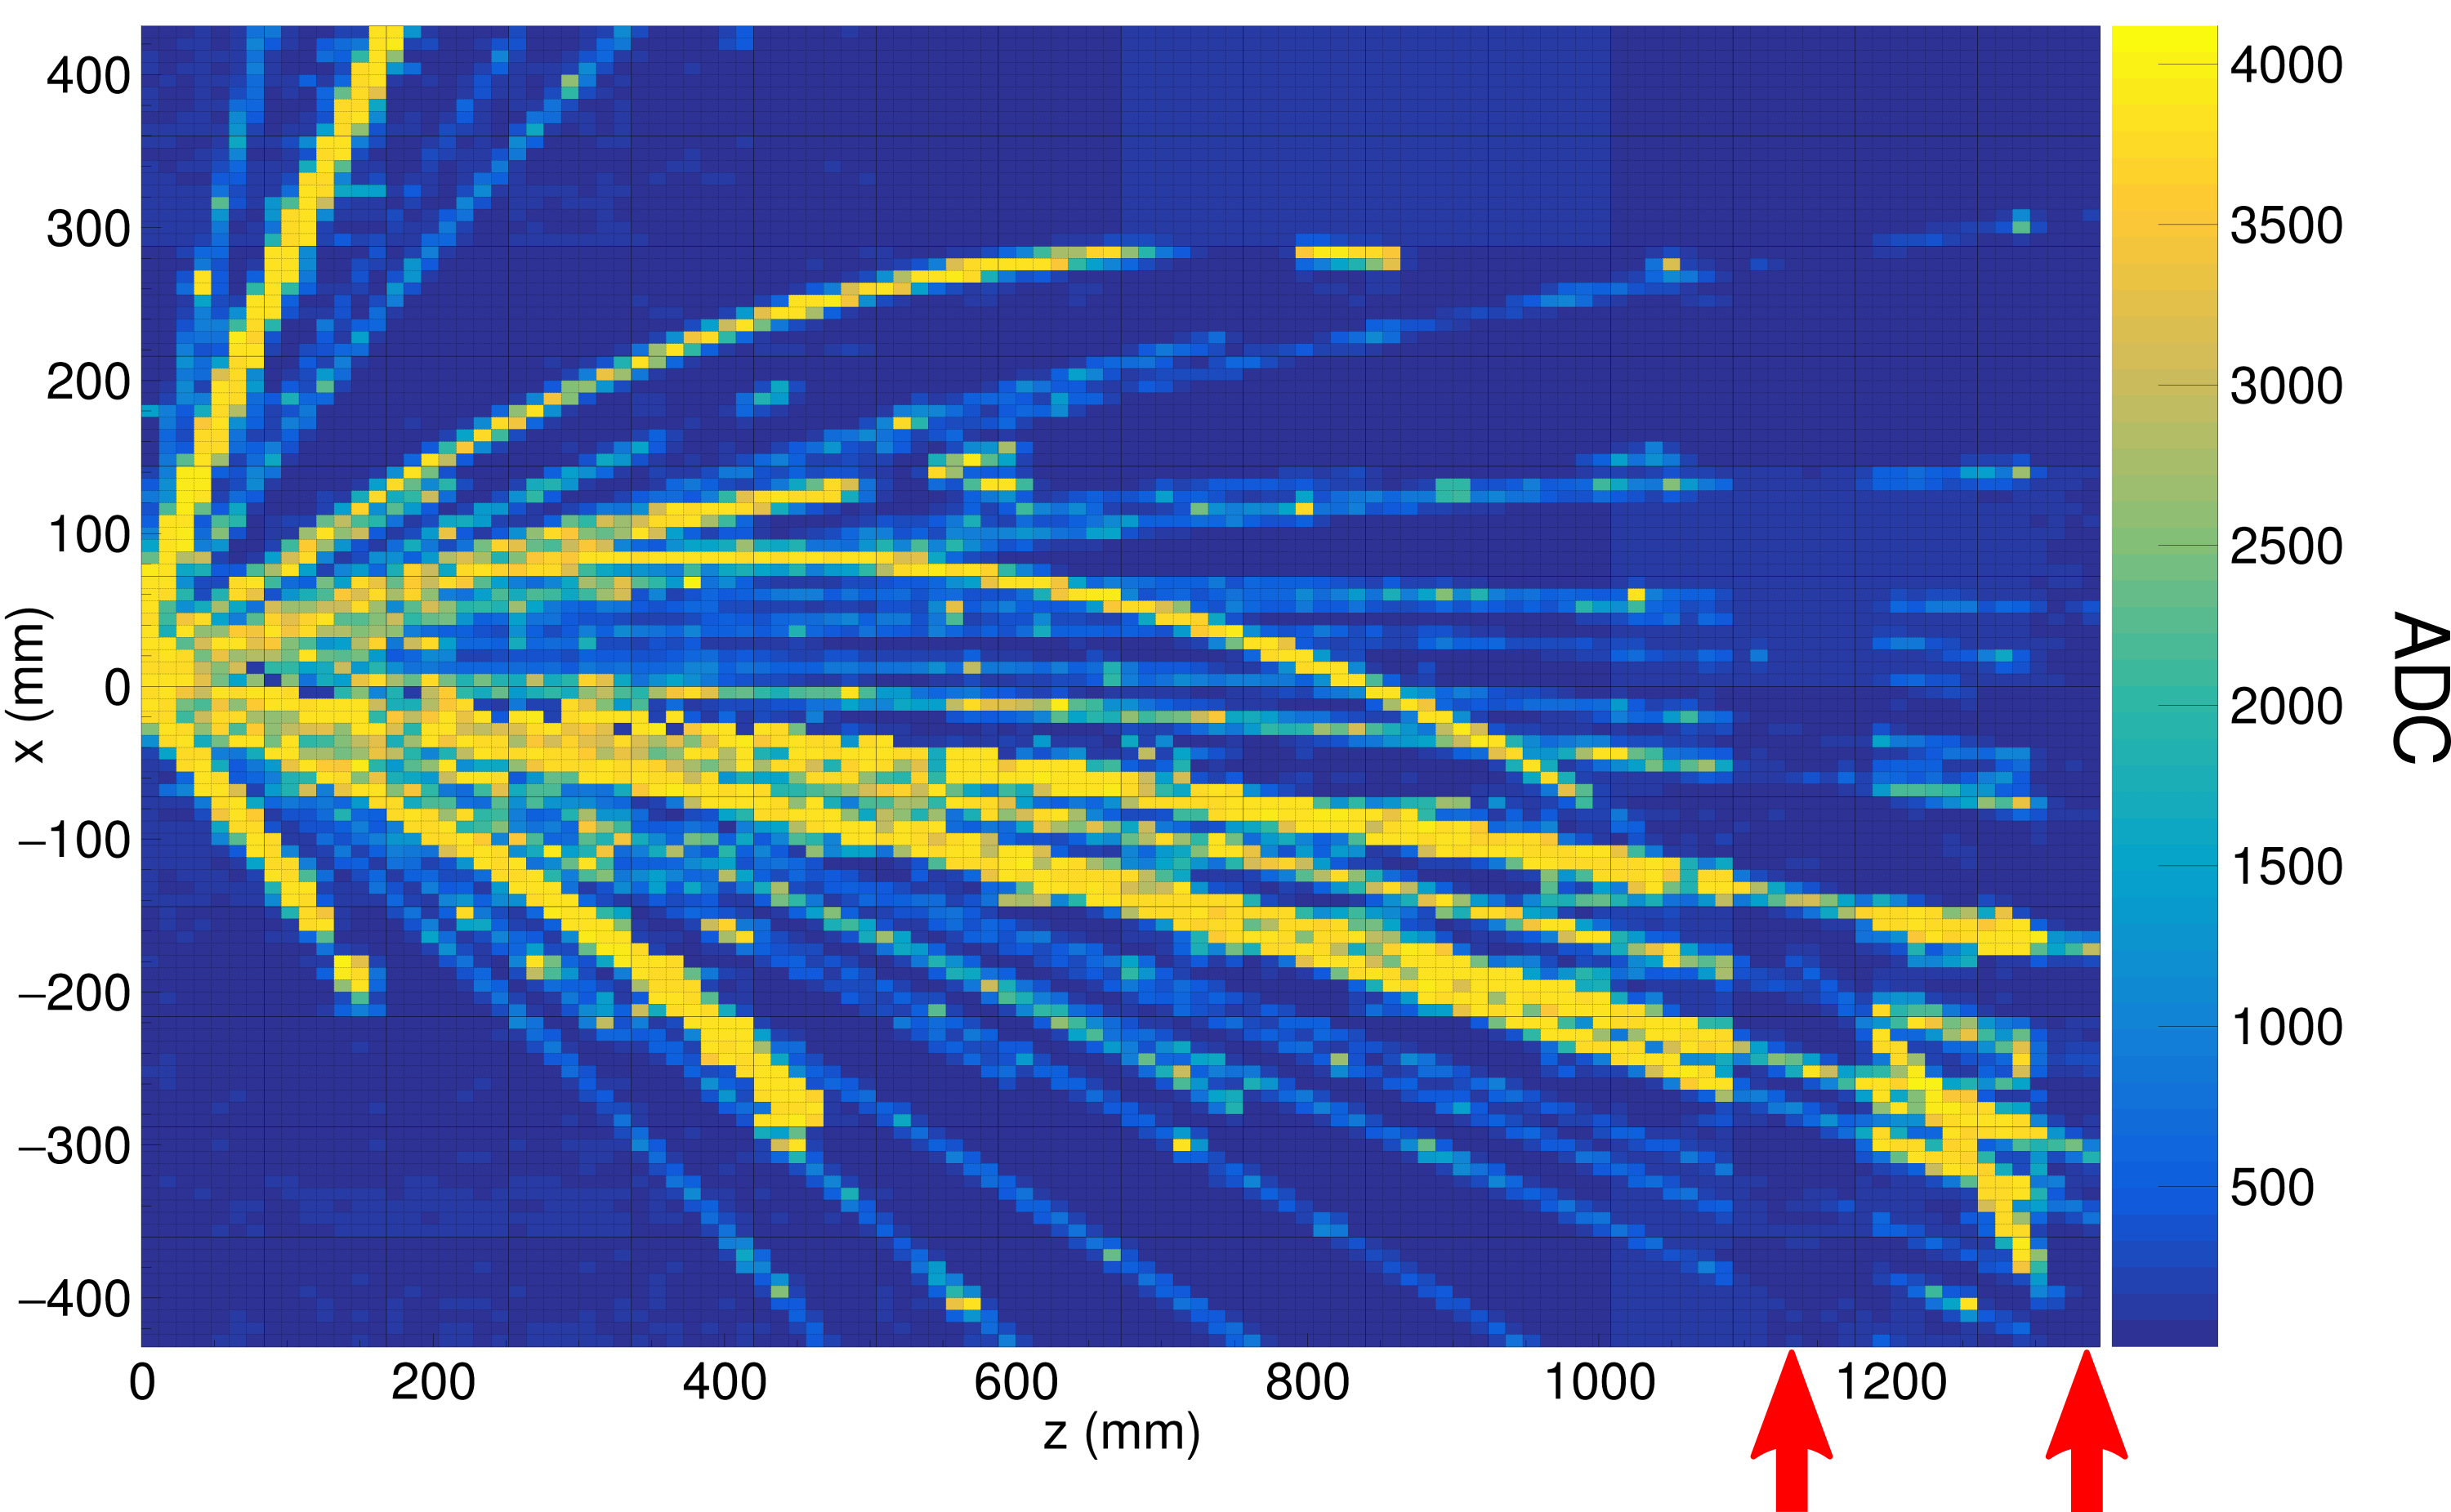
\includegraphics[width=\linewidth]{data.png}
\caption{Pad plane projection for a collision event in the TPC. Highlighted by red arrows are two regions of anode wires which had a reduced voltage of 1214 V. The voltage of the rest of the TPC anode wires are 1460 V. The reduction in voltage reduces the gain by a factor of about 10. }
\label{fig:data}
\end{figure}


\begin{figure*}[t]
\centering
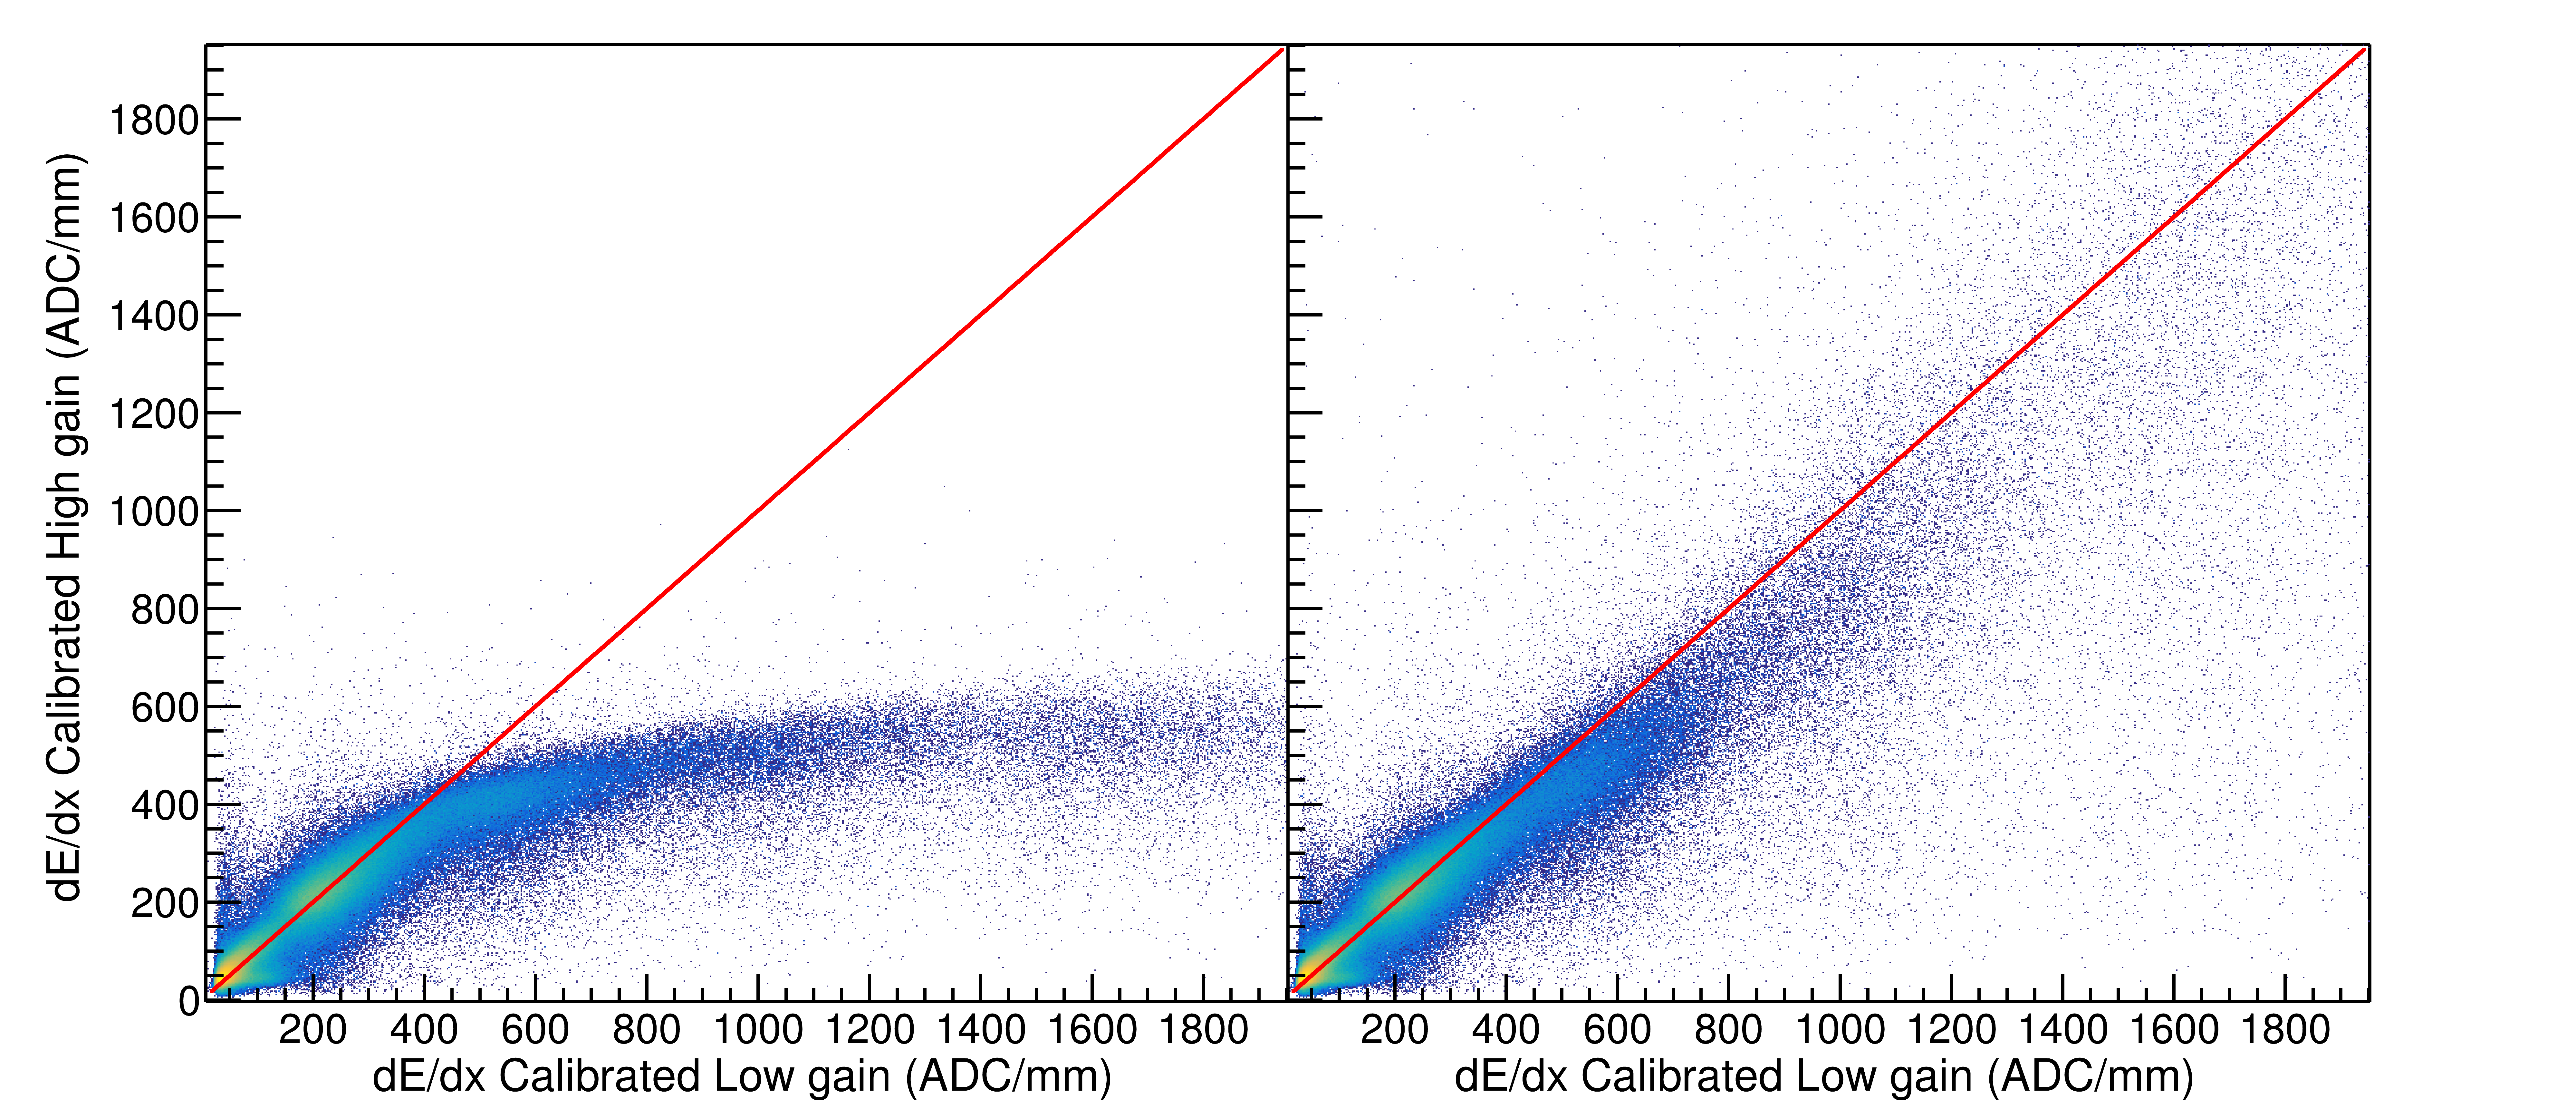
\includegraphics[width=\linewidth]{dedx_compare}
\caption{The left panel shows the high gain stopping power vs low gain when the method of desaturation was not applied. In the right panel the desaturation technique was applied to the high gain region. The low gain does not suffer from saturation and represents the true $dE/dx$ value.}
\label{fig:lowvshigh}
\end{figure*}

\begin{figure*}[t]
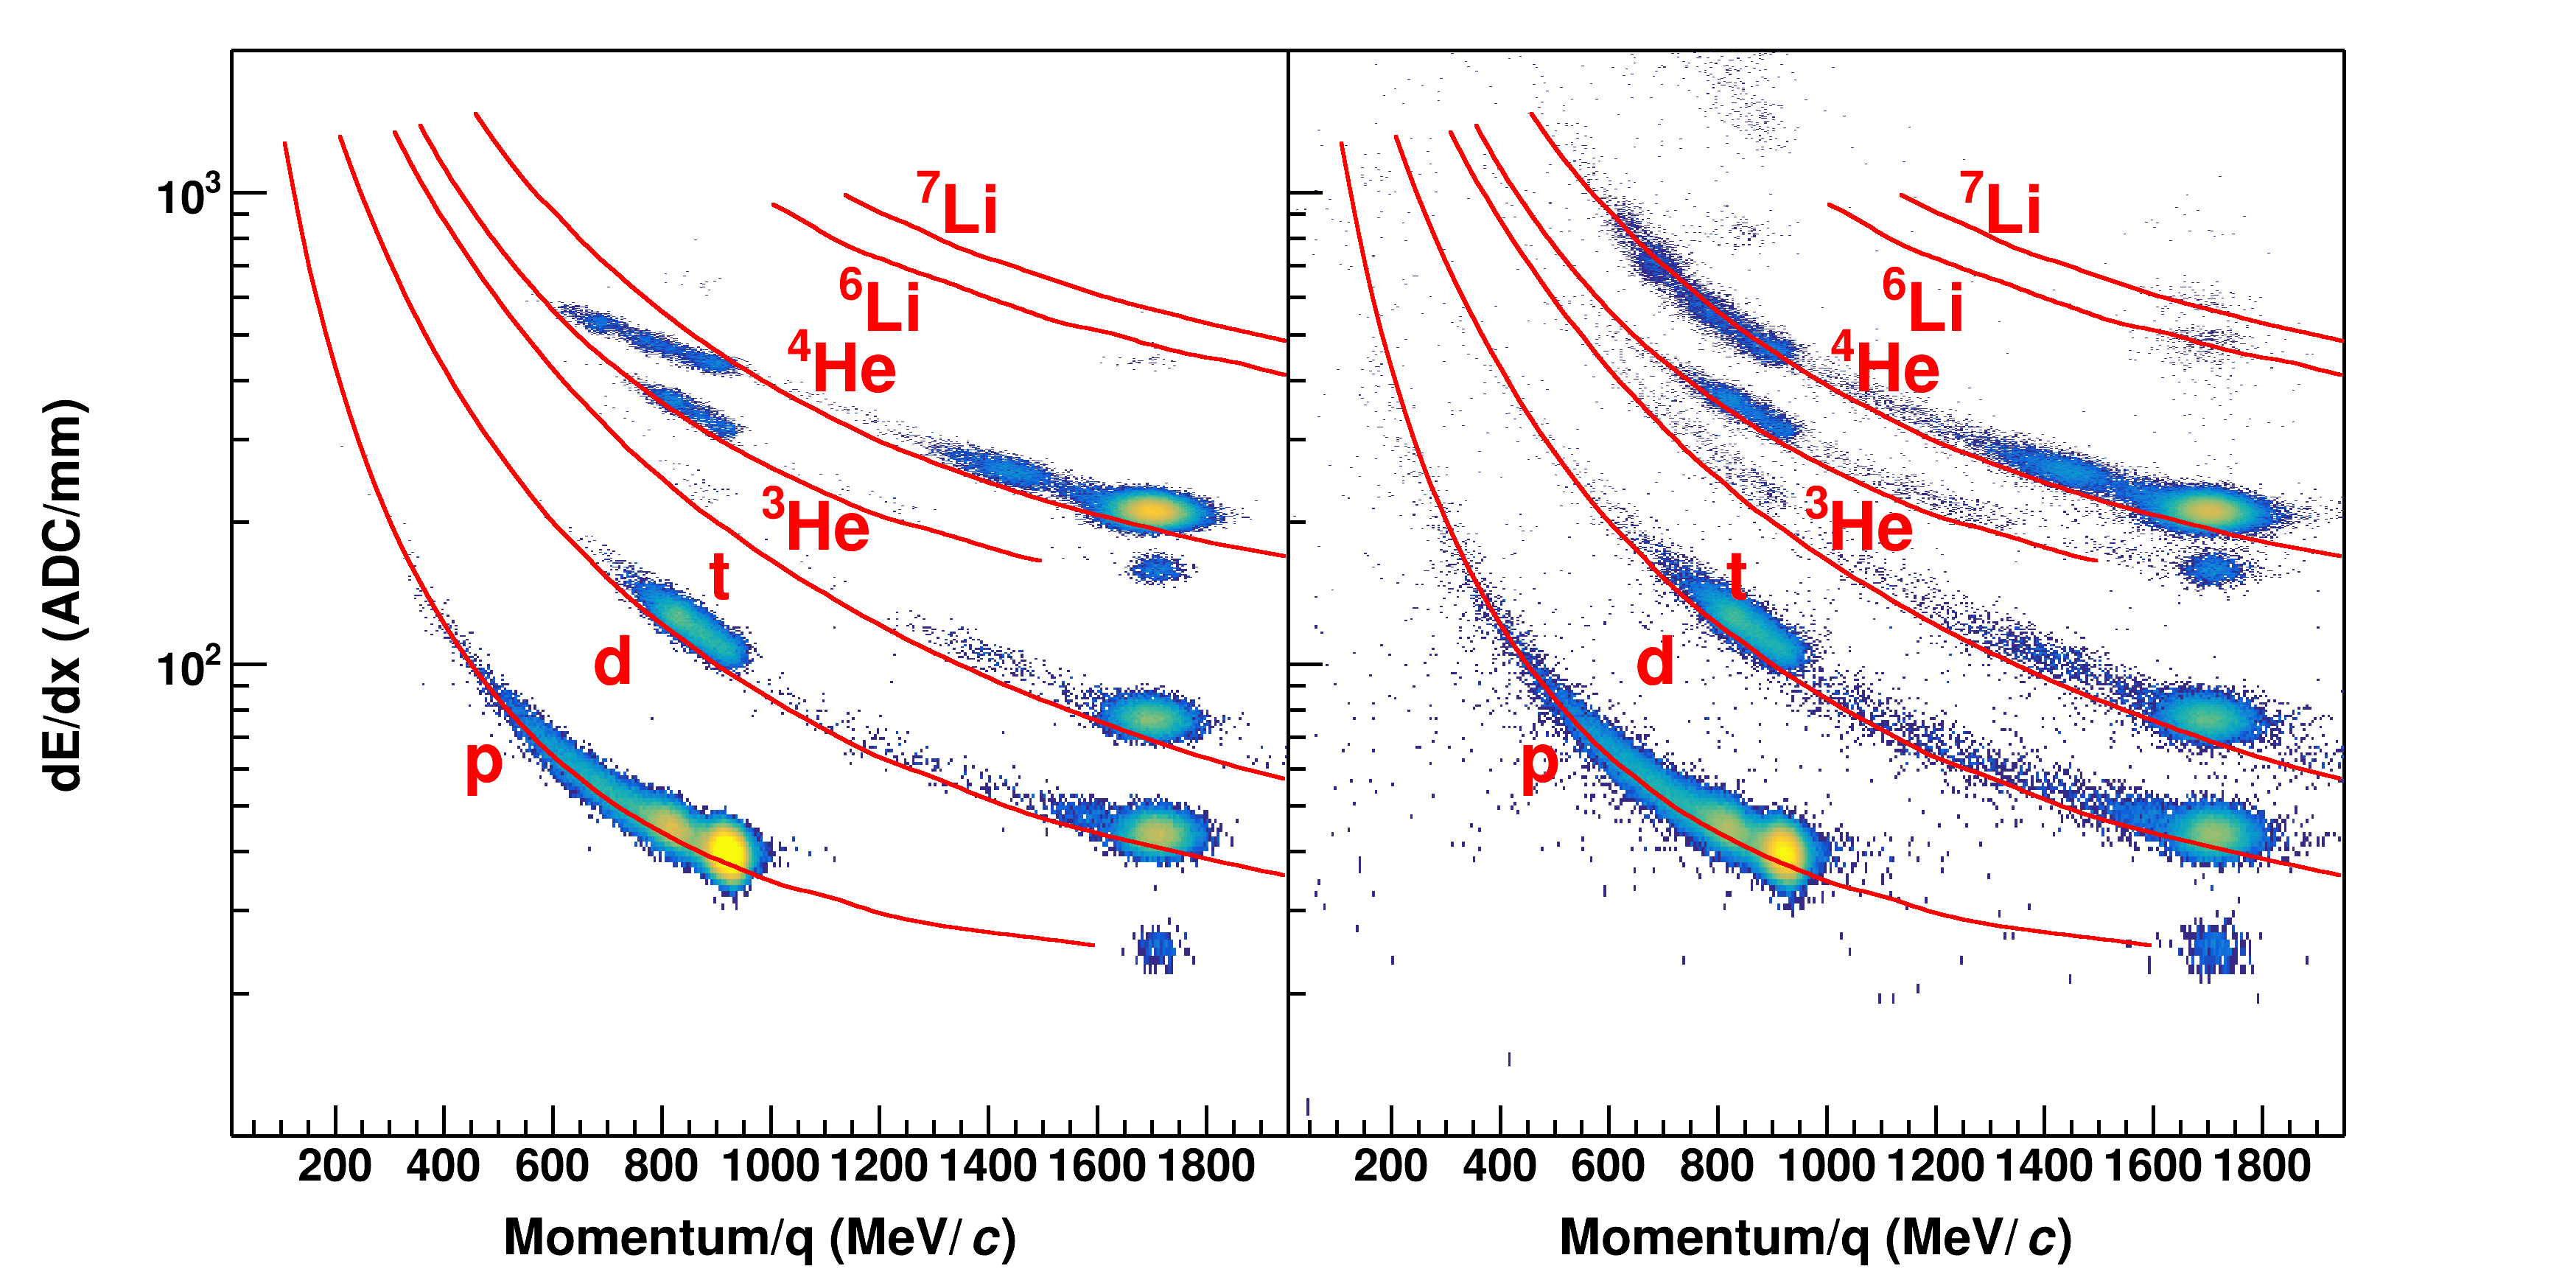
\includegraphics[width=\linewidth]{cocktail_combine.png}
\caption{Uncorrected (left panel) and desaturated (right panel) cocktail data.}
\label{fig:cocktail_combine}
\end{figure*}

\begin{figure*}[t]
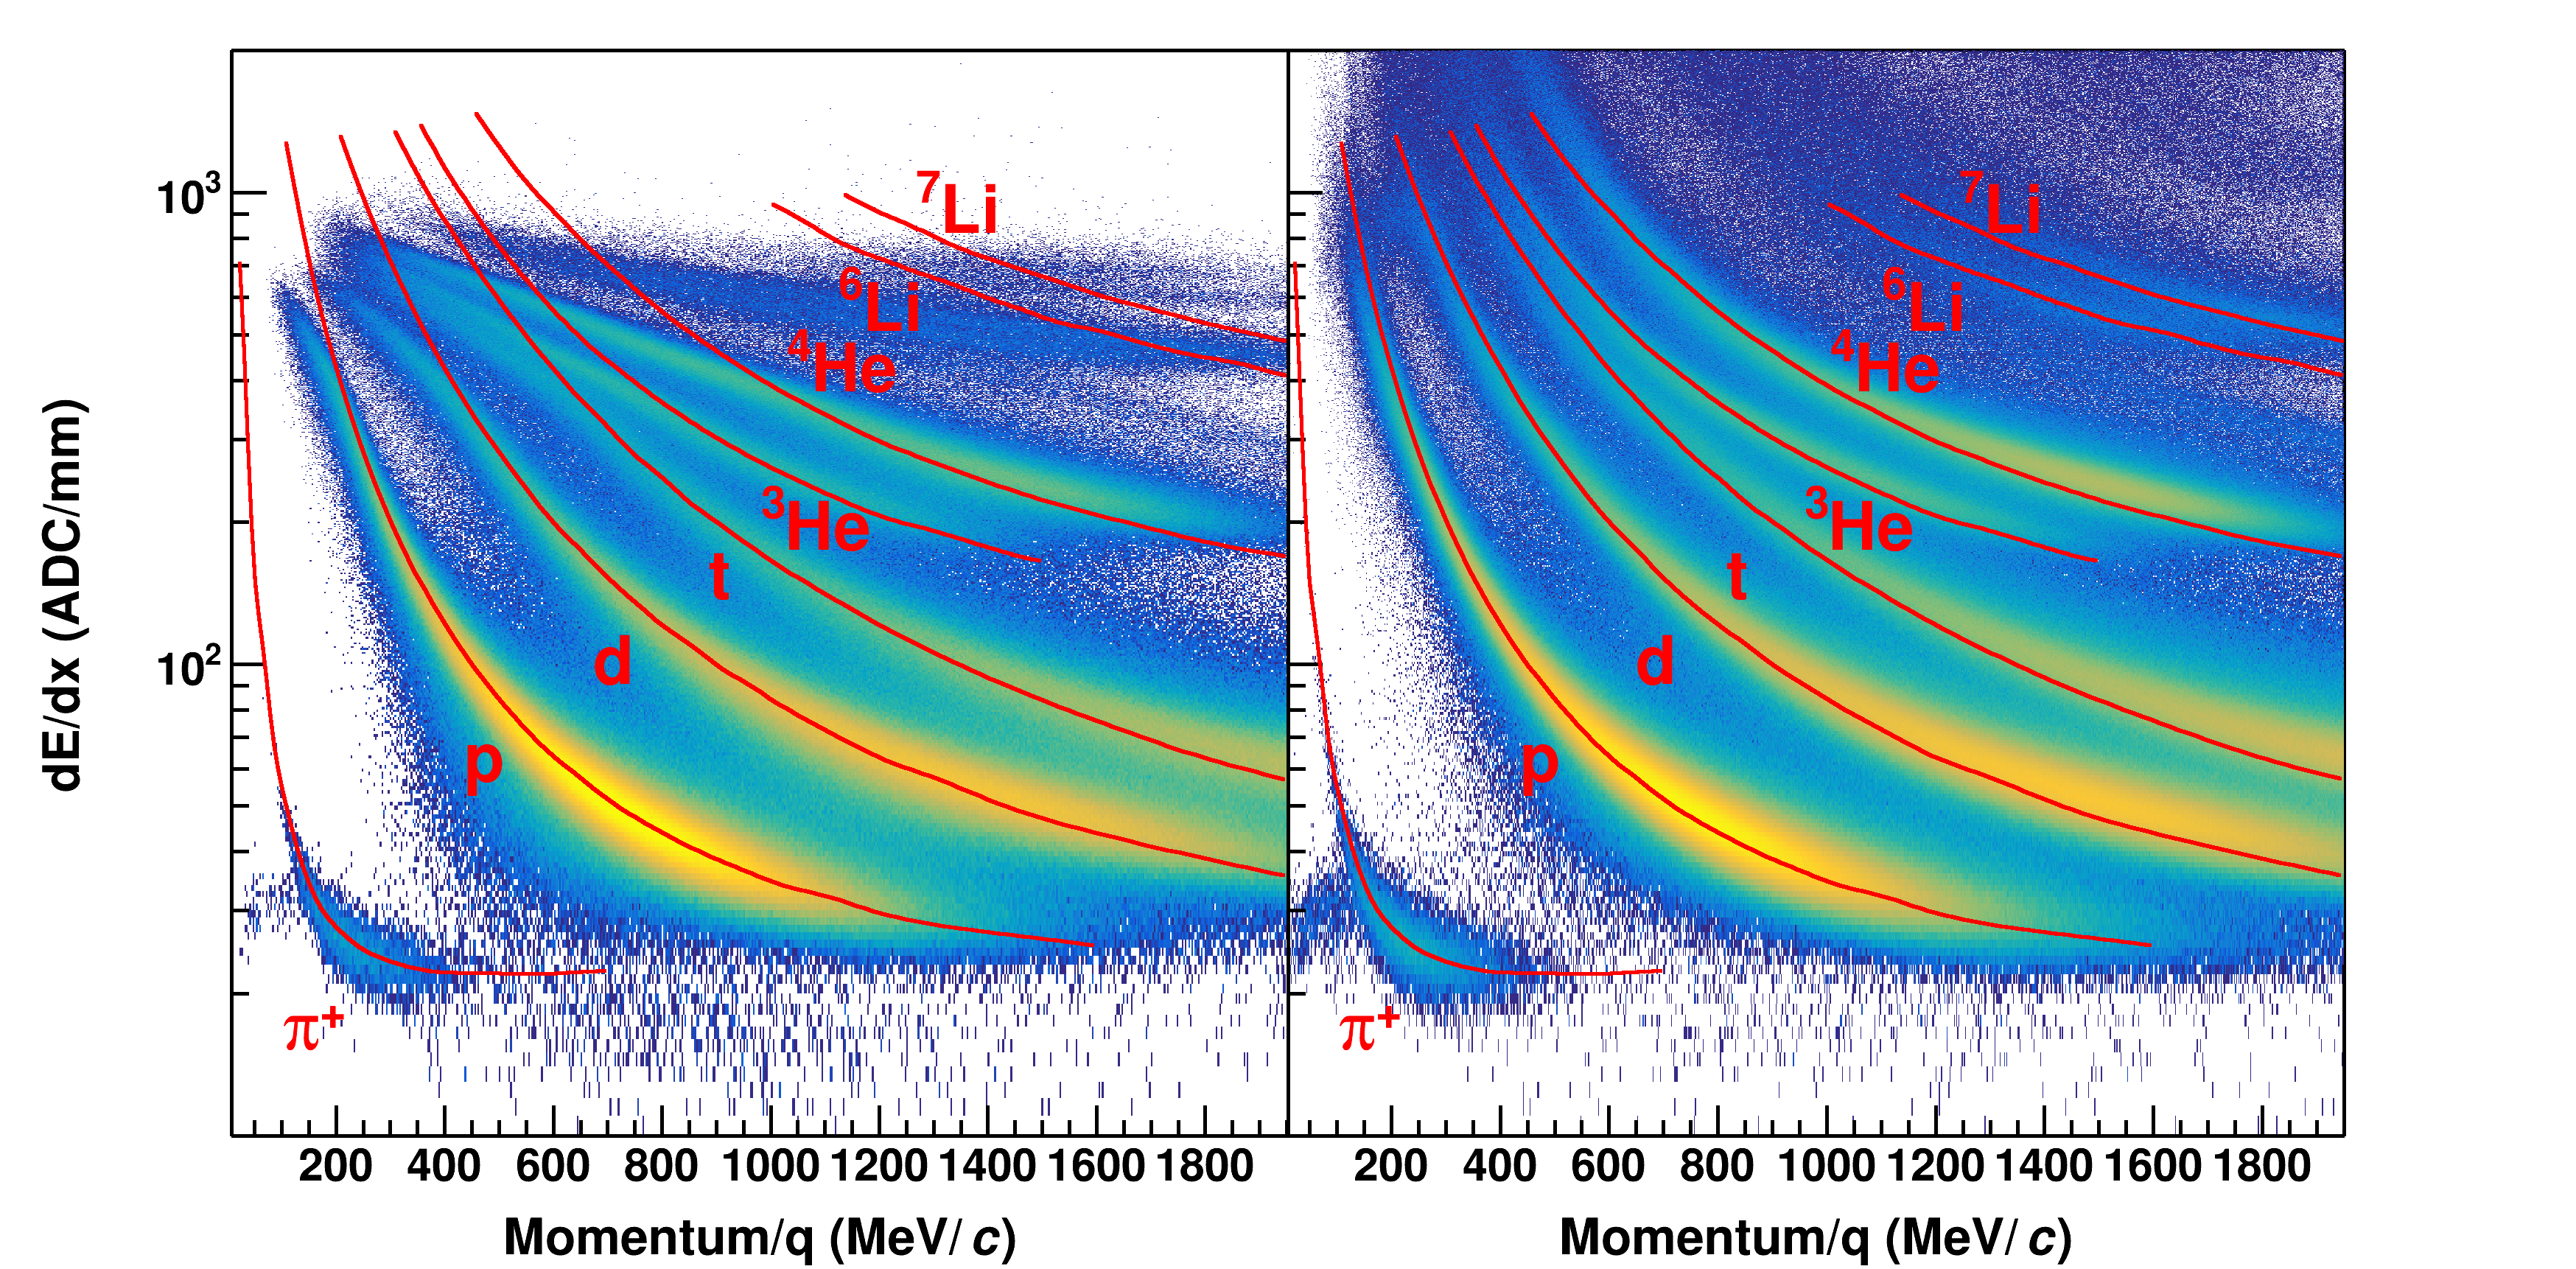
\includegraphics[width=\linewidth]{data_combine}
\caption{Uncorrected (left panel) and desaturated (right panel) collision data at polar angles of $\theta < 40^{\circ}$ and azimuthal angles between $-80^{\circ} < \phi < 80^{\circ}$}
\label{fig:data_combine}
\end{figure*}

Tracks which saturate pads in the high gain region are not saturated in the low gain region. By comparing the dE/dx values of these two sections, we can directly measure the success of the desaturation in the high gain regions using the method described above.  
 
In Fig.~\ref{fig:lowvshigh}, the effect of saturation can be seen in the high gain region for the uncorrected data. For signals below 400 ADC/mm \footnote{Un-calibrated ADC channels in arbitrary units.} the electronics are not saturated, and therefore the high and low gain sections agree. The data starts to saturate above 400 ADC/mm in the high gain channels eventually reaching a plateau while the low gain sections are not saturated and provide the true $dE/dx$ values.
 After applying the desaturation method, the correlation between the high and low gain sections is restored, as seen in Fig.~\ref{fig:lowvshigh}. From this comparison, we infer that the correction works up to signals of 2000 ADC/mm, increasing the dynamic range by a factor of at least 5.


Comparing the low to high gain sections directly validates the desaturation technique, but the goal  of this exercise is to improve the particle identification (PID). In the following PID plots the red lines represent the most probable energy loss as given by Geant4 straggling functions. A linear calibration was performed to convert keV in Geant4 to ADC in the experiment given by $ADC/mm = 19\;keV/cm$.

There are pronounced PID lines of several particle species in both the uncorrected and corrected cocktail beam PID shown in the subplots of Fig.~\ref{fig:cocktail_combine}. Three ovals around a momentum of 1700~MeV/$c$/q and two near 900~MeV/$c$/q correspond to the three $B\rho$ settings injected into the TPC. The tails of the PID lines are resulting from the particles passing through the walls and other materials outside the main detector volume, therefore lowering the initial momentum. 

The uncorrected data in Fig.~\ref{fig:cocktail_combine} shows the effects of saturation; the PID lines deviate from their theoretical expectations starting at around 400~ADC/mm eventually reaching a plateau. After applying the desaturation technique, we see a large improvement, most notably for the He and Li particles, which suffer the most from saturation. A more subtle improvement of the lighter particles, (p, d, t), can also be seen in the PID lines at lower momenta.

Looking at the collision data, shown in Fig.~\ref{fig:data_combine}, we also see a similar result. In the collision data, the PID suffers from more background and inefficiencies than the cocktail beam, nevertheless we can see a similar improvement in the PID lines when comparing before and after applying desaturation. Notably the largest improvement is the separation of particle species at lower momenta and the separation of the Li species into ${}^{6}$Li and ${}^{7}$Li. In these regions, there was little to no PID resolution before desaturation. 

The dynamic range was extended by at least a factor of 5, as demonstrated by the improved PID lines, and quantified by direct comparison to low gain sections of the TPC. This improved PID will allow for us to extend the momentum distributions of all species to lower momenta and to heavier ions than what was previously available. 


\subsection{Space Charge Corrections}
\label{sec:spacecharge}

MAYBE ADD A LITTLE NAPKIN CALCULATION OF SPACE CHARGE TO SHOW ORDER OF EFFECT. 

\begin{table}[!htp] % not just 'h!'
\centering % not a center environment
\begin{tabular}{
  @{}
  l
  S[table-format=1.2]
  S[table-format=1.2]
  S[table-format=1.2]
  S[table-format=5.2]
  S[table-format=5.2]
  @{}
}
\toprule
Beam Energy Loss  &
 {${}^{132}$Sn} &
 {${}^{124}$Sn} &
 {${}^{112}$Sn} &
 {${}^{108}$Sn} &
  {Avg.}\\
  
\midrule
$\si{\kilo\eV\per\centi\meter}$ & 11.2   &.034  &5.43   &  903   &150     \\
\bottomrule
\end{tabular}

\caption{Average energy loss of each beam.}
\label{tb:beameloss}
\end{table}

\begin{figure}[H]
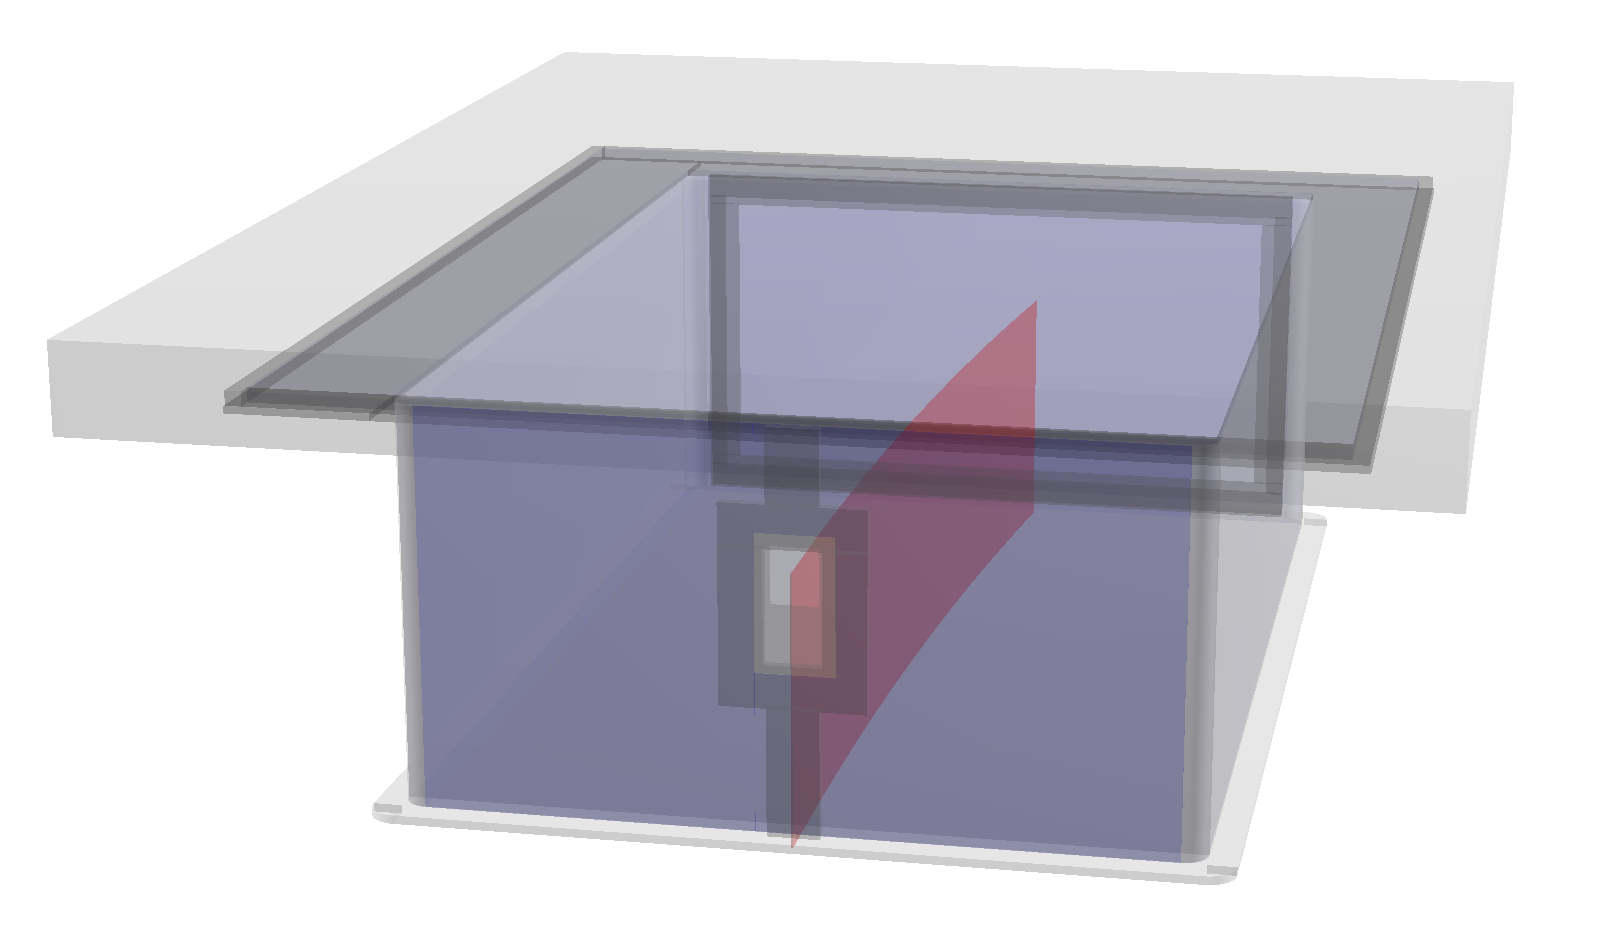
\includegraphics[width=\linewidth]{spacechg_cartoon.png}
\caption{Location of space charge in 132 Sn}
\label{fig:spacechg_cartoon}
\end{figure}


\begin{figure}[H]
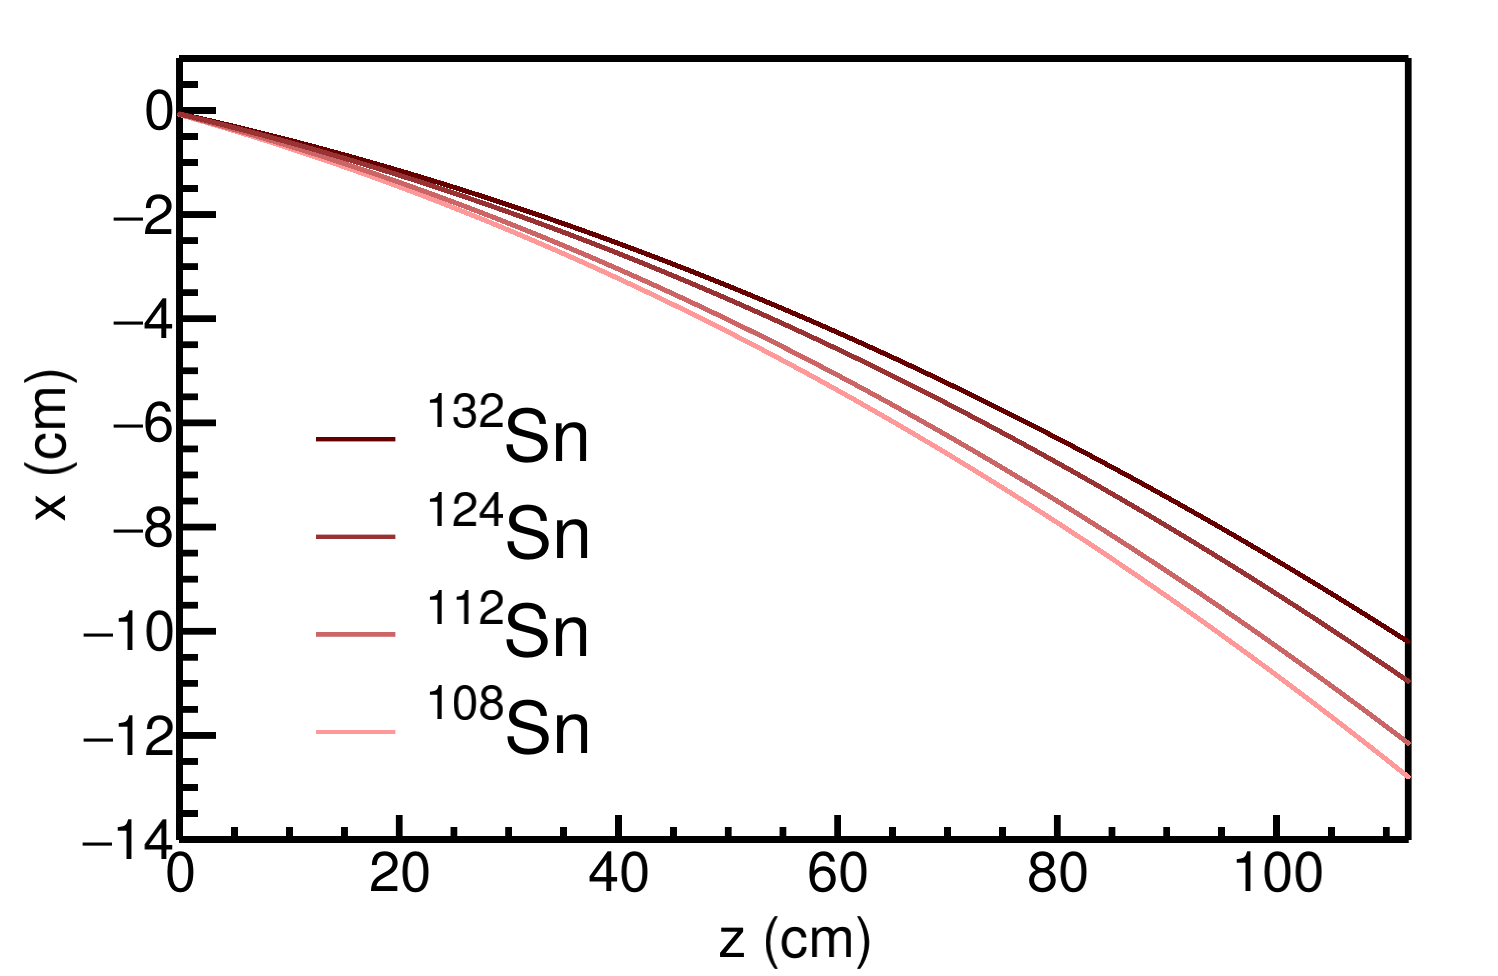
\includegraphics[width=\linewidth]{beampath.png}
\caption{Beam path of the experiments}
\label{fig:beampaths}
\end{figure}


As the beam passes through the field cage it ionizes the gas along the way creating electron-ion pairs. The drift velocities of the ions are \num{1e4} times slower than the electron drift velocities. Because ions move very slow, the potential build up of positive ions may create a space charge which distorts the drifting electrons of the tracks, impacting the measurement of their momentum. There are several regions of the TPC in which electron-ion pairs are created. The largest source of positive ions are created in the avalanche process near the anode wires. These ions slowly drift toward the cathode and are captured by the gating grid. The other source of ions come from the primary ionization produced by the beam and reaction products in the detector gas. The energy loss <dE/dx>$\propto Z^2$, where Z is the charge of the particle type. Because the charge of the un-reacted beam is around Z~50, the ionization due to the beam is a factor of \num{2.5e3} times that of the light charged particles which mostly are of charge Z~1. 
 The beam is positioned about 25\si{\centi\metre} below the anode plane in the TPC. It takes electrons approximately 5\si{\micro\sec} to drift to the anode plane. It takes the ions \num{5e4}\si{\micro\sec} to travel. The beam rate in the experiment varied around a value of about 10\si{\kilo\hertz}, which has an average occurrence of 1 beam every 100\si{\micro\sec}, which is much shorter than the time it takes for the ions created by each beam to terminate on the cathode plane. This results in a build up of positive ions in the shape of a sheet charge, carved out by the beam path as shown in Fig.~\ref{fig:spacechg_cartoon}. The average distance between sequential ion paths created by each beam is a spacing of about 50\si{\micro\metre} apart, and the average number of beam paths that compose the sheet charge is around 500 tracks. 
Though the arrival time of each beam track is random, the large number of tracks, and small inter beam spacing, allows us to approximate the sheet charge as an uniform sheet charge. 

The electric field in the presence of the sheet charge can be calculated by solving Poisson's equation, 

\begin{equation}
\nabla^2 \phi = \rho,
\end{equation}

 where $\phi$ is the electric potential and $\rho$ is the free space charge; given the Dirichlet boundary conditions of the field cage. The electric field is given as the gradient of the potential,  $\vec{E}= -\nabla \phi$. 
 
 To reduce computation time, we notice that $\vec{E}\propto \rho$, we can therefore solve the electric field for a reference free charge $\rho_o$ and scale the solution for any other free charge. The full magnetic field map is provided by the SAMURAI collaboration \cite{magnet}. The velocity field map is given by Eq.~\ref{eq:elecdrift} and the electron drift through this velocity map is propagated by using a time stepped $\mathrm{4}^{\mathrm{th}}$-Order Runge-Kutta integration. The correction map is calculated by starting from the anode y-position and the measured (x,z) on the pad-plane and stepping backward in time in the Runge-Kutta integration through the velocity field map until the electron reaches the measured y-position. 
 
 It has been shown before that the amount of space charge present in the chamber is related to observables such as the distance of closest approach of each track to the vertex point \cite{starSC}. This is easily understood, as the space charge distorts the electrons as they drift through the chamber eventually distorting the overall shape of the measured track. In the presence of no space charge, you would correctly expect the distance of closest approach of each track to the vertex point would be a distribution centered around zero. In the presence of space charge the tracks are distorted and the distribution has some mean bias. 

Shown in Fig.~\ref{fig:sc_shift} is an example of the distortion map in the TPC for left-going tracks in blue, and right-going tracks in green, with the vectors of distortion magnified. The space charge affects left and right going tracks differently, with the right-going tracks going to higher momentum values and the left-going tracks going to lower momentum values. The inset figure of Fig.~\ref{fig:sc_shift} shows the shift in the x-position distance to vertex for the displaced left-going track given by $\Delta\mathrm{V}_\mathrm{x}$, with the opposite direction for right-going tracks. We are able to measure the amount of distortion the space charge creates by measuring the difference between the most probable values of the left-going and right-going tracks which we define as $\Delta\mathrm{V}_\mathrm{LR}$, see Fig.~\ref{fig:VLR}.mom
 

Overview
Discuss the relevant time scales, drift lengths, magnitudes, and locations of space charge


\begin{figure}[H]
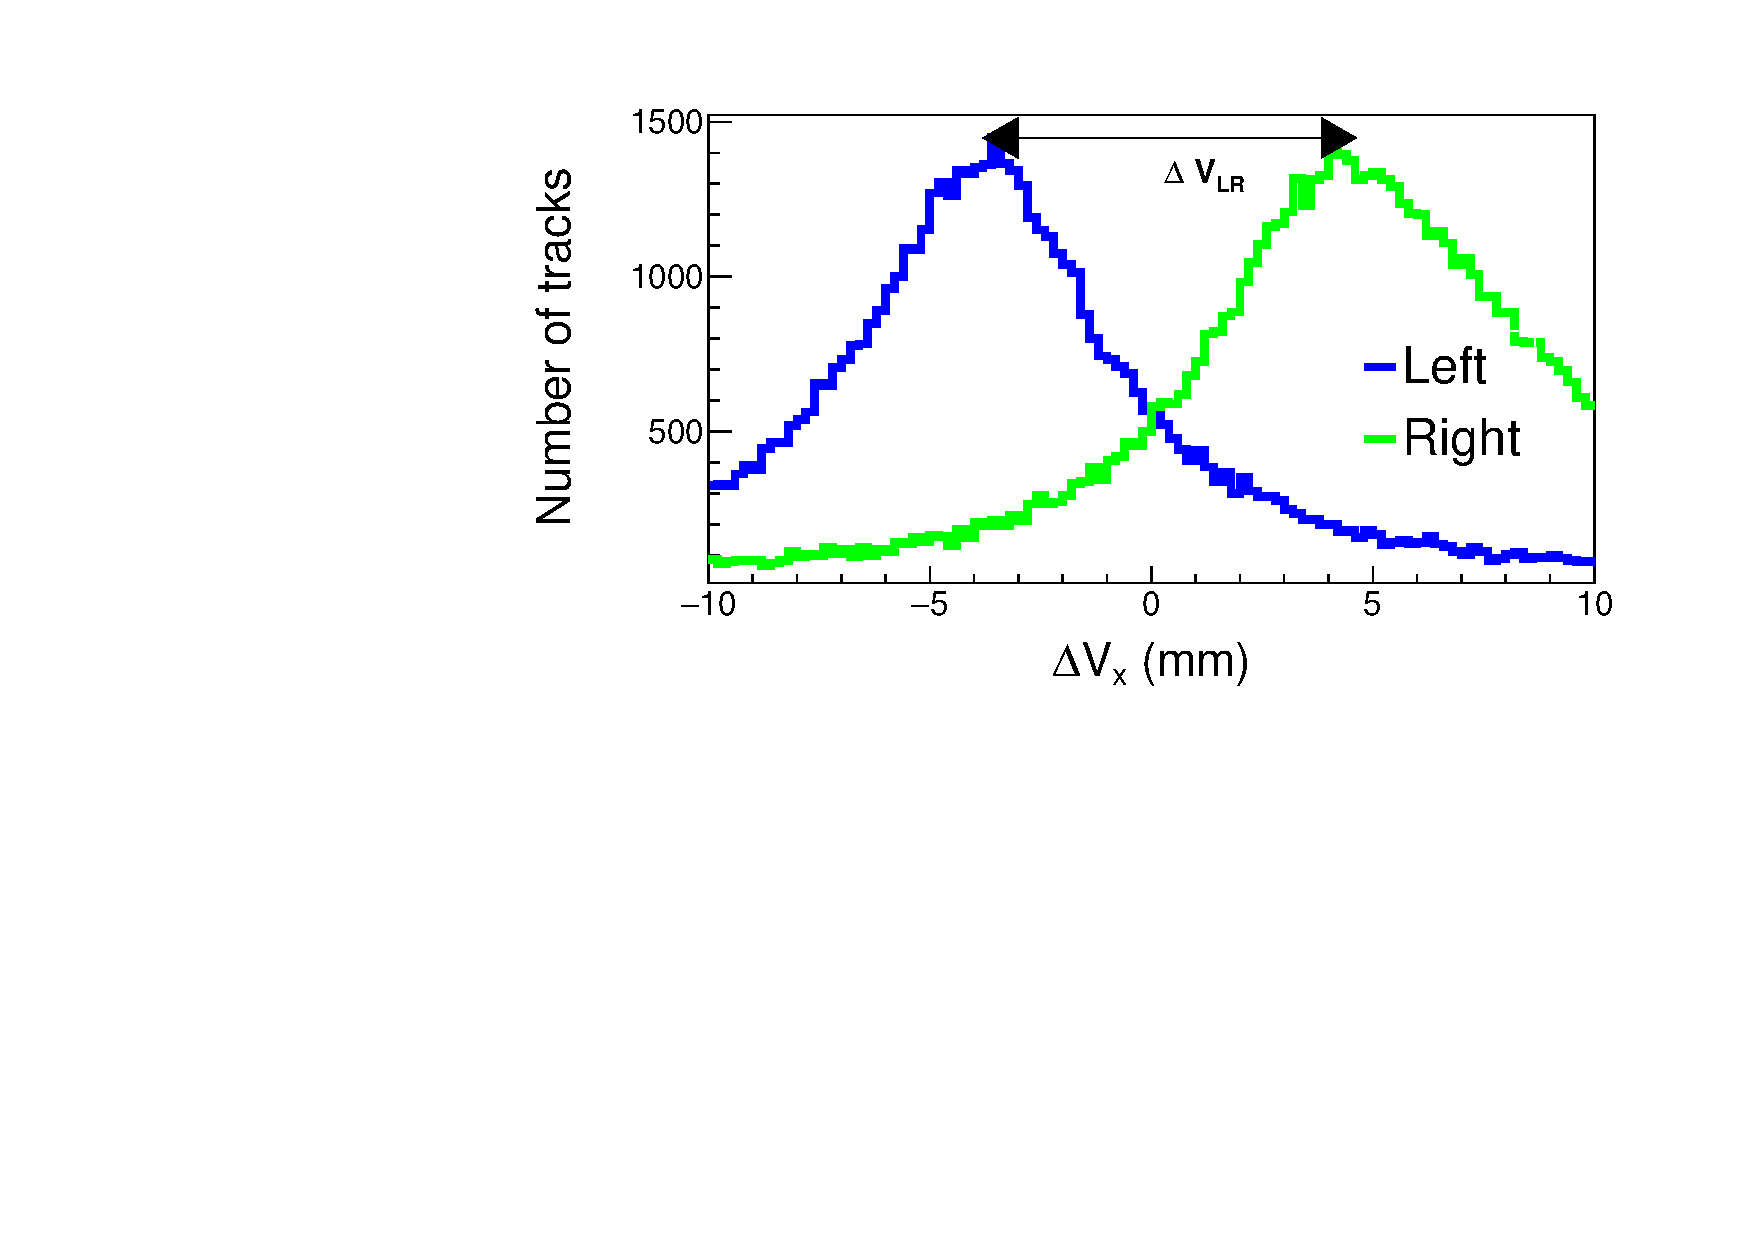
\includegraphics[width=\linewidth]{DVTP_raw.pdf}
\caption{$\Delta\mathrm{V}_\mathrm{x}$ distribution for left-going and right-going tracks in the TPC for the }
\label{fig:VLR}
\end{figure}


\begin{figure}[H]
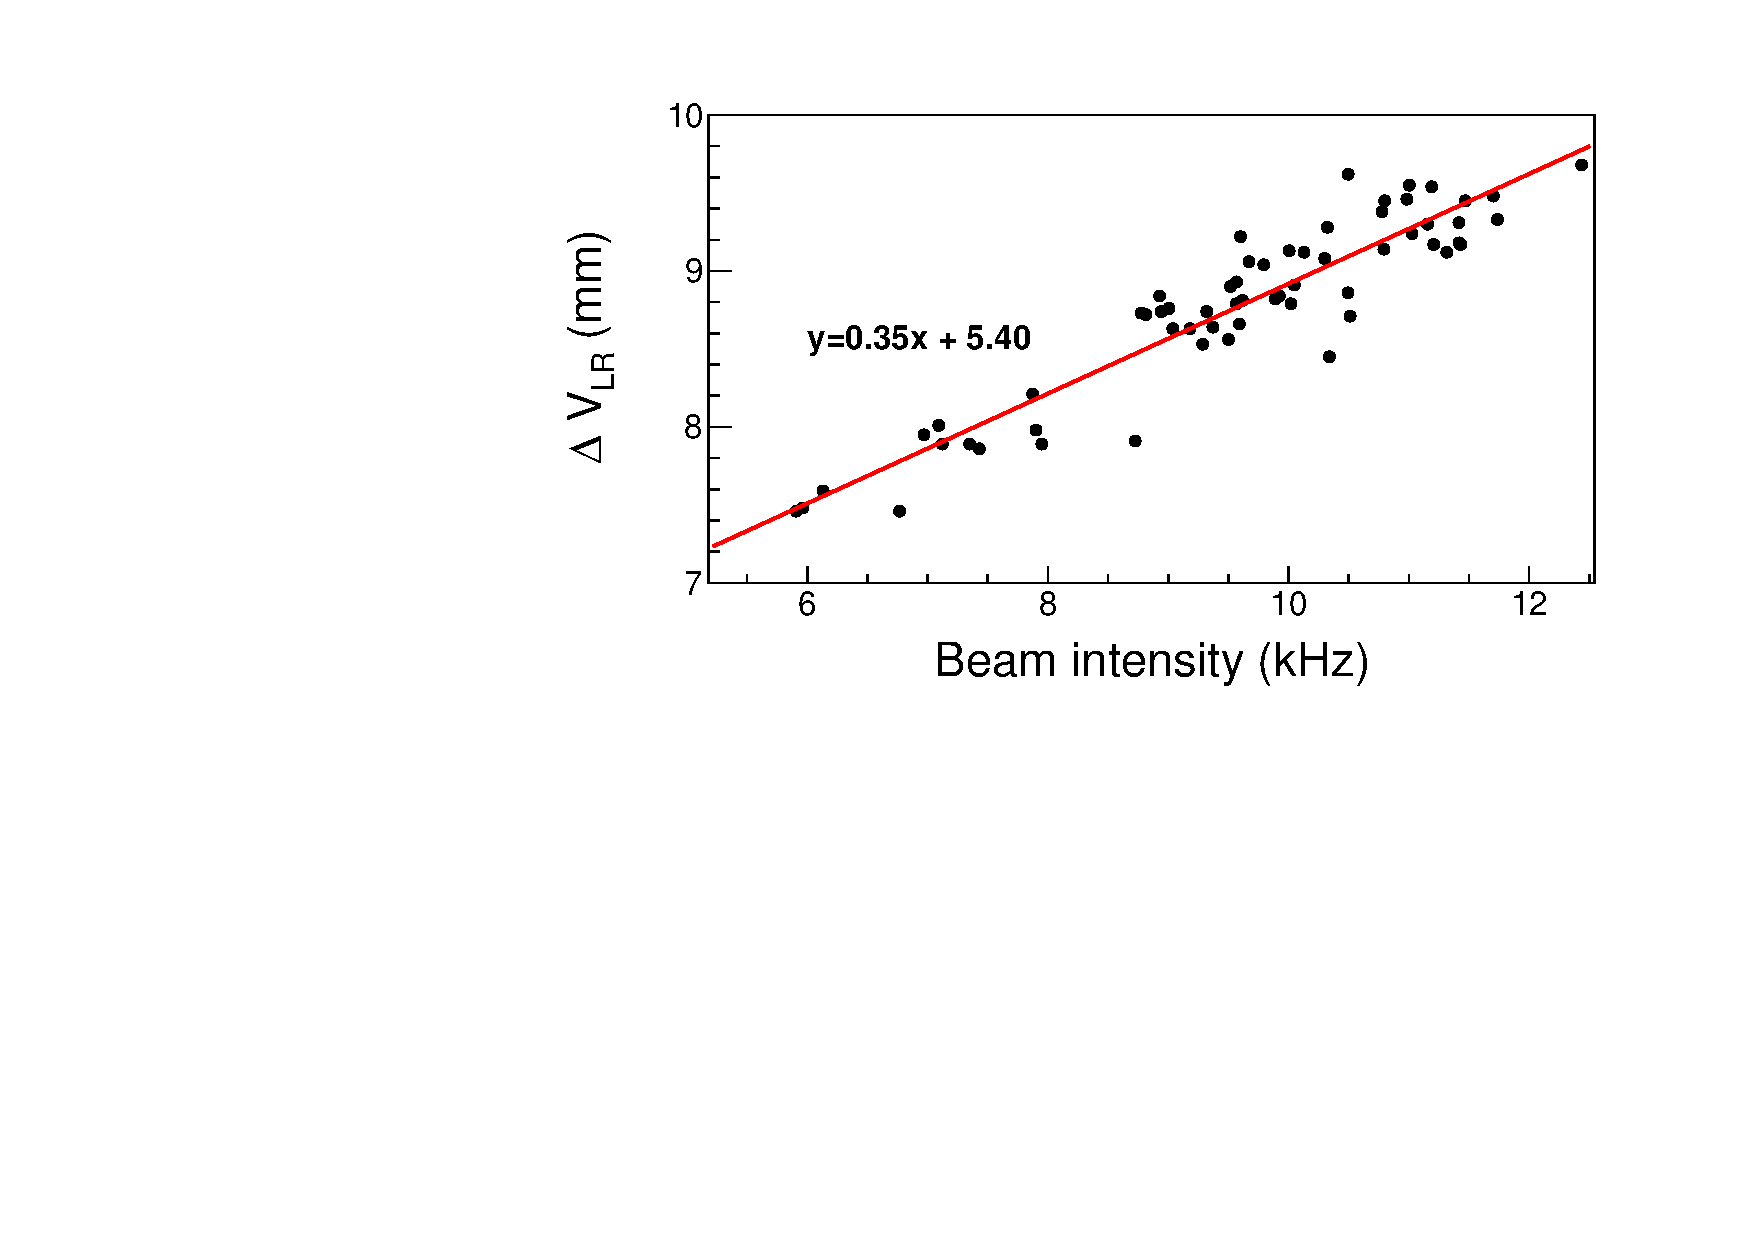
\includegraphics[width=\linewidth]{PeakLocation_vs_BR.pdf}
\caption{$\Delta\mathrm{V}_\mathrm{LR}$ as a function of the beam rate. }
\label{fig:spacechg_br}
\end{figure}

The average beam rate was recorded in each experimental run and slightly varied from run to run, due to beam production variations. The amount of space charge present in the field cage is directly proportional to the beam rate; therefore $\Delta\mathrm{V}_\mathrm{LR}$ is also proportional to the beam rate as shown in Fig.~\ref{fig:spacechg_br}. The only parameter in the space charge correction algorithm is the surface charge density $\sigma_{\mathrm{SC}}$. By varying $\sigma_{\mathrm{SC}}$ for a wide range of values the $\Delta\mathrm{V}_\mathrm{LR}$ observable is measured and plotted in the left panel of Fig.~\ref{fig:spacechg_relation}. The surface charge density which gives $\Delta\mathrm{V}_\mathrm{LR} = 0$ is taken to be the estimate for the average amount of space charge present. This is done for several runs which vary in beam intensity. Since the relation is linear between the surface charge density and the beam rate, a linear fit gives good agreement for interpolating the surface charge values as a function of beam rate, as seen in the right figure of Fig.~\ref{fig:spacechg_relation}.

This is done for all the systems. I NEED TO PUT THE ASSUMPTIONS of SPACE CHARGE SHEET DENSITY OF 132 108 HERE!!!

From the BDC tracking, the precise interaction point on target is known. Using this point greatly improves the momentum resolution of the track fitting, but there is a systematic shift when comparing the momentum value without using the vertex BDC point in the fit. The space charge affects right-going and left-going tracks differently making right-going tracks more rigid (higher momentum) and left-going tracks less rigid (lower momentum). For polar angles of $\theta < 40 \deg$, the disagreement between momentum values fitted with the BDC, versus without, are much less because the projection of the track does not disagree as much with the BDC point as tracks with polar angles of $\theta > 40 \deg$. This is seen in 


\begin{figure}[H]
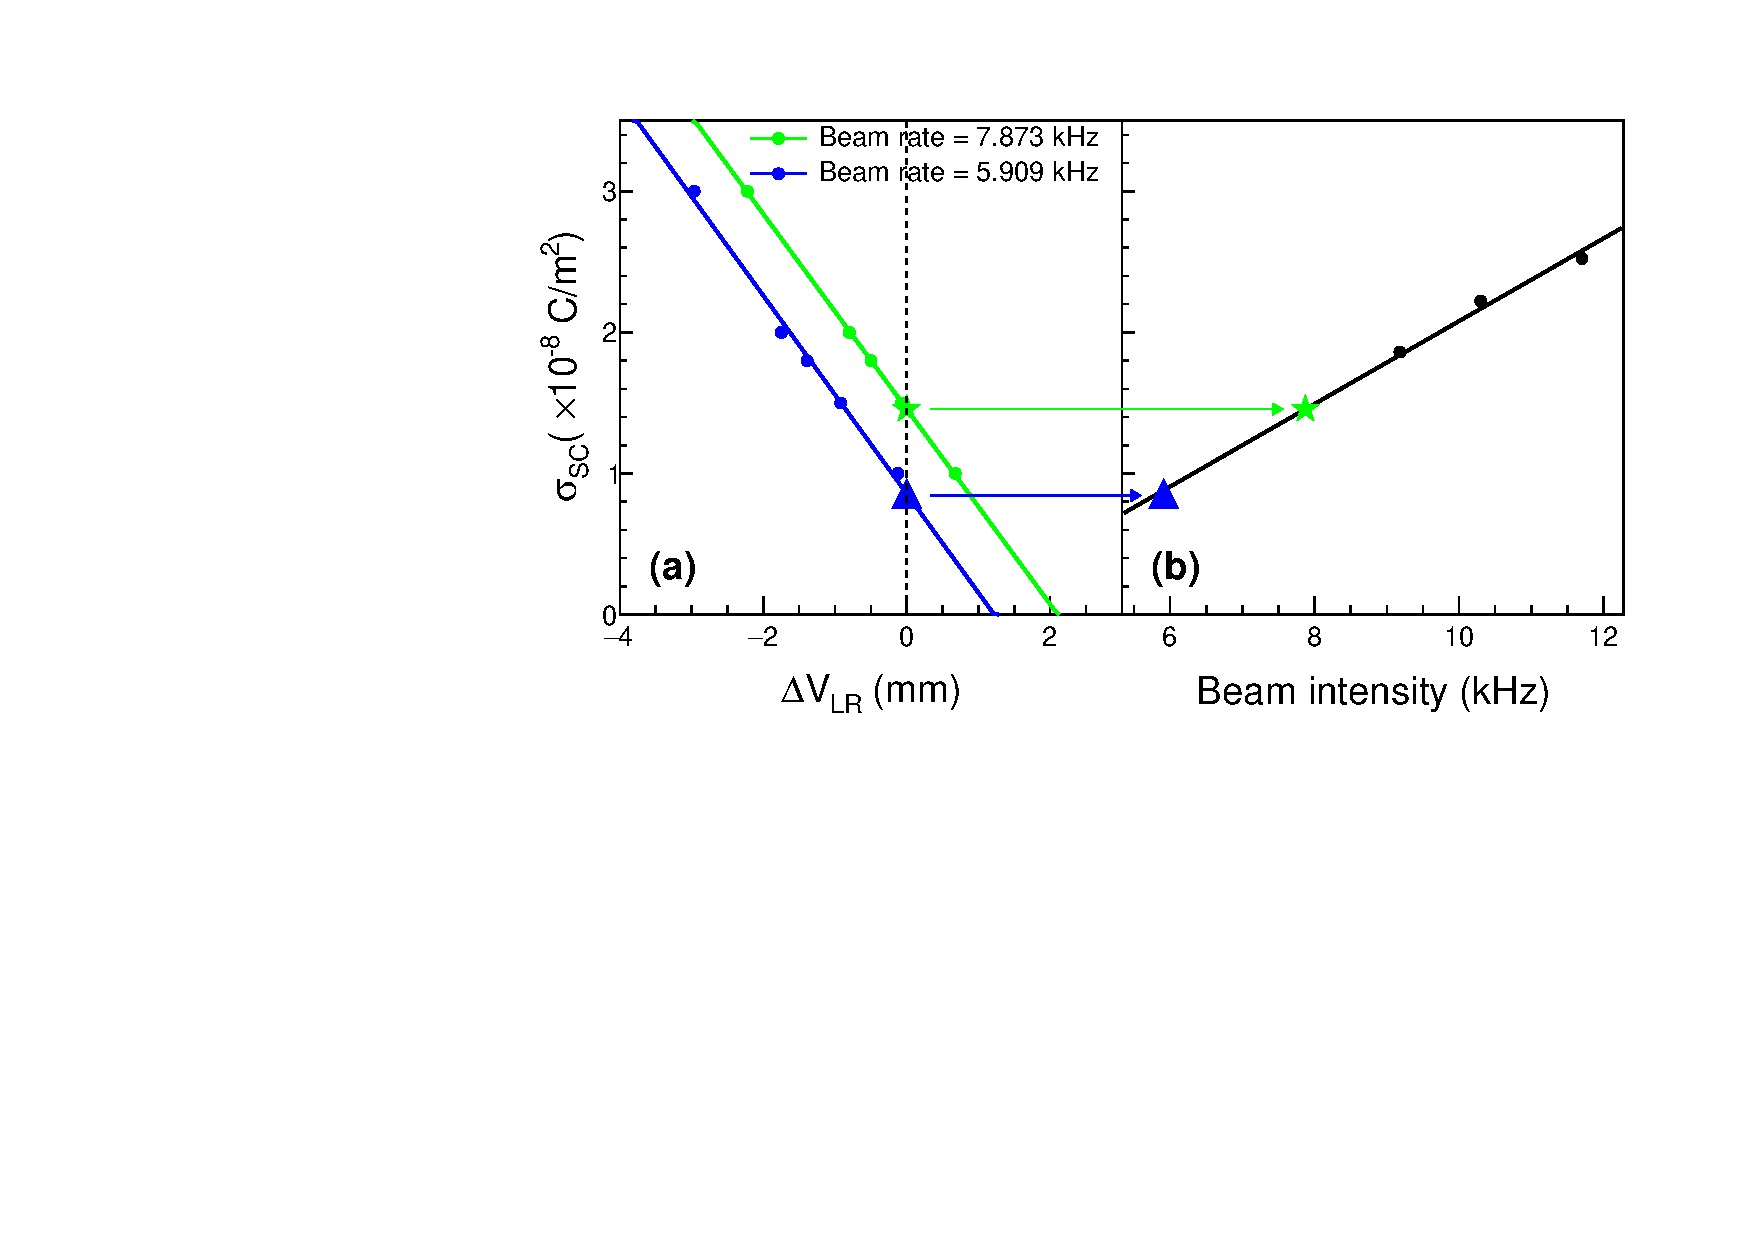
\includegraphics[width=\linewidth]{SC_Relation.pdf}
\caption{Space charge relation}
\label{fig:spacechg_relation}
\end{figure}


\begin{figure}[H]
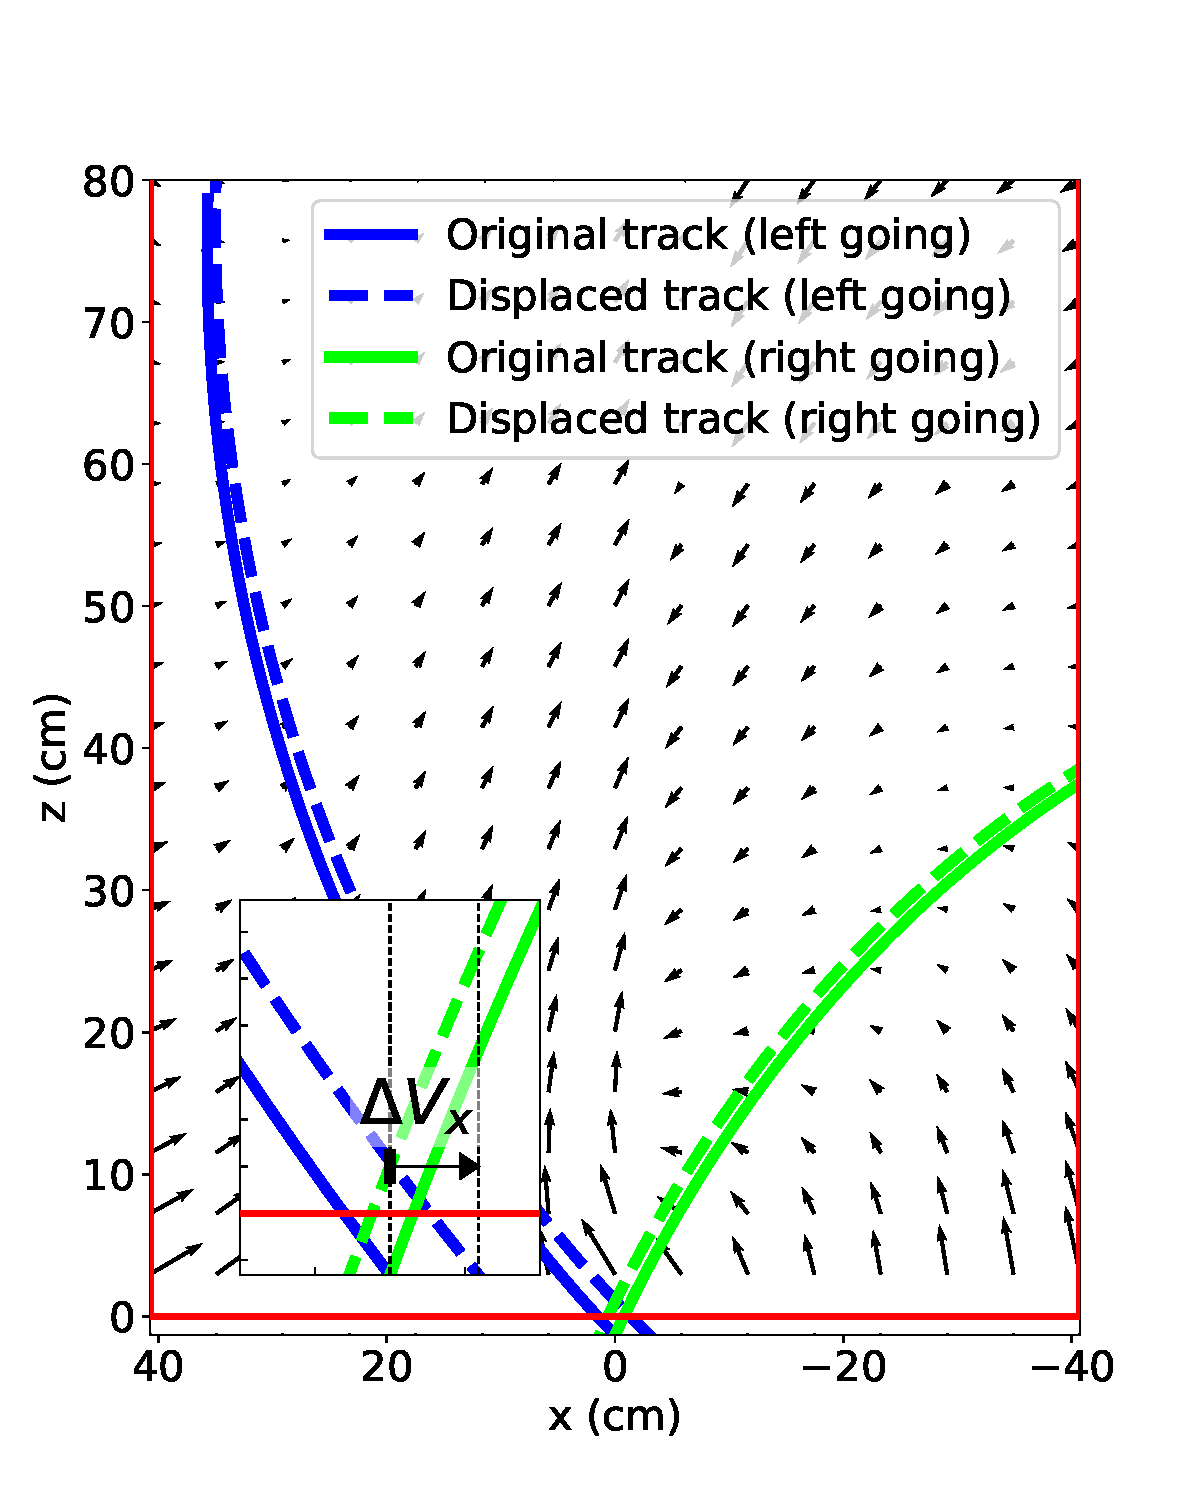
\includegraphics[width=\linewidth]{Effect_SC.pdf}
\caption{Shift of tracks}
\label{fig:sc_shift}
\end{figure}


\begin{figure}[!htb]
    \centering
    \begin{subfigure}[t]{0.45\textwidth}
        \centering
        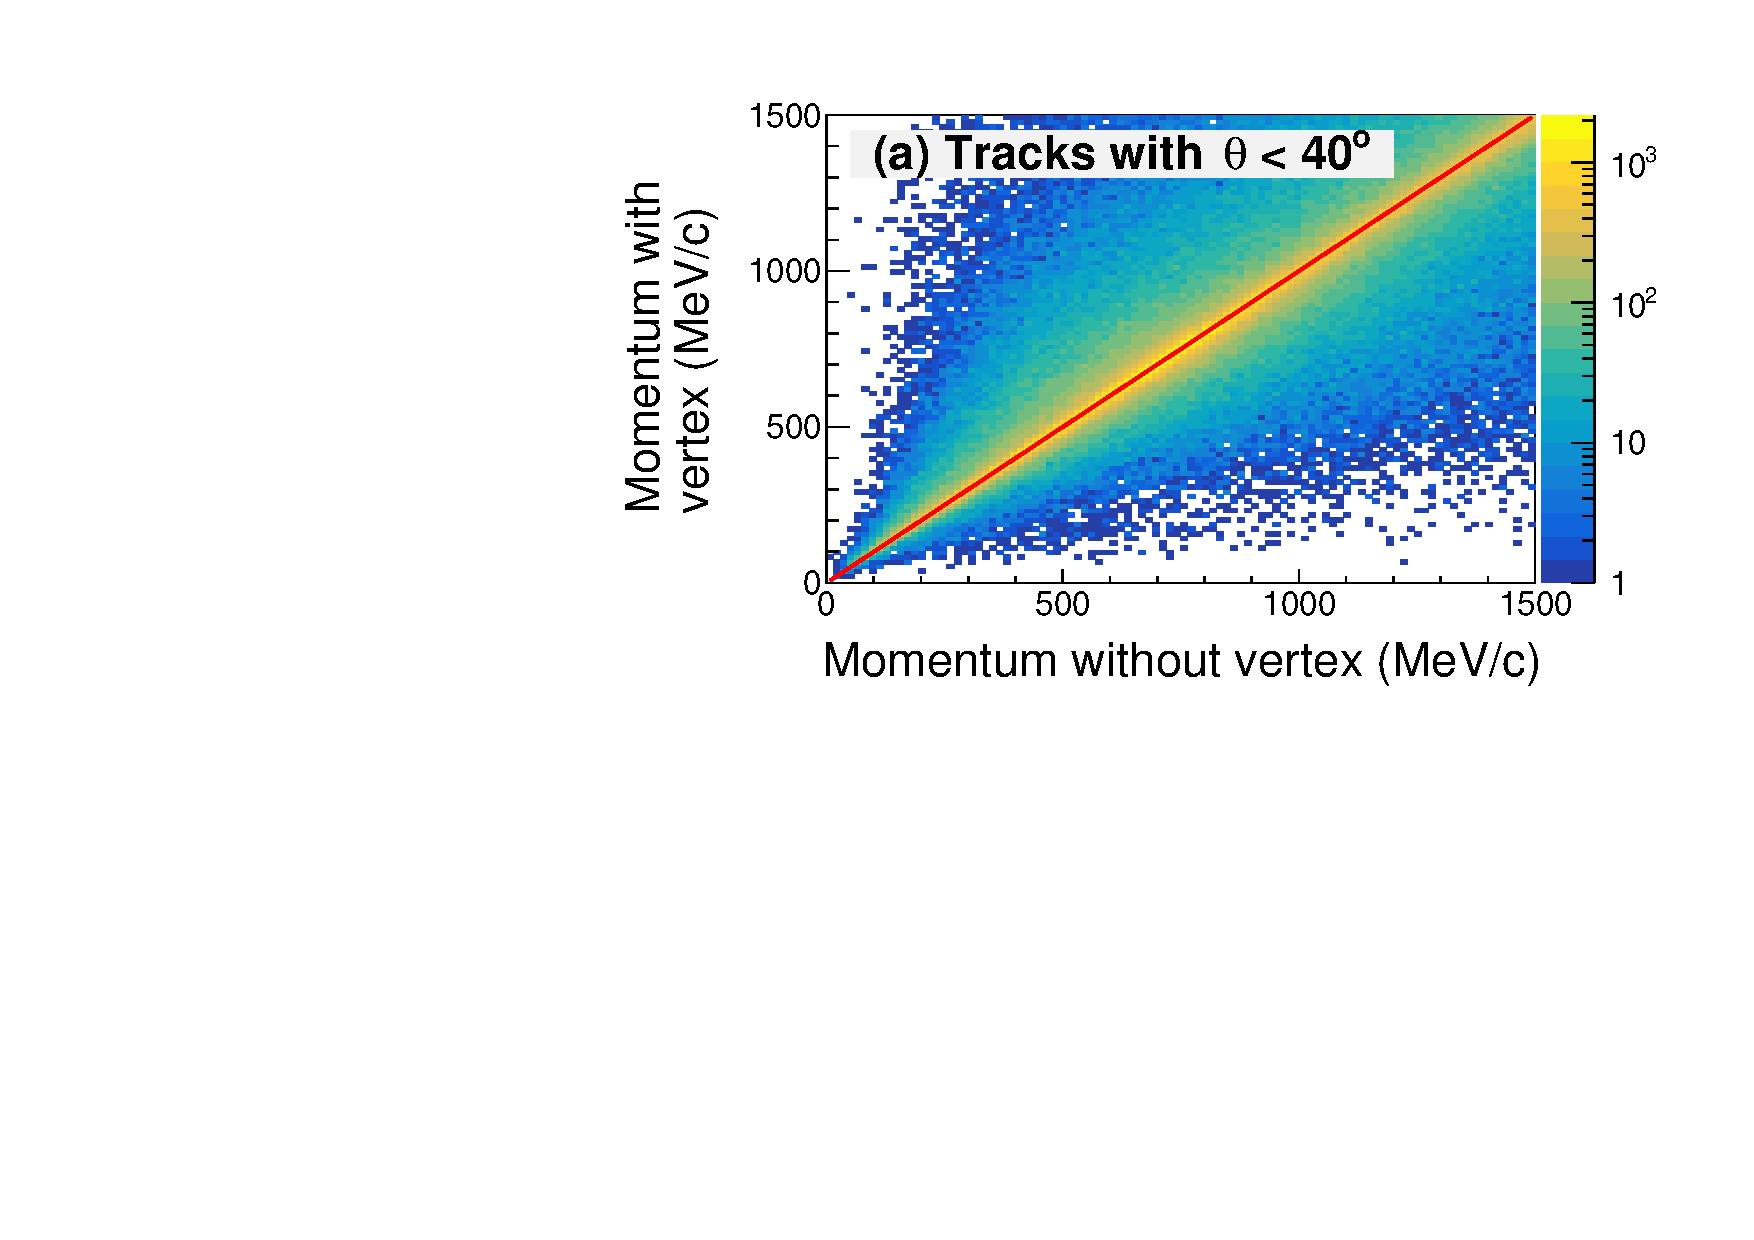
\includegraphics[width=\linewidth]{BDC_P_small_angle.pdf} 
        \caption{Generic} \label{fig:mom_S_before}
    \end{subfigure}
    \hfill
    \begin{subfigure}[t]{0.45\textwidth}
        \centering
        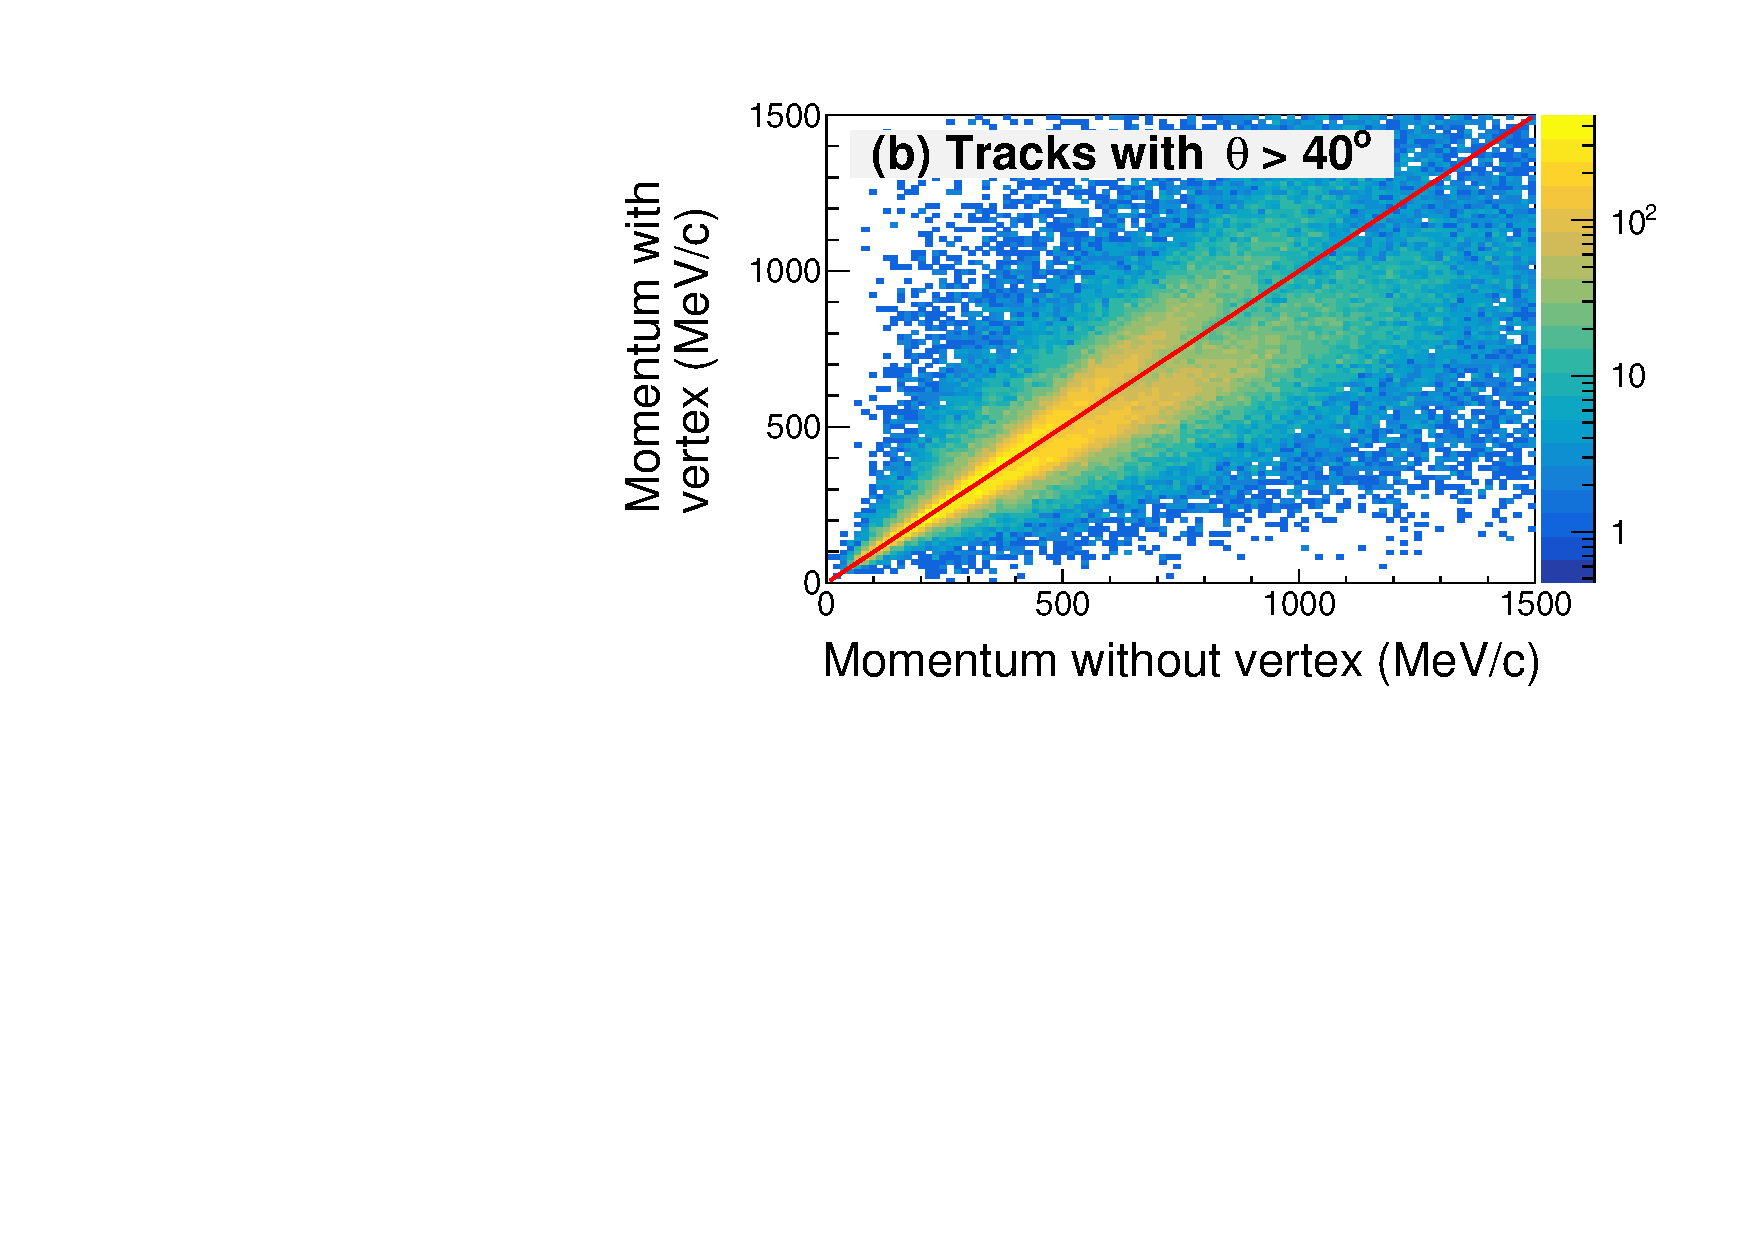
\includegraphics[width=\linewidth]{BDC_P_large_angle.pdf} 
        \caption{Competitors} \label{fig:mom_L_before}
    \end{subfigure}
    
    \begin{subfigure}[t]{0.45\textwidth}
        \centering
        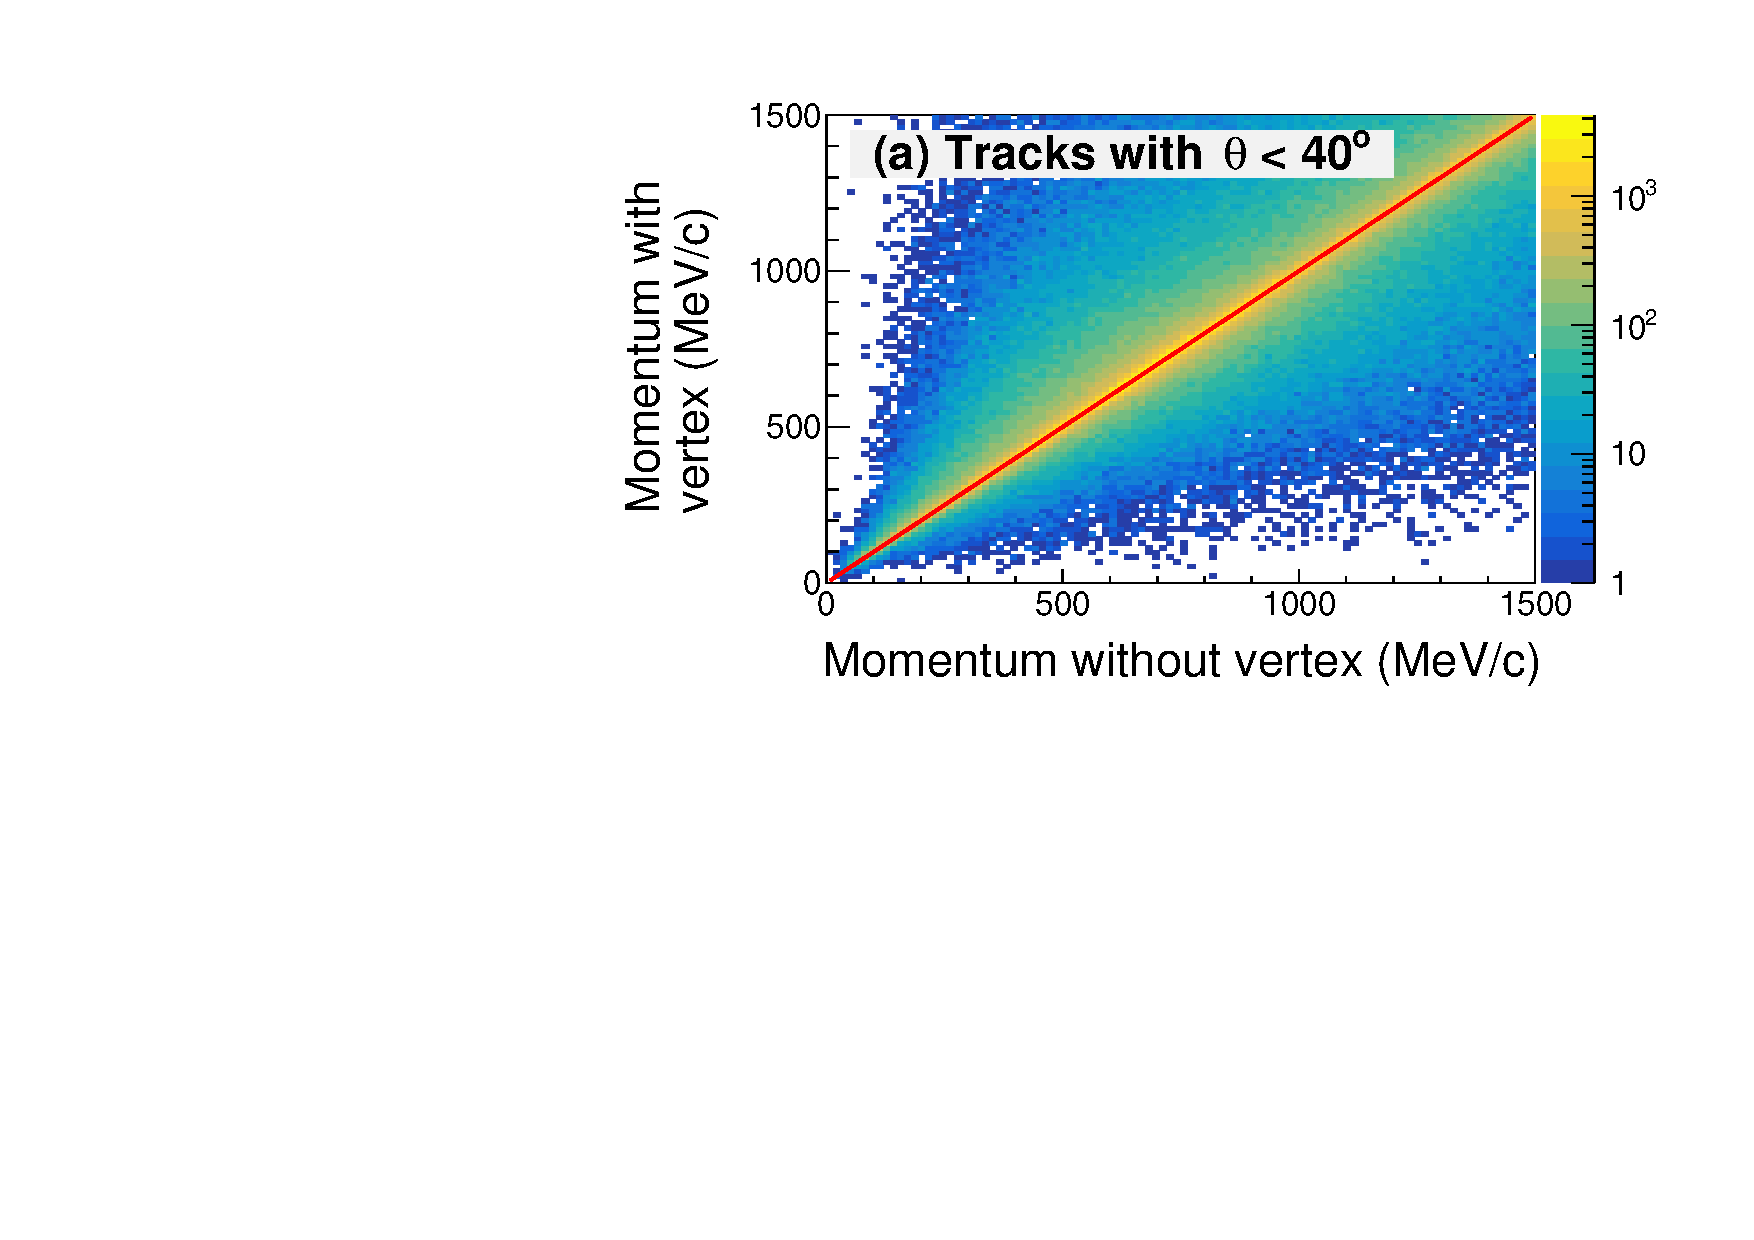
\includegraphics[width=\linewidth]{BDC_P_aftercor_small_angle.pdf} 
        \caption{Generic} \label{fig:mom_S_after}
    \end{subfigure}
    \hfill
    \begin{subfigure}[t]{0.45\textwidth}
        \centering
        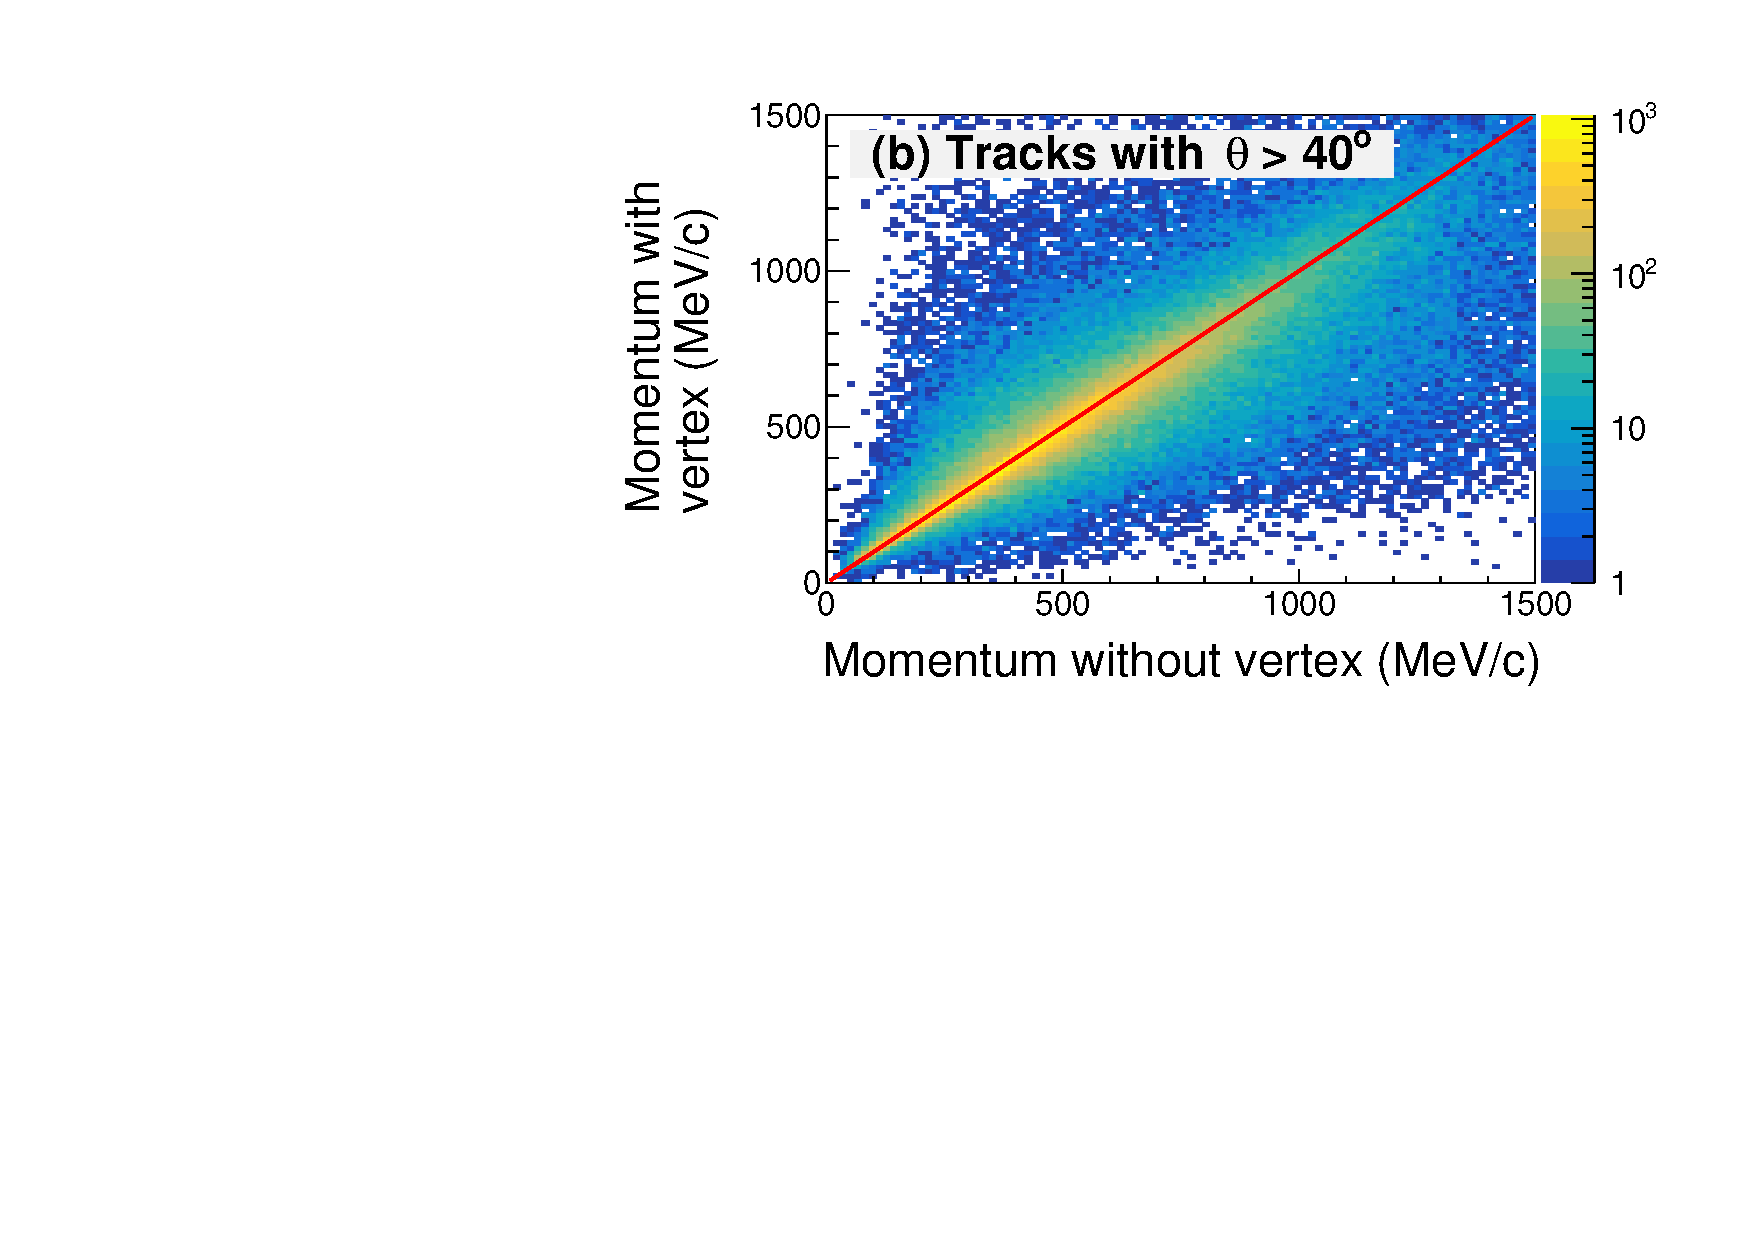
\includegraphics[width=\linewidth]{BDC_P_aftercor_large_angle.pdf} 
        \caption{Competitors} \label{fig:mom_L_after}
    \end{subfigure}
\label{fig:mom_sc}
\end{figure}



\begin{figure}[!htb]
    \centering
    \begin{subfigure}[t]{0.49\textwidth}
        \centering
        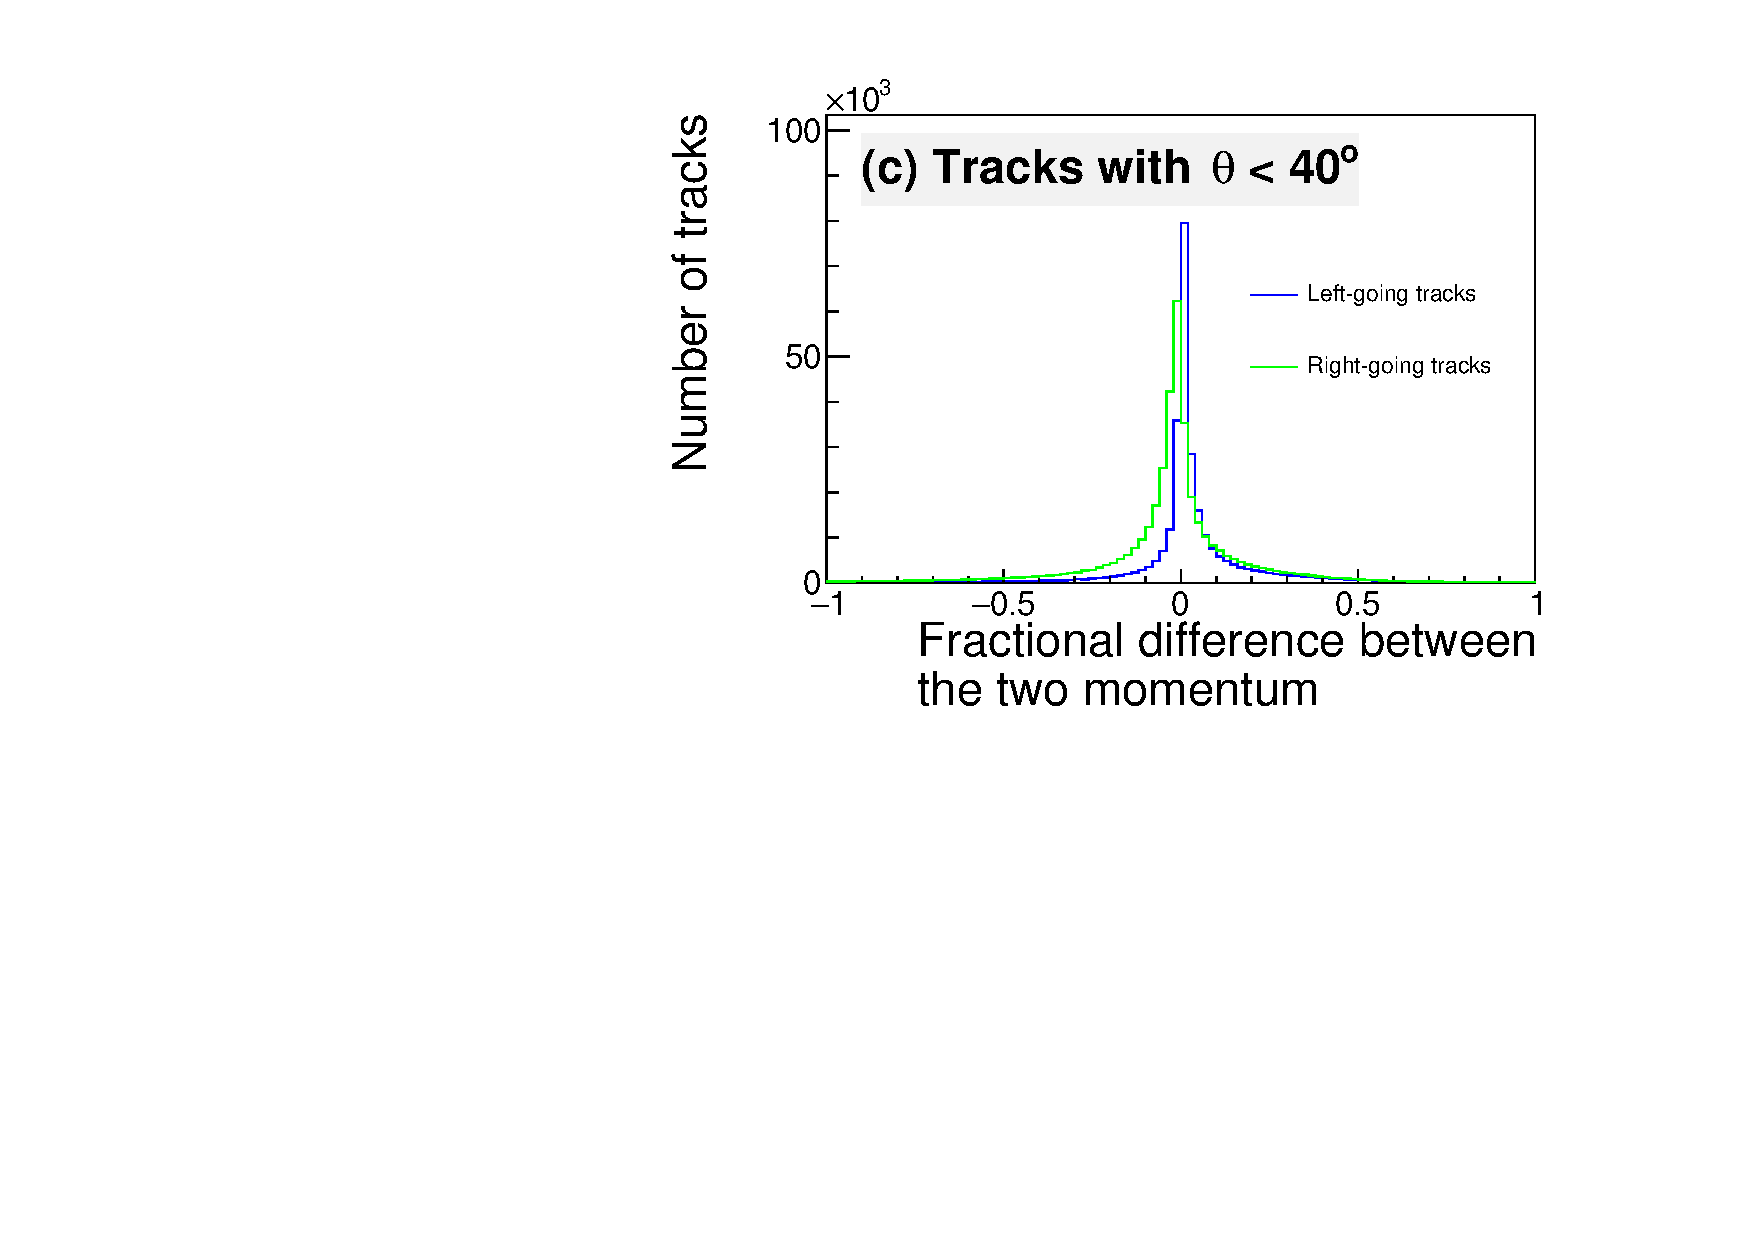
\includegraphics[width=\linewidth]{BDC_P_frac_small_angle.pdf} 
        \caption{Generic} \label{fig:mom_S_1D}
    \end{subfigure}
    \hfill
    \begin{subfigure}[t]{0.49\textwidth}
        \centering
        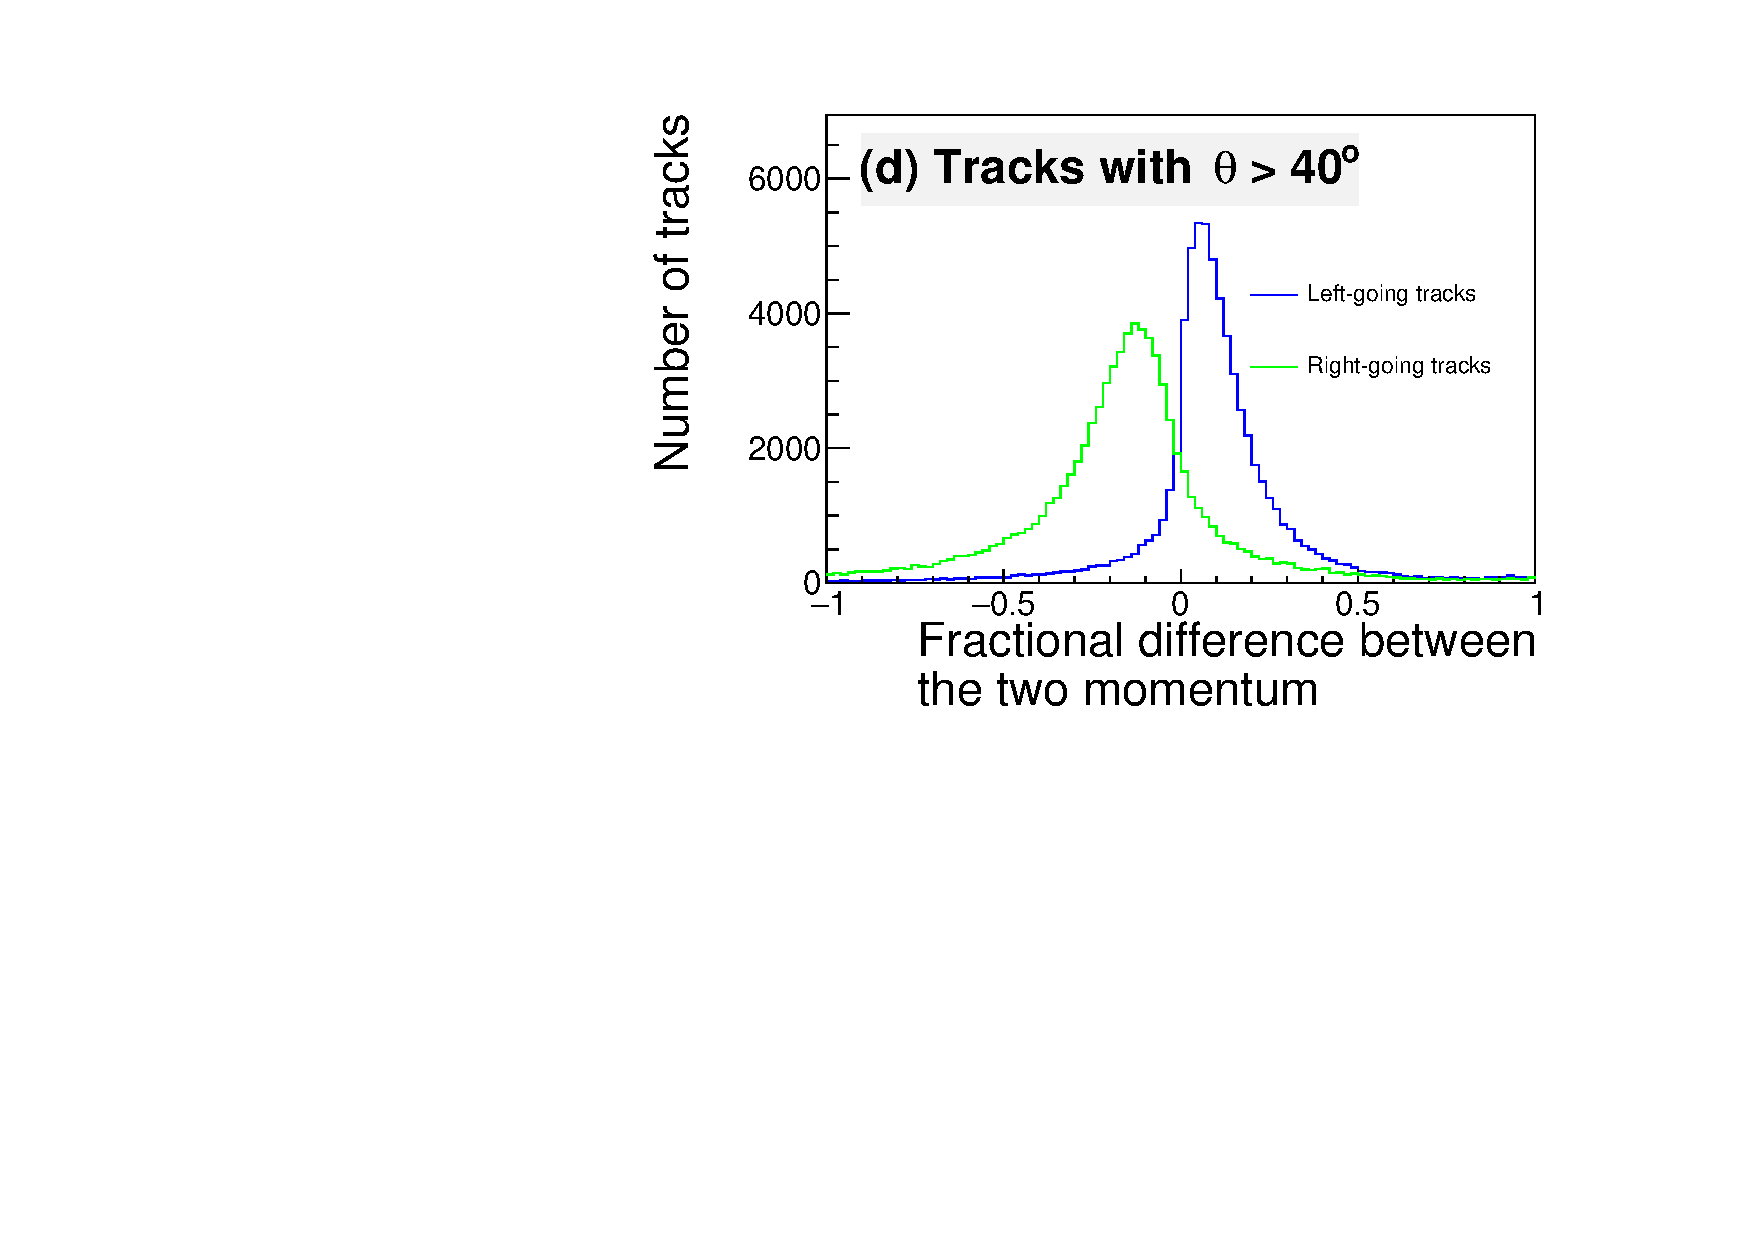
\includegraphics[width=\linewidth]{BDC_P_frac_large_angle.pdf} 
        \caption{Competitors} \label{fig:mom_L_1D}
    \end{subfigure}
    
\label{fig:mom_1D}
\end{figure}



Reference appendix for poisson solver 
Tables for ion drift velocity in P-10 Gas reference Sauli
Figure of sDAC or POCA 
Figure of cartoon of what is happening to tracks
Figure of correction map in TPC and MC map 
Figure of before and after correction BDC vs reco momentum
Figure of track residuals before and after?


In theory, a TPC functions with the electric and magnetic fields parallel to each other. In this way the electrons move opposite to the electric field winding tightly around the magnetic field lines, reducing transverse diffusion in the process. In practice, due to the finite size of the dipole magnet and field cage, there are traverse components to both the electric and magnetic fields. These transverse components introduce drift velocities in the transverse directions, causing a shift in the measured cluster positions of the track. Thereby introducing systematic shifts in the calculation of the momentum and the vertex calculation. 

Most of the time the beam does not undergo a nuclear collision with the target and passes through the TPC drift volume. The KATANA array threshold was set to veto such events, ensuring the gating grid remain closed to prevent the large amount of charge deposited by the beam into the avalanche region. While the electron drift velocity is fast enough for the electrons produced by the unreacted beam to terminate on the closed gating grid, the drift velocities of the positive ions produced are of order $10^{-4}$ times slower. At higher beam rates the positive charge is allowed to pile up producing a region of positive space charge, introducing perturbations to the nominal electric field. 

Since the beam comes in along the z-axis, and the drift direction of the ions is in the -y direction, we can estimate the charge density as an uniform sheet charge. The surface charge density is related to the beam rate, ion drift length, ion drift velocity, and the energy loss of the beam. Though the incoming beam comes randomly, the slow drift velocity combined with the high beam rate makes the uniform approximation valid. Tracking or estimating the beam rate as a function of time with in a given run would provide a better estimate of the space charge. Or experimentally a laser system could be pulsed after each event (throughout the drift volume), giving the experimental correction map for the drift. While the potential for a laser system was implemented in the field cage design, a laser system ultimately was not developed for the \spirit tpc. 

The beam rate within a run is roughly constant, therefore we can estimate the space charge and provide a first order correction for the space charge effect. 

As mentioned in CHAPTER ???, the cocktail beam momentum was well known to within 1\% as set by the BIGRips spectrometer. Also time of flight analysis of upstream and downstream scintilators also independently confirmed the beam rigidity setting. The expected momentum is given in TABLE ??? as calculated by from the beam rigidity setting of the magnet (WHICH MAGNET). The measured momenta as determined by the TPC software (given in FIG TABLE ), shows a disagreement on the level of 5\% too high. We noticed that if one only uses the first 90 layers (out of 112) of the TPC, the momenta is lower; one should expect the momentum to go higher as the track length is shorter (short tracks effectively are straight lines). 
In the cocktail beam there is no un-reacted beam causing any significant space charge. The magnetic field map of the SAMURAI magnet has been calculated by TOSCA simulation CITE ???, and several points have been verified experimentally with a hall probe to be within XXX \%. We assume that the electric field (to first order) is uniform in the y-direction. Using Garfield++ CITE ???, we can model the transverse drift of the electrons in the presence of such fields. 

A grid of electrons uniformly distributed in the TPC model space were drifted to the gating grid position. The final shifts in the x and z positions was measured. 


\section{Monte Carlo Simulation}
The monte carlo (MC) simulation is a to part simulation. The first is the modeling of the fundamental interactions of a particle through material which we utilize Geant4 as an event generator. A scale model of field cage, front window, front window frame, pad plane, and aluminum top plate are modeled with the correct material type and dimensions assuming P-10 gas at a density of 1 atm. We also import the the magnetic field map of the SAMURAI dipole magnet (as calculated by the SAMURAI group via a TOSCA simulation) \cite{magnet}.  In this way any particle type may be studied and the full interactions (scattering, decay, energy loss, path taken, etc.), are accounted for. The output of this simulation is a series of energy loss points which contain the amount of energy lost in $keV/cm$ and the position in $(x,y,z)$. The second part of the MC simulation simulates the physical processes involved in the measurement of the TPC such as the drift, avalanche, and signal creation in the electronics, to simulate the detector response of the MC event. This is separated into several software tasks; the drift, pad response, and electronics task. 

Here we will only discuss in detail, the tasks involved in simulating the TPC response. The discussion of how we use Geant4 is not particularly interesting, since we use it only to get the energy loss in a gas and through basic materials. 

\begin{figure}

\includegraphics[scale=.01]{place}
\caption{A summary of all the effects modeled in the TPC MC simulation.}
\label{fig:place}
\end{figure}

\subsection{Drift Task}
Geant4 returns the primary ionization points and energy loss information in the gas volume. In the drift task this is converted into the total number of electrons, $N_{e^-}$,

\begin{equation}
N_{e^{-}} =  \frac{\Delta E}{I},
\label{eq:kev2el}
\end{equation}
 
where the ionization coefficient of P10 gas, $I$, given in Table~\ref{tb:gas} and the energy loss, $\Delta E$, given in \si{\electronvolt}.Since the electric field set up by the field cage is uniform for the area covered by the pad plane, we assume also each electron drifts in a straight line trajectory until reaching an anode wire, where the total length drifted is given by $L_{anode}$. In this task the option to put in space charge effects and non-uniform electric fields are allowed but we do not use them for the further discussion of calculating efficiency. 


\begin{table*}\centering
\ra{1.3}
\begin{tabular}{@{}rr@{}}\toprule 
\multicolumn{2}{c}{Electron Transport Gas Properties} \\
 \midrule
Drift velocity & 5.53 $\si{\centi\meter\per\micro\second}$\\
Transverse diffusion & 240 $\si{\micro \meter \centi\meter}^{-1/2}$\\
Longitudinal diffusion &  340 $\si{\micro \meter \centi\meter}^{-1/2}$\\
Gas Ionization & 26.2 $\si{\eV}$\\
\bottomrule
\end{tabular}
\caption{An overview of the properties of the TPC}
\label{tb:gas}
\end{table*}

The drifting electrons exhibit stochastic motion which can be described by a longitudinal, $c_{l}$, and transverse, $c_{t}$, diffusion coefficients, which are determined by Garfield++ calculations -- in the presence of a 0.5T magnetic field. The diffusion of electrons can be modeled by randomly sampling from a Gaussian distribution in both the longitudinal and transverse directions of the electron drift. The stochastic deviation in the transverse direction, $dr$, can be randomly sampled from,

\begin{equation}
dr = e^{-\frac{r^2}{2\sigma_{t}^2}},
\end{equation}

where $\sigma_{t}=c_{t}\cdot\sqrt{L_{anode}}$.The Cartesian directions are given by $dx = dr \cdot \cos(\alpha)$ and $dz = dr \cdot \sin(\alpha)$, where $\alpha$ is a random angle from 0 to 2$\pi$, as there is no preferential angle in the transverse directions. The longitudinal diffusion is simulated in the same manner by randomly sampling from, 

\begin{equation}
dt = e^{-\frac{t^2}{2\sigma_{l}^2}},
\end{equation}.

where $\sigma_{l}=c_{l}\cdot\sqrt{L_{anode}}$. 

The total drift time, $t$, is calculated as,

\begin{equation}
 t = L_{anode}/v_d + dt + t_{offset},
\end{equation}
 
 where $v_d$ is the drift velocity and $t_{offset}$ is an offset parameter added to align the MC time bucket spectrum with the data. The electron is assumed to terminate on the nearest anode wire which will fix the z-position to be the same as the that anode wire. 

The total number of electrons produced in the avalanche process of a single electron was simulated in Garfield++, Fig.~\ref{fig:gaincalib}. Two anode wire voltages were applied which correspond to two different anode gains, high and low, in the TPC experiment. We randomly sample from these two distributions, depending on which anode wire section the electron terminated on and store the number of electrons as an effective gain value. We do not assume there is much lateral movement along the wire in the avalanche process. 

\subsection{Pad Response Task}
The total charge of the event is split over several pads defined by the PRF, as discussed in section \ref{sec:prf}. We simulate the PRF as the double integral of a 2-dimensional Gaussian with the final output charge on each pad being the superposition of the PRFs of all drifted electrons. The MC PRF is expressed as, 

\begin{equation}
PRF(x,z) = \iint e^{-\frac{(x-x_o)^2}{2\sigma_x^2}} e^{-\frac{(z-z_o)^2}{2\sigma_z^2}}dxdz,
\end{equation}

where $\sigma_x = 3.4$ and $\sigma_z = 3.5$, and $x_0$ and $z_0$ are the final position of the drifted electron. The $\sigma$ parameters were determined through an iterative comparison between the MC and experimental data set. We can see good agreement between the MC PRF for $\pi^-$ in Figure~\ref{mcdataPRF}, and the data PRF, Fig.~\ref{prfpimData}, where the black line is the PRF fit to the experimental data.

\begin{figure}[!htb]
         \centering
         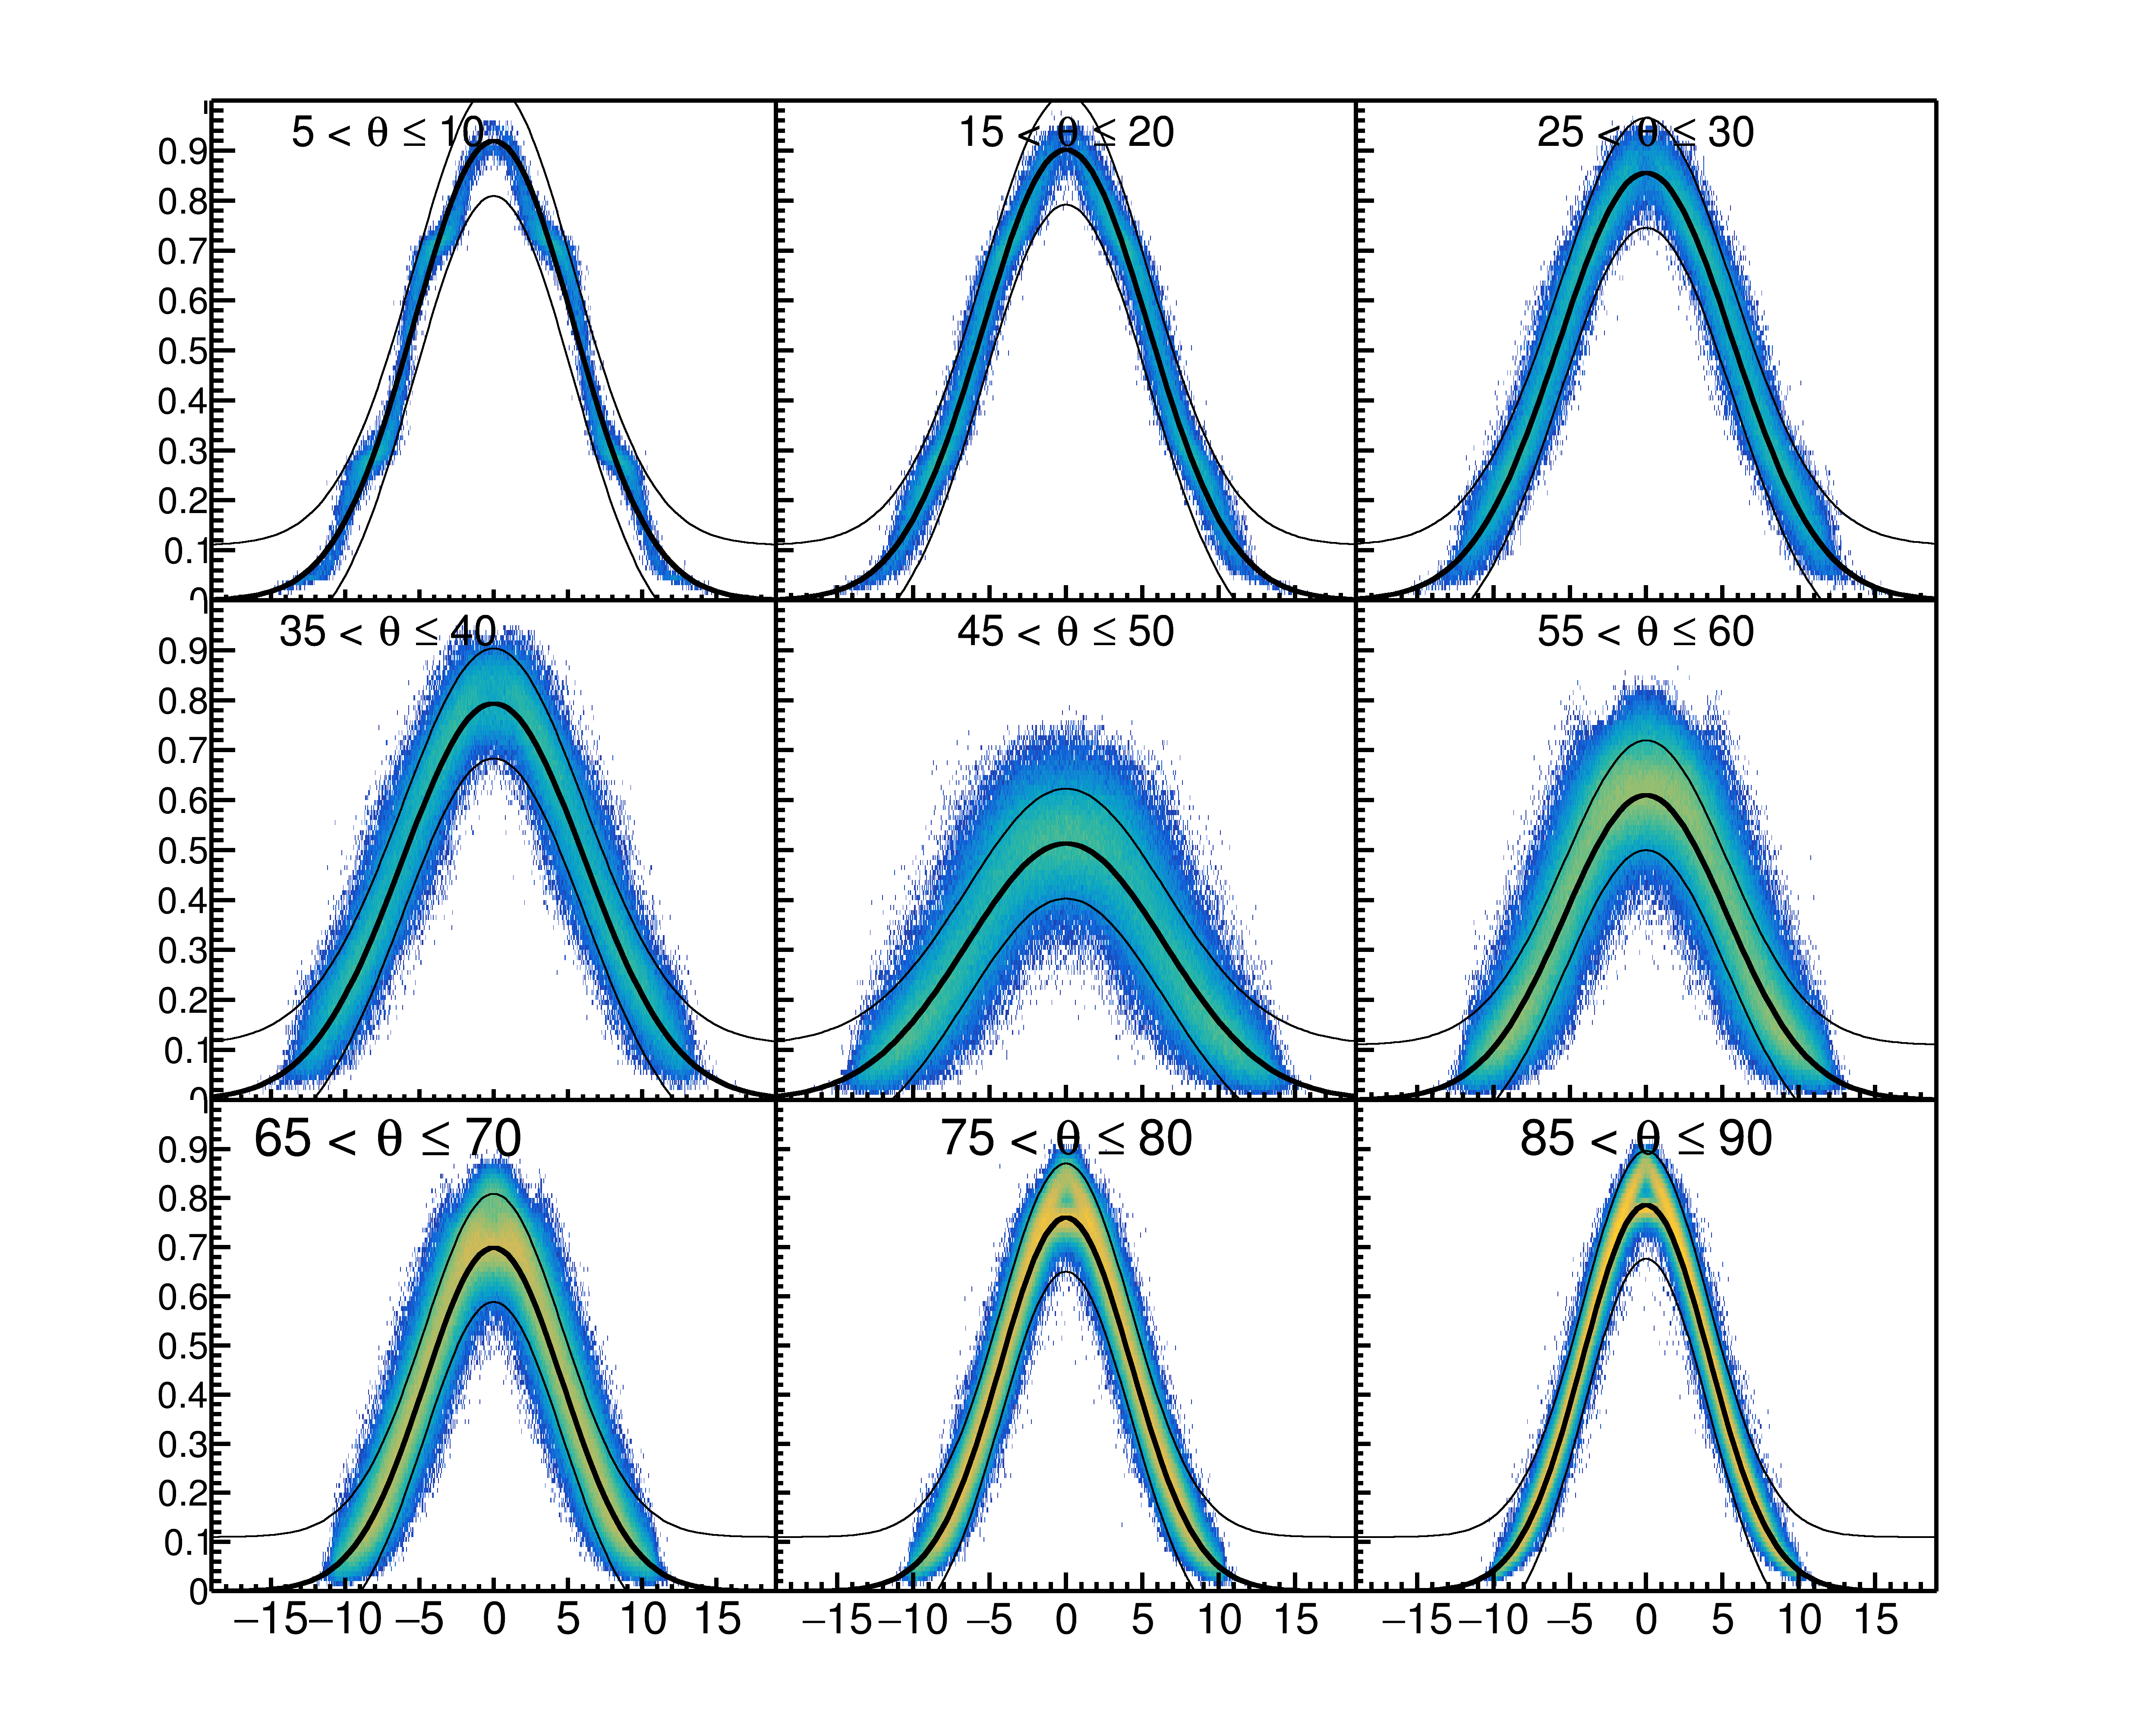
\includegraphics[width=\textwidth]{PRFs_MC_wcut.png}
         \caption{PRF response of Monte Carlo simulation of $\pi^-$}
         \label{fig:prfpimMC}
\end{figure}



\subsection{Electronics Task}
%The dynamic range, $d_{range}$, of the TPC electronics was set to 120 $\si{\femto \coulomb}$ over the full 12 bit resolution resulting in 4096 channels, $ADC_{max}$. The pedestal ($ADC_{pedestal}$) was set to 300 channels. The response of an electronics signal is simulated by measuring the standard pulse response to an input signal in the data. It was found the pulse shape did not depend on the momenta, angle, or particle type in any significant way. Therefore a standard pulse was extracted from an average over all particle types and signal heights -- as long as it were not saturating-- shown in Fig.~\ref{fig:pulsea}. The superposition of the individual pulses from each electron makes up the Monte Carlo (MC) time bucket spectra in ADC. This can be directly fed into the software. The experimental electronic noise (RMS) was measured to be around 6 ADC; a random number --drawn from a Guassian with a sigma of 6 ADC and 0 mean -- was assigned to each time bucket to simulate the experimental noise. 


The electronics task simulates the electronics response, converting  the induced charge on a pad into ADC channels. The conversion from number of electrons to the response, $R$, in ADC channels is calculated as, 

\begin{equation}
R = A_{tot} \cdot e \cdot\frac{ADC_{max} - ADC_{pedestal}}{f_c}
\label{eq:etoADC}
\end{equation},

where $e$ is the typical charge of an electron in $\si{\femto \coulomb}$, $A_{tot}$ is the total number of avalanche electrons, $ADC_{pedestal}$) is the pedestal (300 ADC, $\mathrm{ADC_{Max}}$ is the maximum allowed ADC value (4096), and $f_c$ is the dynamic range setting (\SI{120}{\femto\coulomb}). We add random Gaussian noise as measured from the experimental simulating the electronic noise; (RMS) was measured to be around 6 ADC. 

The induced current in the pad goes through a pre-amplifier and shaping amplifier which determine the final pulse shape that is read out. The pulse shape did not change significantly in any circumstance, such as pulse height, data type, or particle type, for a given shaping constant. This allows us to assume the pulse shape is constant with the only two variables being the height of the pulse, $Q$, and the starting time bucket of the pulse, $t_o$. The shaping constant was set to \SI{117}{\nano\second} for the data analyzed here. Figure~\ref{fig:pulseshape} shows the pulse shape experimentally extracted from signals that did not saturate the electronics over a wide range of ADC values; it is normalized so the maximum height is 1. 



\begin{figure}[!htb]
    \centering       
    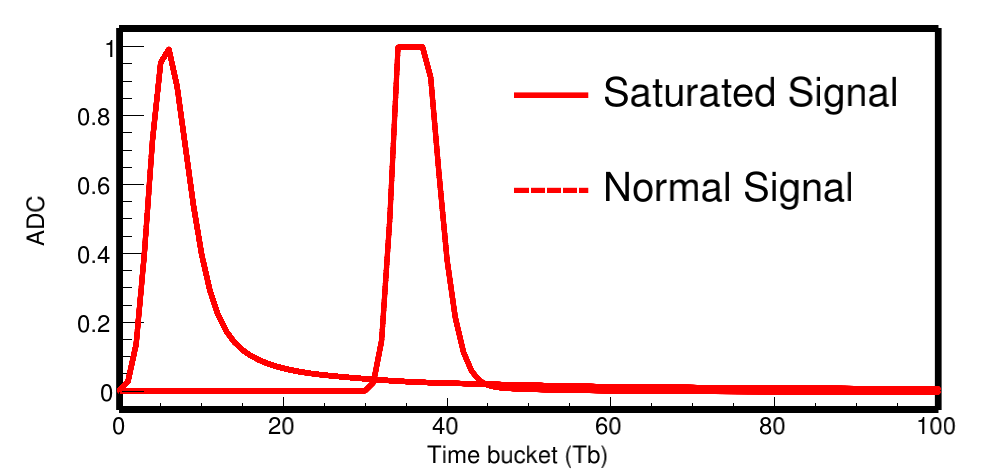
\includegraphics[width=\linewidth]{satpulse.png} 
    \caption{Standard pulse }
    \label{fig:pulseshape}
\end{figure}


\subsection{Simulating Saturation}

%Saturation of the electronics manifests itself in two different ways. Some channels are dead for the full time bucket range in an event. These channels are randomly distributed along the beam path. Though the gating grid of the TPC is closed, an un-reacted beam produces several delta electrons. The electrons emitted in directions along the magnetic field lines can physically pierce this grid and avalanche on the anode wire causing channels along the beam path to be saturated. The recovery time depends on the input charge and can take several ms to recover, killing the pad for future events. 
%Tracks depositing enough energy may saturate an electronics channel for the event shadowing tracks that may cross below. 

%From the time a channel has been saturated, no further signals can be read out. To simulate this behavior when embedding signals from Monte Carlo tracks, we must first identify when in a pad a saturating signal has occurred. Non-saturating signals have a characteristic long exponential tail where as saturated signals have no long tail and prematurely end. By applying a software pole-zero correction technique, the long tail of the non-saturated signal can be removed. In the case of saturated pules this creates a negative undershoot which we use to identify when a channel has been saturated. 

%Before embedding any MC signals into the software, the pole-zero compensation is applied to see when in time the saturation has occurred. The point in which MC signals cannot be embedded is set to 30 Tbs prior to this negative undershoot to prevent any MC signals from superimposing upon the saturated signal. Another routine identifies if a pad is ``dead" for the event and no MC signals may be embedded. 

There are several types of saturation that must be simulated or accounted for to correctly model the TPC response. They all are varying degrees of the same effect which manifest in different ways in the detector. In general all amplifiers have a finite range of output values set by a positive and negative rail (typically -12V and +12V). If the input charge into a charge sensitive pre-amplifier causes the output voltage to reach the max (or min) output voltage, the electronics is considered saturated and the response may be non-linear. The picture is complicated by the fact that there is usually an RC feedback loop which dissipates the input charge. The time in which a pre-amplifier returns to its typical linear behavior depends on the input charge and how quickly it can be dissipated \cite{akiGET}. The pad is otherwise considered dead and no further charge can be measured until the electronics recover. 
 
Due to the long high energy tail in energy loss distributions of a particle traversing matter, it is common to see pads along the track which have very high energy loss values and saturate the electronics of that pad, even for minimum ionizing tracks. Saturation in this case is infrequent and not an issue as many other clusters are not saturated. As the particle's charge gets higher, or the momentum gets lower, the mean energy loss value gets much higher and a significant fraction of pads in a track may be saturated. While earlier we outlined and algorithm to correct the saturation for the track measurement itself, saturation also affects surrounding tracks. 

As mentioned earlier the pad is dead for some time, which depends on the total input charge. For charges that are relatively at or above the threshold for saturation the pad is certainly dead for the remainder of time of the measurement; i.e. $T_{dead}$ > \SI{10}{\micro\second}. This will cause signals from other tracks passing underneath the offending track to not be measured; the saturated pad ``shadows" any future signal. In the case where two tracks are separated in time due to different polar angles, but have significant overlap in a pad-plane projection, a significant portion of the later track may be shadowed and the track itself will suffer in quality significantly. For events with high track multiplicity this causes a significant shadowing effects, in that the upward going tracks recorded at earlier times shadow the downward going tracks recorded at later times. This will change event by event and is very difficult to simulate except through a MC track embedding approach which will be discussed later. 

\begin{figure}[!htb]
\centering
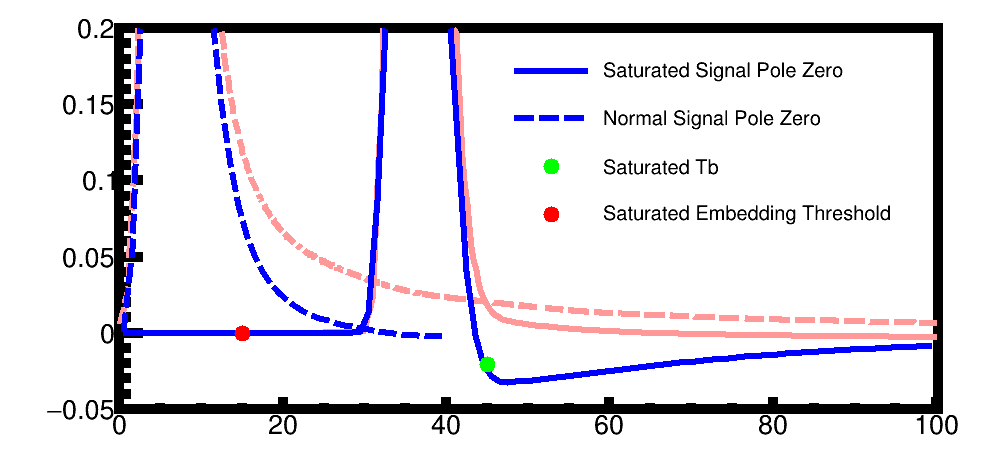
\includegraphics[width=\linewidth]{satpulsepz.png} 
\caption{Pole zero correction} 
\label{fig:pulseSatTag}
\end{figure}


In the case where the input signal is very large, the electronics can be dead for up to \SI{35}{\milli\second} \cite{akiGET}. The beam rate in the experiment was about \SI{10}{\kilo\hertz}, which corresponds to an average of \SI{10}{\micro\second} between subsequent beams. Pads can be effectively dead for several events before recovering. Due to the large charge of the beam, a large amount of very high energy electrons are produced via scattering from the beam passing through the gas. In the presence of the magnetic field the radius of curvature of most of the electrons are within several \si{cm}. Figure~\ref{fig:deltaE} shows the horizontal extent of the electrons in a top down view of the TPC. While some of the electrons can stop in the gas, a significant fraction can travel to the top and bottom of the TPC. These electron can pass through the gating grid without being blocked and either terminate on the pad or possibly deposit their charge directly in the pad. The charge induced on the pad was large enough to kill the pad for a time long enough to last until at least the next event. These pads are dead for the whole event and are randomly distributed around the beam path projection on the pad plane. 


\begin{figure}[!htb]
    \centering
    \begin{subfigure}[t]{0.49\textwidth}
        \centering
        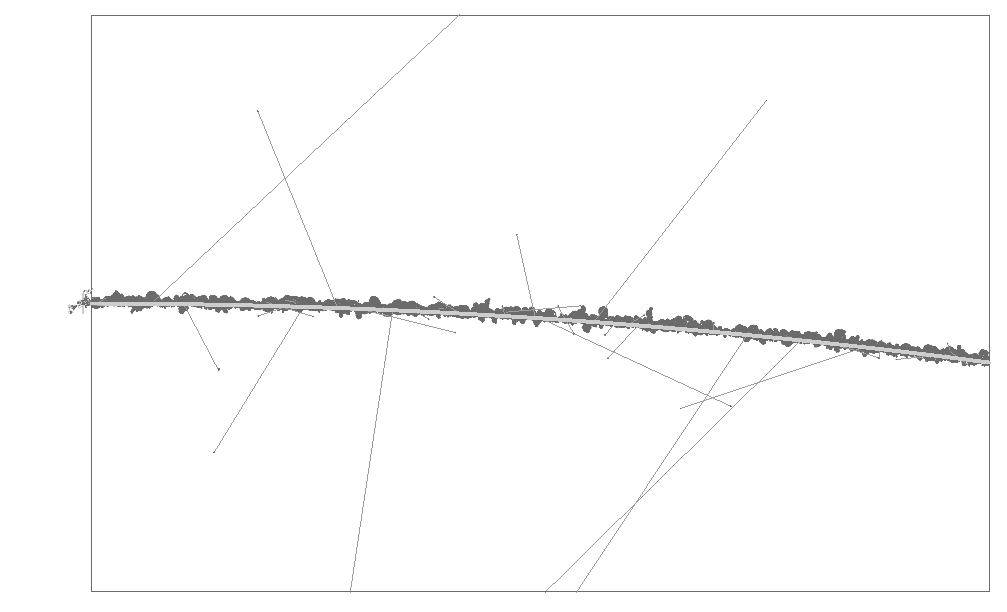
\includegraphics[width=\linewidth]{deltaE_topview_neg} 
        \caption{Top view} \label{fig:deltaE_topview}
    \end{subfigure}
    \hfill
    \begin{subfigure}[t]{0.49\textwidth}
        \centering
        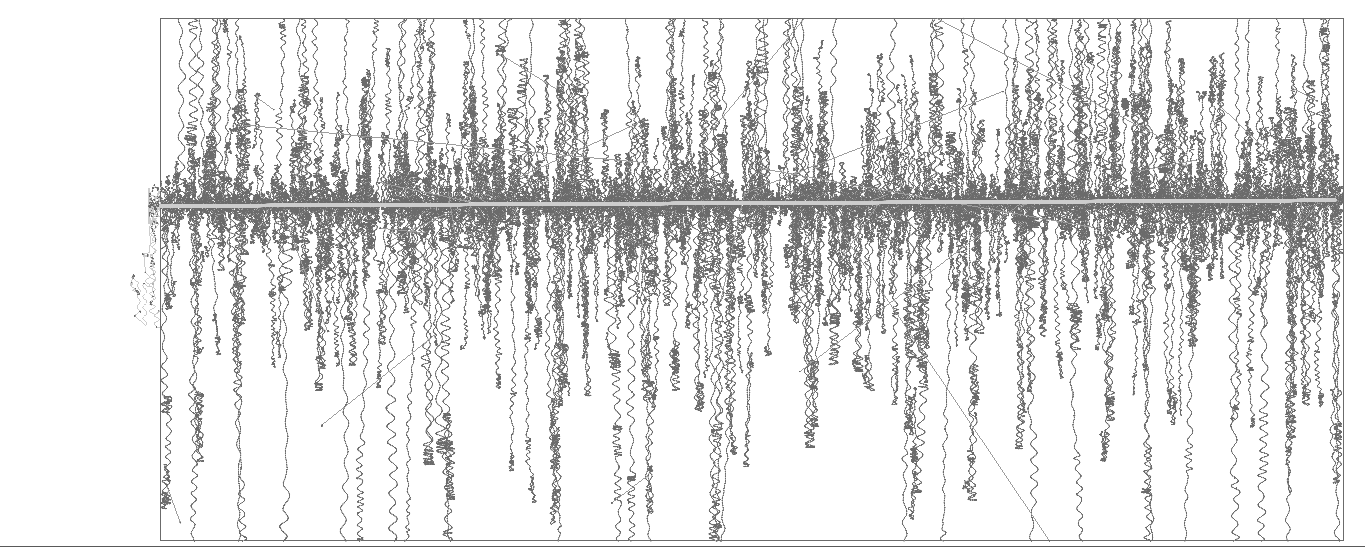
\includegraphics[width=\linewidth]{deltaE_sideview_neg} 
        \caption{Side view} \label{fig:deltaE_sideview}
    \end{subfigure}
    \caption{Geant4 simulation of ${}^{108}$Sn beam at 270 MeV/A in P10 gas. Notice the extent of the delta electrons in the vertical direction as compared to the horizontal extent. }
\label{fig:deltaE}
\end{figure}


\begin{figure}[!htb]
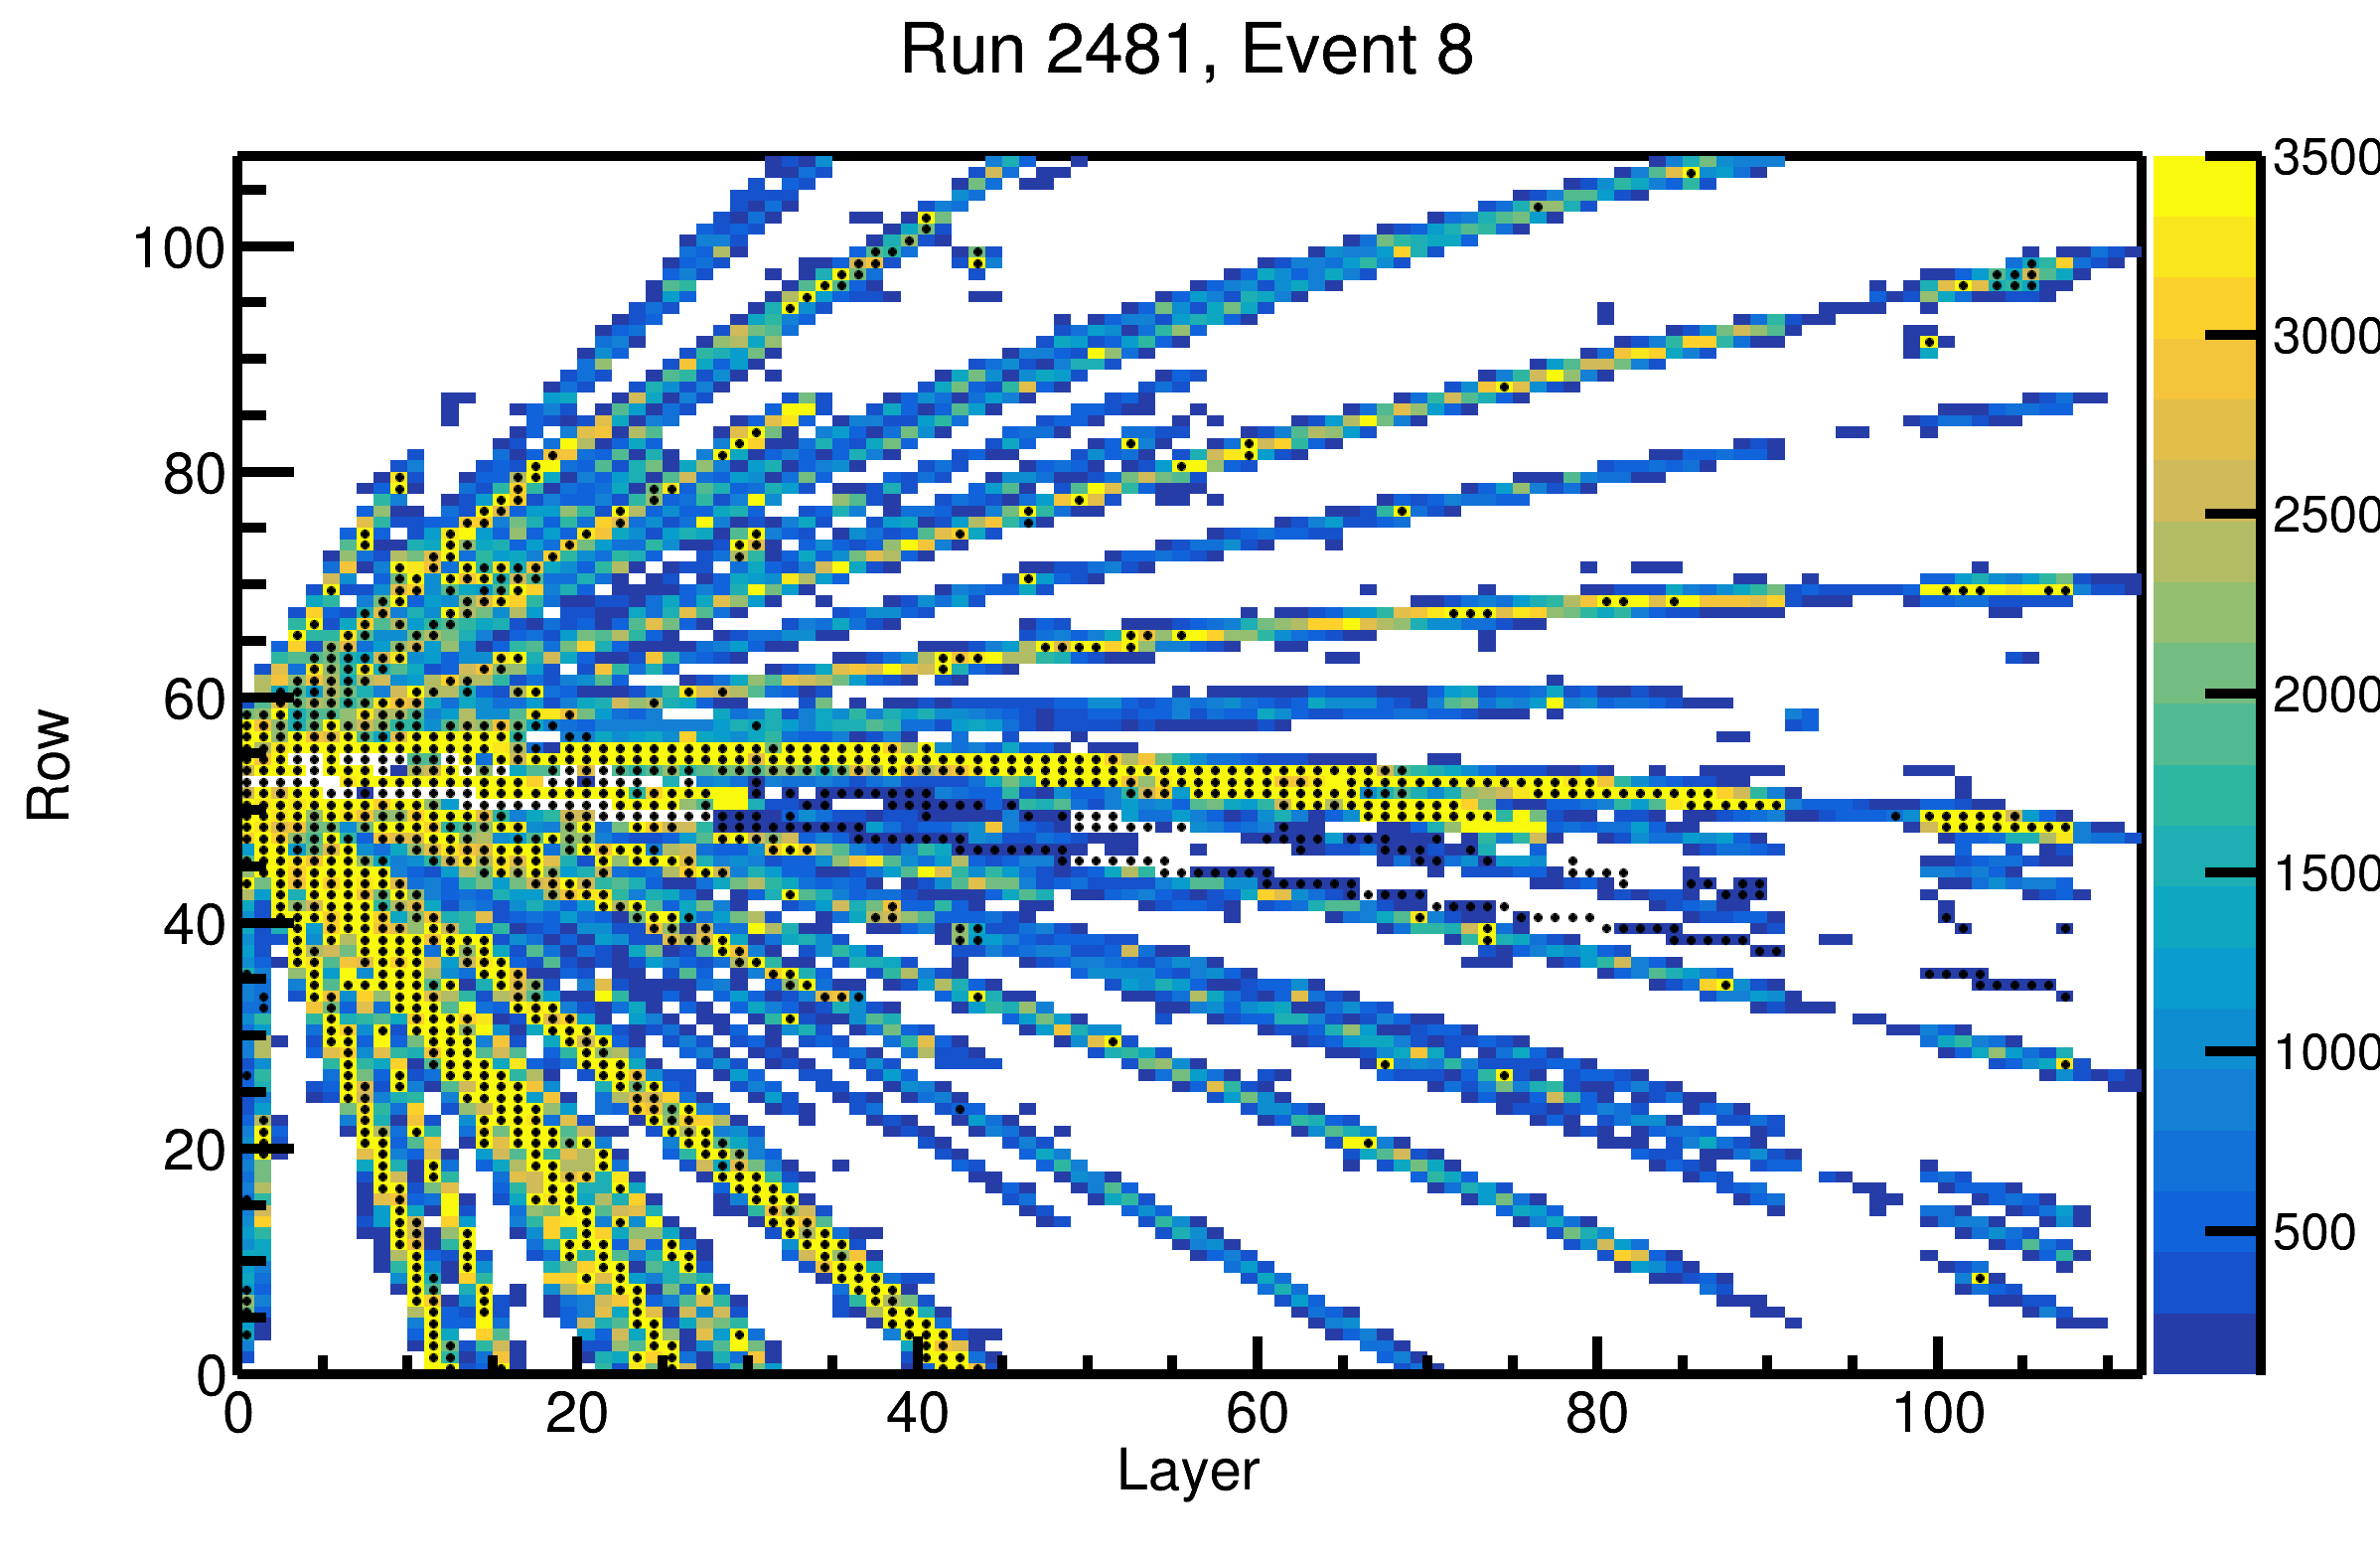
\includegraphics[width=\textwidth]{padplane_sat.png}
\caption{Tagging the saturated pads.}
\label{fig:satTag}
\end{figure}

Simulation of saturation is handled naturally by embedding MC tracks into real data, by correctly identifying when in the time bucket spectrum saturation has occurred in each pad. Once the time of saturation has been identified, no further signals are embedded as the pad is assumed to be dead. In the case a pad is dead for the whole event the time of saturation is set to the first time bucket and no signal is embedded. The characteristic signature of a saturated signal is the fast fall time of the falling edge of the pulse going quickly to zero, as opposed to the long tail of normal pulses as seen in Fig.~\ref{fig:pulseshape}. The long exponential tail can be effectively removed by a simple software technique which is similar to the electronics concept of ``pole-zero compensation". If the raw ADC value at a particular time, $i$, is represented as $f_i$, the corrected pulse which differentiates out the exponential tail, $f_i^{'}$ can be expressed as, 

\begin{equation}
f_i^{'} = \frac{-b_1\cdot f_{i-1}^{'} + a_o\cdot f_i + a_1 \cdot f_{i-1}}{b_o}
\label{eq:satpolez}
\end{equation}

where $a_o$ = .9723, $a_1$=-.9453, $b_o$=.9545, and $b_1$=-.9203. These numbers are experimentally fit to give the fastest, non-zero, correction to the tail of a normal pulse. This correction produces a negative undershoot for the saturated pulse, since there was no long exponential tail to begin with. Figure~\ref{fig:pulseshape} shows before the correction technique as the red curves, and after the technique as the blue curves for both the normal and saturated pulse. 
As the program is looking for and identifying positive peaks in the spectrum, we also calculate the corrected ADC value of that particular time bucket according to Eq.~\ref{eq:satpolez}. A peak is identified as a saturated signal if it is less than -20$\cdot G$ for more than 8 Tbs, where $G$ is the gain calibration of the pad, and the max ADC value is > $G\cdot$500 to eliminate false negative pulses which come from the gating grid subtraction in dead pads. The saturated flag is set to true and the data time bucket position of saturation is set to $t_{peak} - 5$, where $t_{peak}$ is the time bucket of the negative peak. The MC time bucket position is set to $t_{peak} - 30$ to ensure that the MC signals do not overlap the saturating data signal.

Saturation can also occur if the sum of all the pulse heights are over the max ADC threshold of 3500 ADC. This is because the fall time of the pre-amplifier circuit is much longer than the time bucket window and pulses are allowed to pile up. While pads that saturate via this method still are identified through the same algorithm described above, nothing is done in the MC class to take this into account when embedding signals. We assume this method of saturation is a higher order correction and the current algorithm approximates most of the saturation effects. Figure~\ref{fig:satTag} shows the tagging algorithm for an event in the TPC. The max ADC values in a given pad are colored and the black dots are pads tagged as saturated. Some pads appear to be below 3500 ADC, but upon further inspection they satisfy the sum of all the signals causes saturation though the max ADC never goes over 3500. 

Dead pads are identified earlier in the software in the STCore.cc class. A dead pad is classified as having a r.m.s. value  < 50 ADC and a max ADC < 50. The saturated flag is set to true, and the time bucket position of saturation in both the data and MC are set to the first time bucket. 


%maybe simple pream fig
%maybe example from aki paper about times
%maybe 

%Add figure showing saturated time bucket spectra with location of saturation identified and with pulse shape from embedding I would like to add and how it blocks it.
%Add Figure with 2D pad plane response with and without saturation flag


\section{Monte Carlo Track Embedding}
 The TPC monte carlo simulation was built upon Geant4, including the dimensions, materials, and gas composition. Several classes were built to simulate the operations of a Time Projection Chamber (TPC). This included the drift properties of electrons, avalanche process, and electronics response to input signals. Combined, these classes simulate the response of the TPC to any input MC track and can be directly input into the \spirit TPC software reconstruction algorithm. 

While the goal of these tasks are to simulate important properties of a TPC, there are several effects which cannot be easily simulated. Several examples are biases due to triggering detectors (preferential selection of a reaction plane), saturation effects in the electronics, track multiplicity, and several other systematic sources common to all experiments. Simulating each issue individually would be impractical and time consuming, if not impossible. By embedding monte carlo tracks into experimental data -- and propagating through the tracking and reconstruction algorithm -- one can account for all sources these type of sources with a monte carlo type approach.


Track embedding is the process of taking a simulated MC track from Geant4 and embedding its response into a real data event. After reconstructing this new embedded event we match the input MC track to its corresponding final reconstructed track.  By doing so we can evaluate the response of the entire TPC system to any given input value. The TPC system is composed of three major components, each which can introduce errors and or biases; the software, the detector, and the experimental setup.  

As discussed in Section~\ref{sec:software}, the software is composed of several task, each which introduce errors through assumptions made in the tracking algorithm. The detector system itself introduces errors related to the physical measurement itself. By modeling the TPC, and its materials, the a Geant4 simulation provides an accurate description of interactions of a particles traversing the materials of the TPC. 

% Evaluating the errors introduced by the software is the most straight forward exercise; let the software routine process an input and measure the result. Understanding the physical measurement requires modeling the physics involved in the theory and operations of TPCs and the electronics.
 
 % The experimental setup itself is quite large and complex, several ancillary detectors such as the Kyoto multiplicity array, Krakow veto array, Active veto array, beam identification detectors, etc. Even if a full accurate model could be constructed the complex trigger logic of the DAQ system would be impossible to model. If we notice that the biases and errors of the entire experimental setup is contained in the measured experimental data. Therefore, by inputting the MC data into a real experimental event (and measuring the output of that MC track) we can estimate the errors of the experimental setup. 
Before begging the detailed description of the embedding software, it is worth noting that the MC embedding was analyzed as a separate data set from the published data to avoid any issue of MC embedded tracks making it into the final published data. 

The detailed flow diagram of the software implementation of embedding is shown in Fig.~\ref{fig:flow}. 







%\begin{sidewaysfigure}[H]
%\centering
%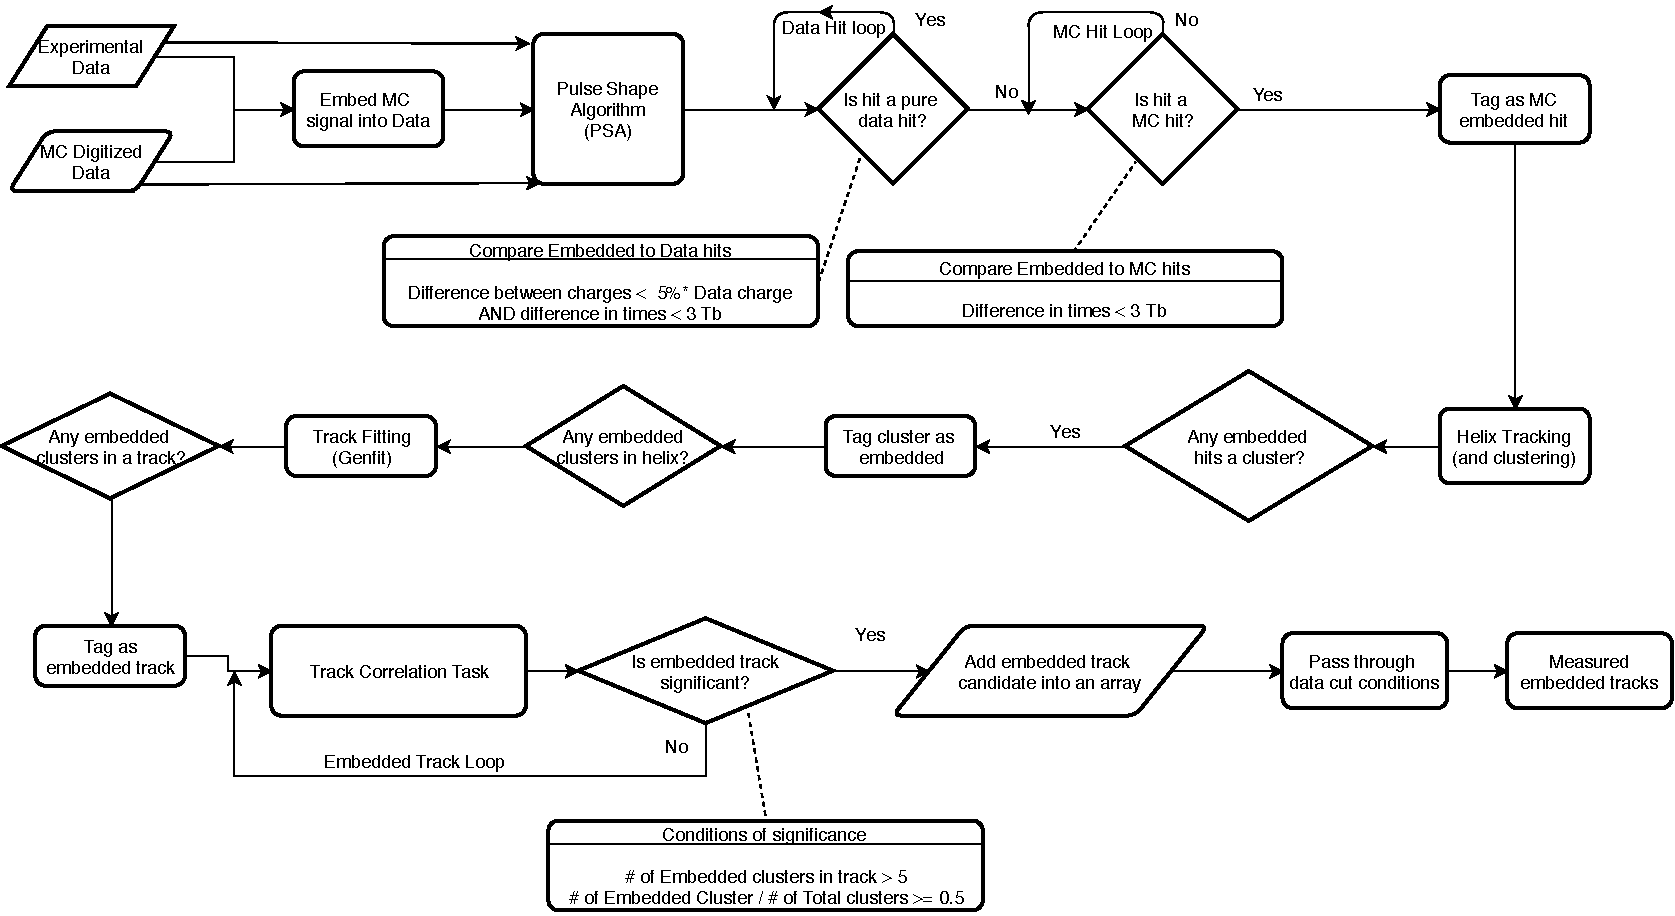
\includegraphics[width=\textwidth]{FlowEmbedding.pdf}
%\caption{Flow of embedding implementation in the software.}
%\label{fig:flow}
%\end{sidewaysfigure}


%\clearpage
%\pagestyle{lscape} % first clear the page and change the pagestyle
%\begin{landscape}
% your landscape table(s) or figure(s) here
%CONSIDER ROTATING THIS FIGURE IF ALLOWED
\begin{figure}[H]
\centering
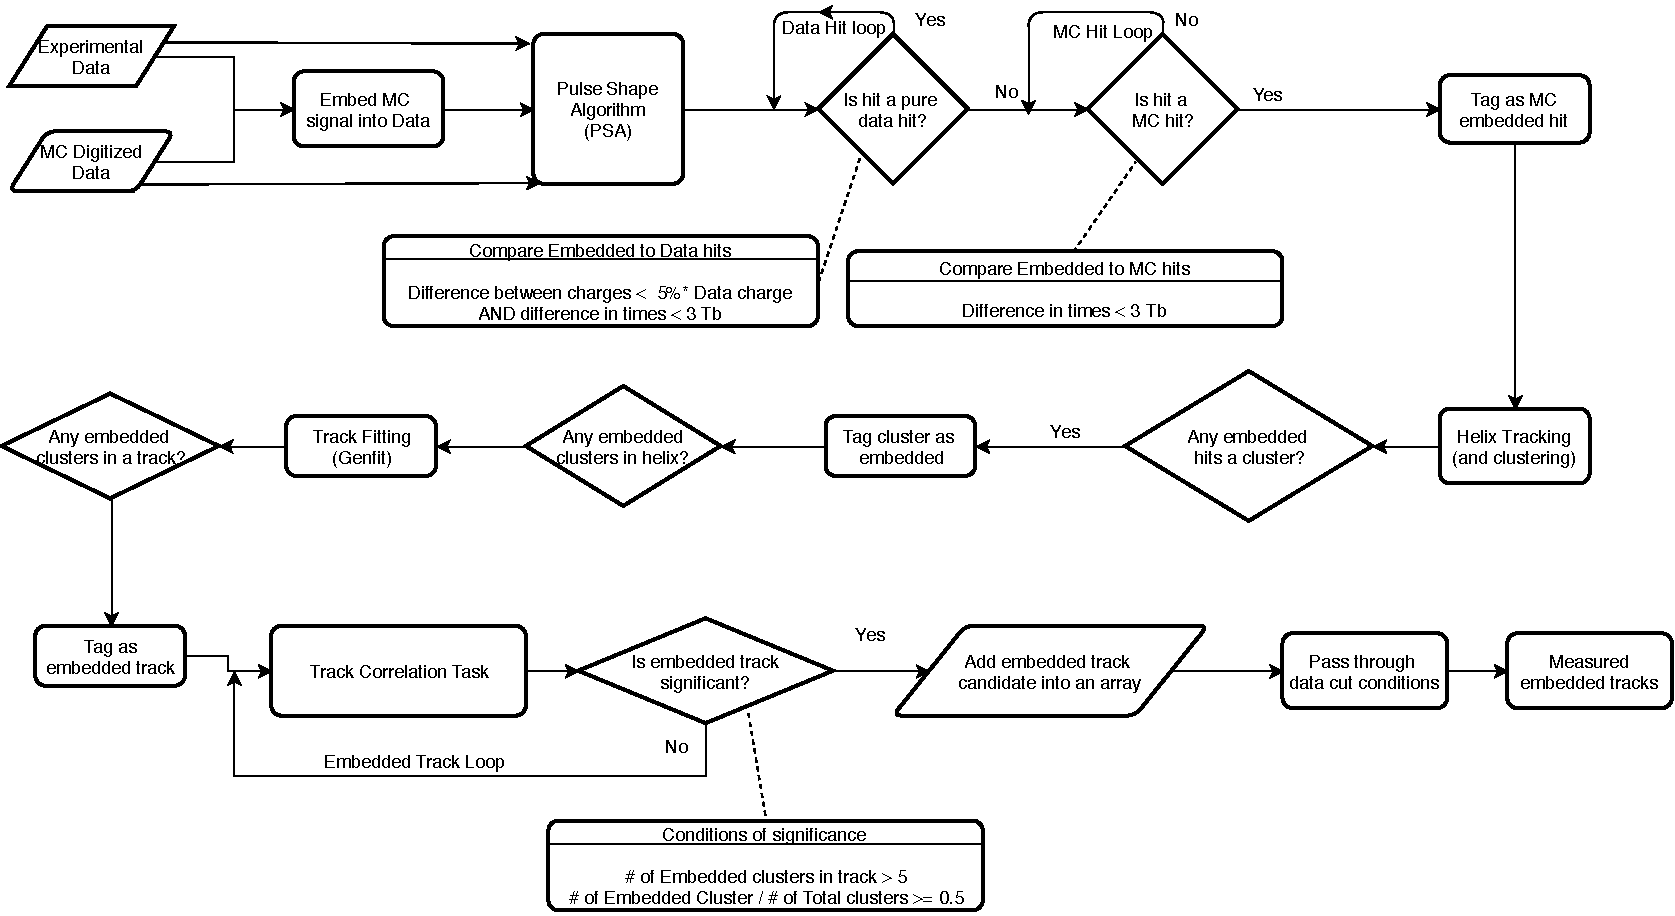
\includegraphics[width=\textwidth]{FlowEmbedding.pdf}
\caption{Flow of embedding implementation in the software.}
\label{fig:flow}
\end{figure}

%\end{landscape}
%\pagestyle{plain}

\begin{figure}[!htb]
    \centering
    \begin{subfigure}[t]{0.49\textwidth}
        \centering
        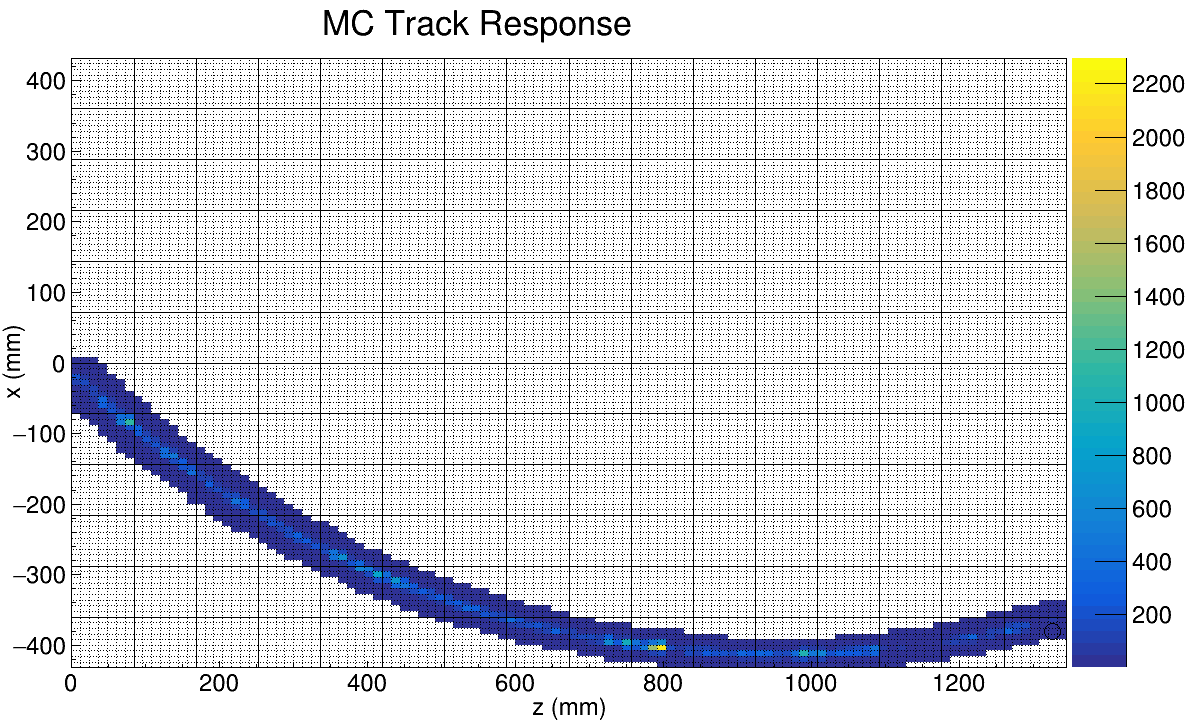
\includegraphics[width=\linewidth]{mcresponse.png}
        \caption{200 MeV/c $\pi^-$ MC digitized track} \label{fig:mcevent}
    \end{subfigure}
    \hfill
    \begin{subfigure}[t]{.49\textwidth}
        \centering
        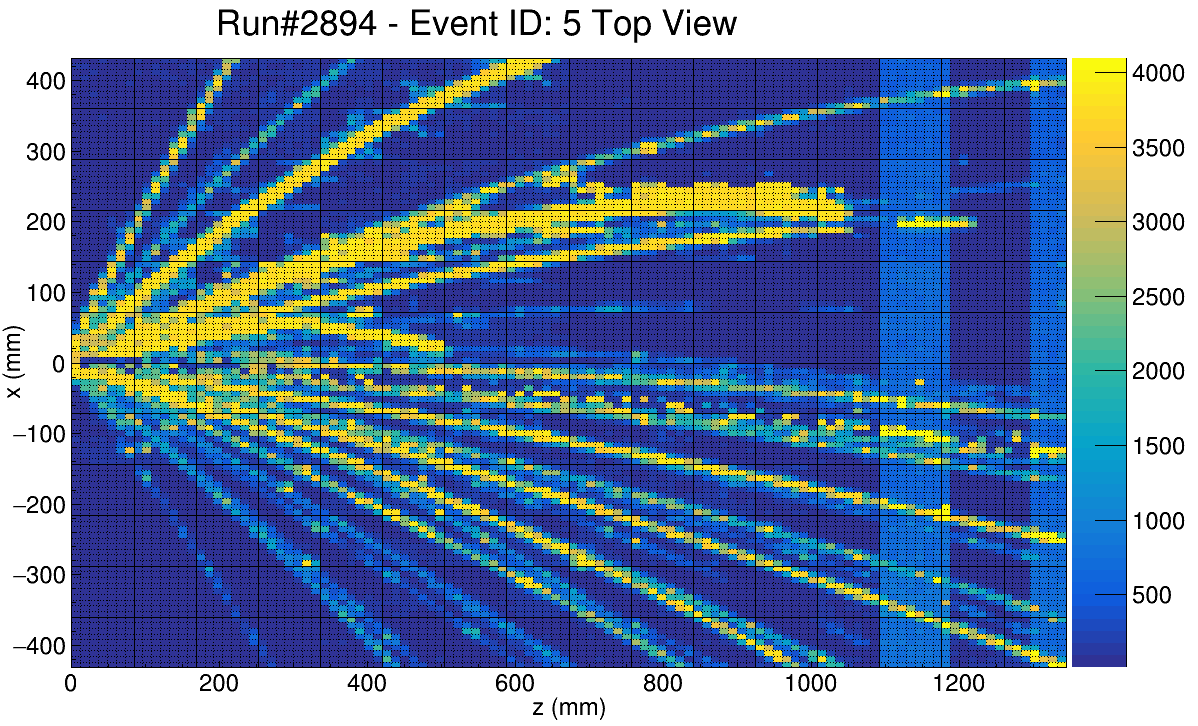
\includegraphics[width=\linewidth]{event5.png} 
        \caption{Experimental data event.} \label{fig:dataevent}
    \end{subfigure}
    \caption{A 200 MeV/c $\pi^-$ embedded into a nuclear collision type event. The embedded track identified by the software is highlighted by the solid green line. }

\label{fig:embedtrack}
\end{figure}



\begin{figure}[!htb]
    \centering
    \begin{subfigure}[t]{0.49\textwidth}
        \centering
        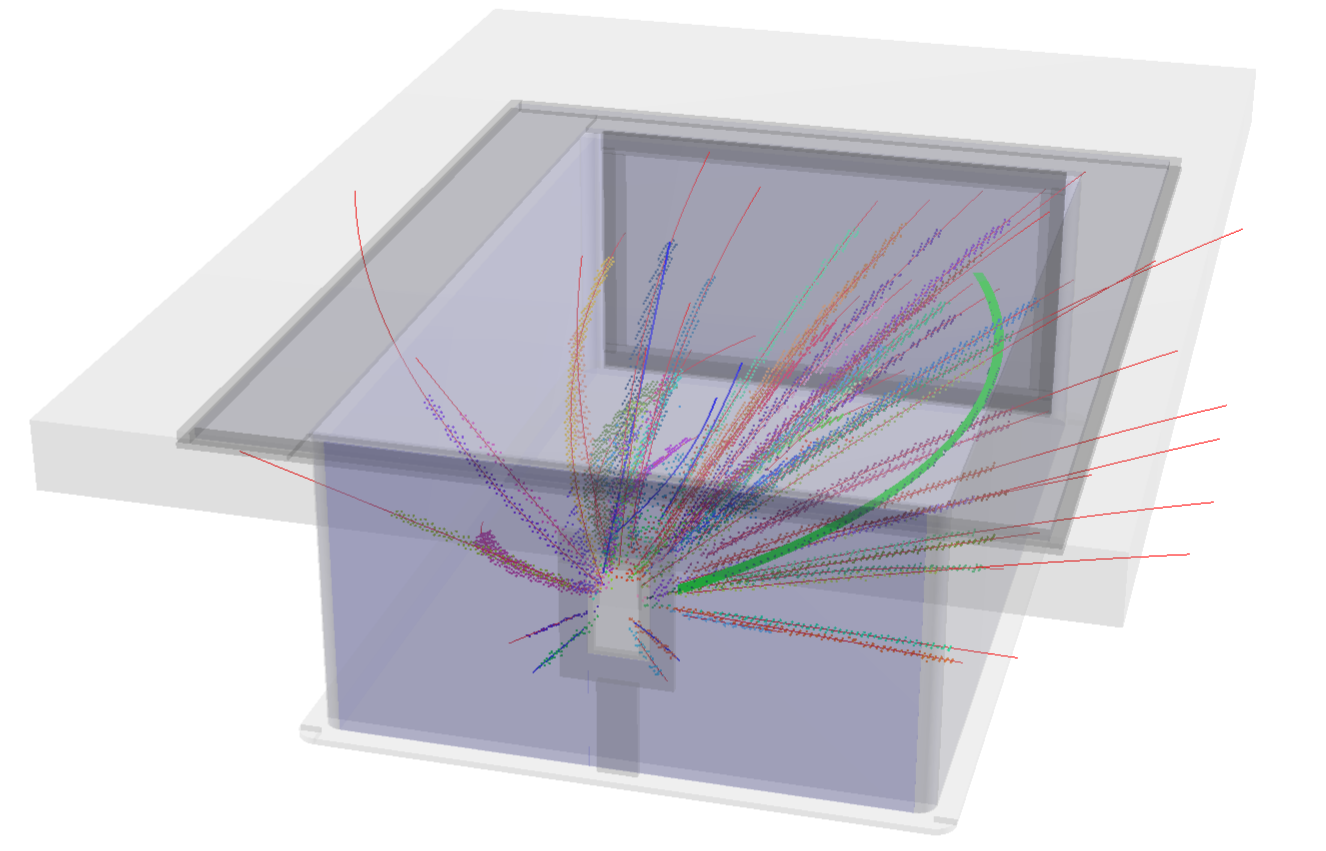
\includegraphics[width=\linewidth]{perspective_embed}
        \caption{Generic} \label{fig:persEmbed}
    \end{subfigure}
    \hfill
    \begin{subfigure}[t]{.3\textwidth}
        \centering
        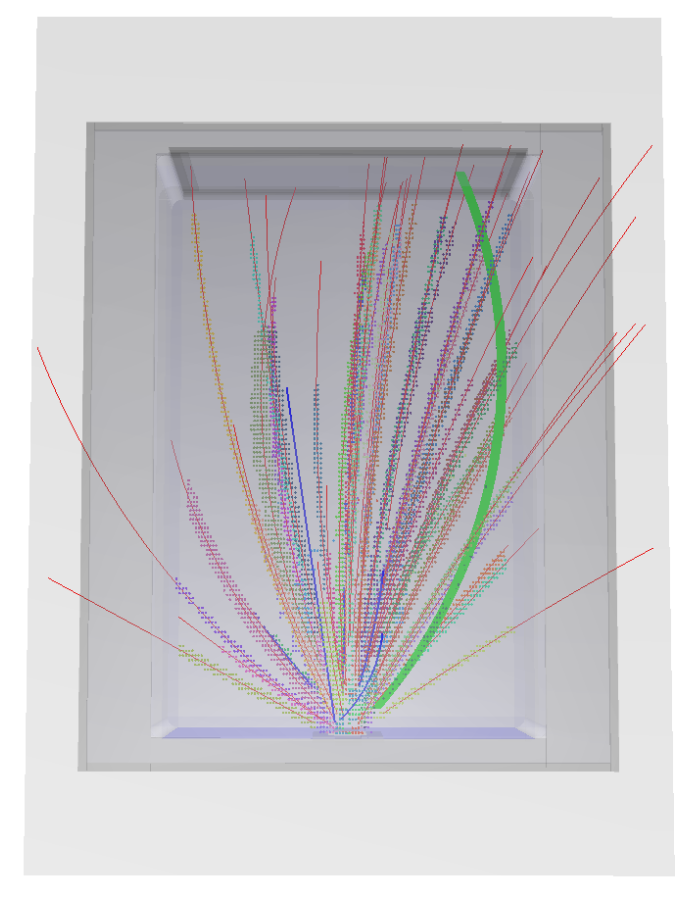
\includegraphics[width=\linewidth]{top_embed} 
        \caption{Competitors} \label{fig:topEmbed}
    \end{subfigure}
     \hfill
    \begin{subfigure}[t]{\textwidth}
        \centering
        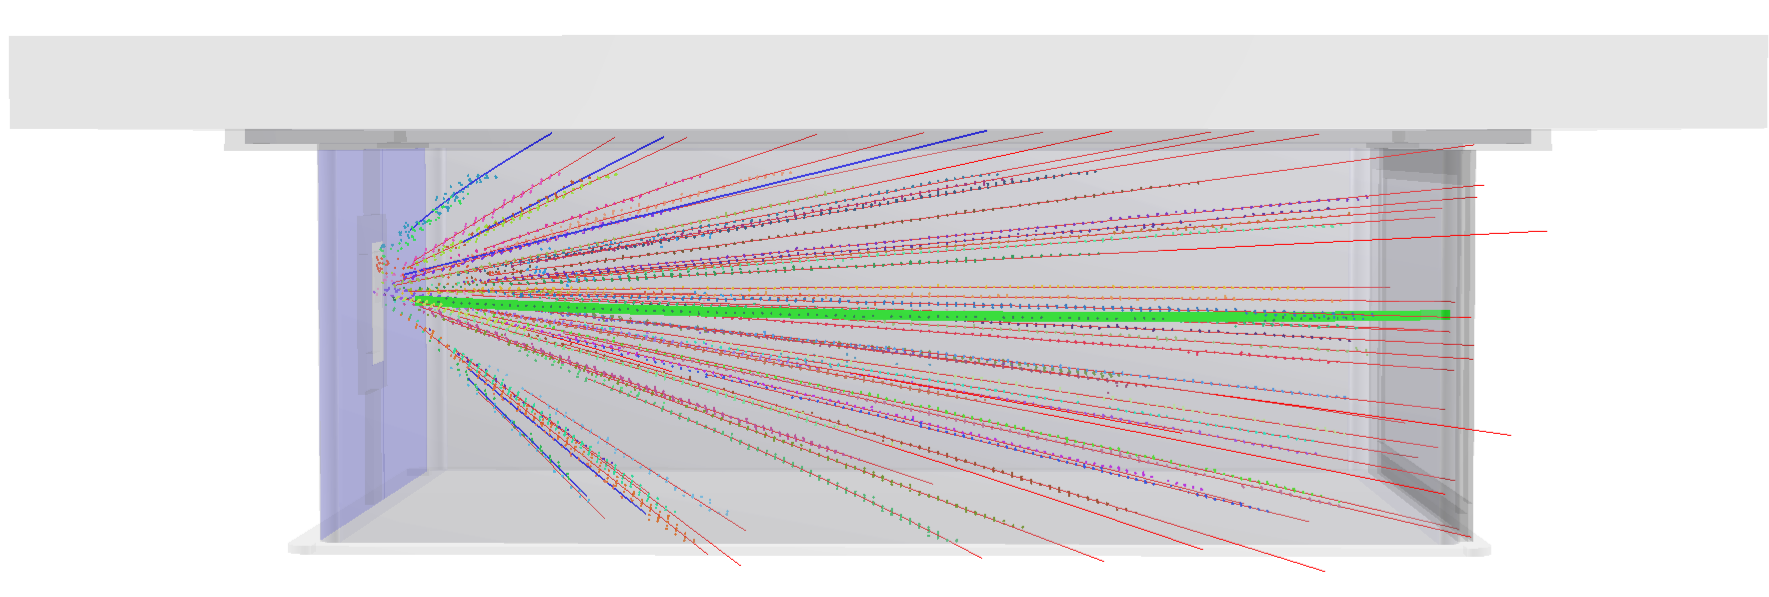
\includegraphics[width=\linewidth]{side_embed} 
        \caption{Competitors} \label{fig:sideEmbed}
    \end{subfigure}
    \caption{A 200 MeV/c $\pi^-$ embedded into a nuclear collision type event. The embedded track identified by the software is highlighted by the solid green line. }

\label{fig:embedtrack}
\end{figure}



Once the MC simulation of a track response in the TPC is created, we directly embed the MC signals into data by superimposing the MC signals into the data time bucket spectrum, pad-by-pad. We will refer to this superimposed data as ``embedded data", only the MC signals as ``MC data", and data only containing the experimental signals as ``experimental data". The three set of data are each independently analyzed by the PSA algorithm, Section~\ref{sec:psa}, finding the hits in each data set. Part of the PSA task is to identify which hits in the embedded data are MC hits and which are from the original data. Once identified the embedded hits can be tagged and tracked through the entire software.

 By comparing the hits identified in the embedded set against the experimental data set we can first identify which embedded hits belong to the original experimental hit subset. For hits to match, they must satisfy two criteria; $\left|(Q_{\mathrm{Data}} - Q_{\mathrm{Embed} })/Q_{\mathrm{Data}}\right| < .05$ and $\left|t_{\mathrm{Embed} } - t_{\mathrm{Data} }\right| < 3$ where $Q$ and $t$ represent the charge and time of the hit respectively. We then remove these hits in the embedded data set which satisfy the conditions of experimental data hits. 

The surviving hits are then compared with the MC hit data set, where the criteria for a matching MC hit is, $\left|t_{\mathrm{Embed} } - t_{\mathrm{MC} }\right| < 3$.  We do not require a matching criteria for the charge values since the pions we wish to study induce small signals relative to most of the particles producing signals in the experimental data as not to bias the charge values in the embedded data.  Since we removed almost all of the experimental hits in the first step, requiring only a time bucket cut in the second comparison is sufficient to tag the embedded MC hits. Each embedded hit that passes both criteria is tagged as an MC embedded hit. From here, the embedded data is treated as if it were real data passing through all the software algorithms as we use in the real data analysis. If a helix track has one hit that is embedded it will be tagged as embedded. Hits in a helix track are then clustered; if a cluster contains one embedded hit it is itself tagged as an embedded cluster. If a track that is reconstructed contains any embedded clusters, it is an embedded track.  

The goal of this na\"ive tagging is to preserve all the information of where the embedded hits, clusters, and tracks have gone. The  job of the embedded correlation task is to identify which of the embedded tracks are candidates for the original input track. Several things may happen along the process of embedding. A track could break up, lose or share its charge with and adjacent track, or maybe not be identified for other reasons. For the embedded track to be a candidate it must satisfy two conditions, $N_{sat} > 5$ and $N_{\mathrm{sat}}/N_{\mathrm{Total}} \geq .5$, where $N_{\mathrm{sat}}$ is the number of saturated clusters in a track and $N_{\mathrm{Total}}$ is the number of total clusters. The first criteria is a simple minimum cut where to ensure there exists an embedded track and the second criteria is the strongest cut ensuring the track has at least half of its clusters coming from embedded MC signals. The set of tracks which satisfy both conditions are saved into an array of tracks which the user can use to study efficiency or track splitting. 

In the case of efficiency analysis the user must select what they believe to be the track which most represents the original track. In this thesis, the track with the minimum distance to vertex is identified as the correct track. Though track splitting may occur, typically the split track has a distance to vertex which is very large and cut out from the analysis. The details of the efficiency analysis will be described later. 



\subsection{MC and Data Comparison}

\begin{figure}[!hbt]
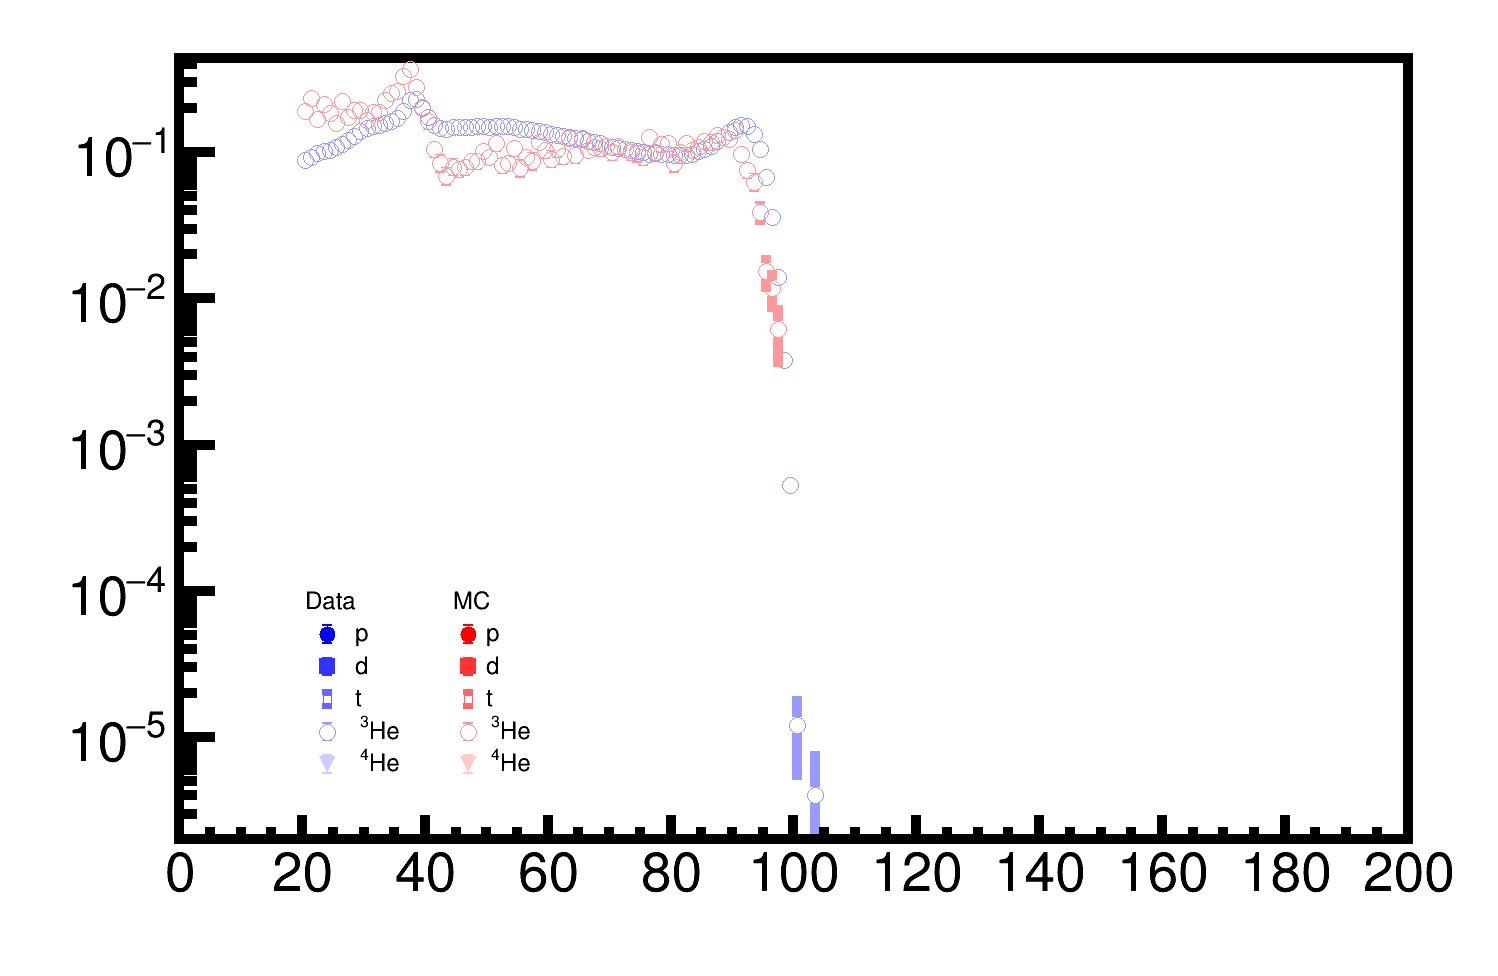
\includegraphics[width=\linewidth]{numcluster.png}
\caption{Comparison of MC to data.}
\label{fig:clustcomp}
\end{figure}


\begin{figure}[!hbt]
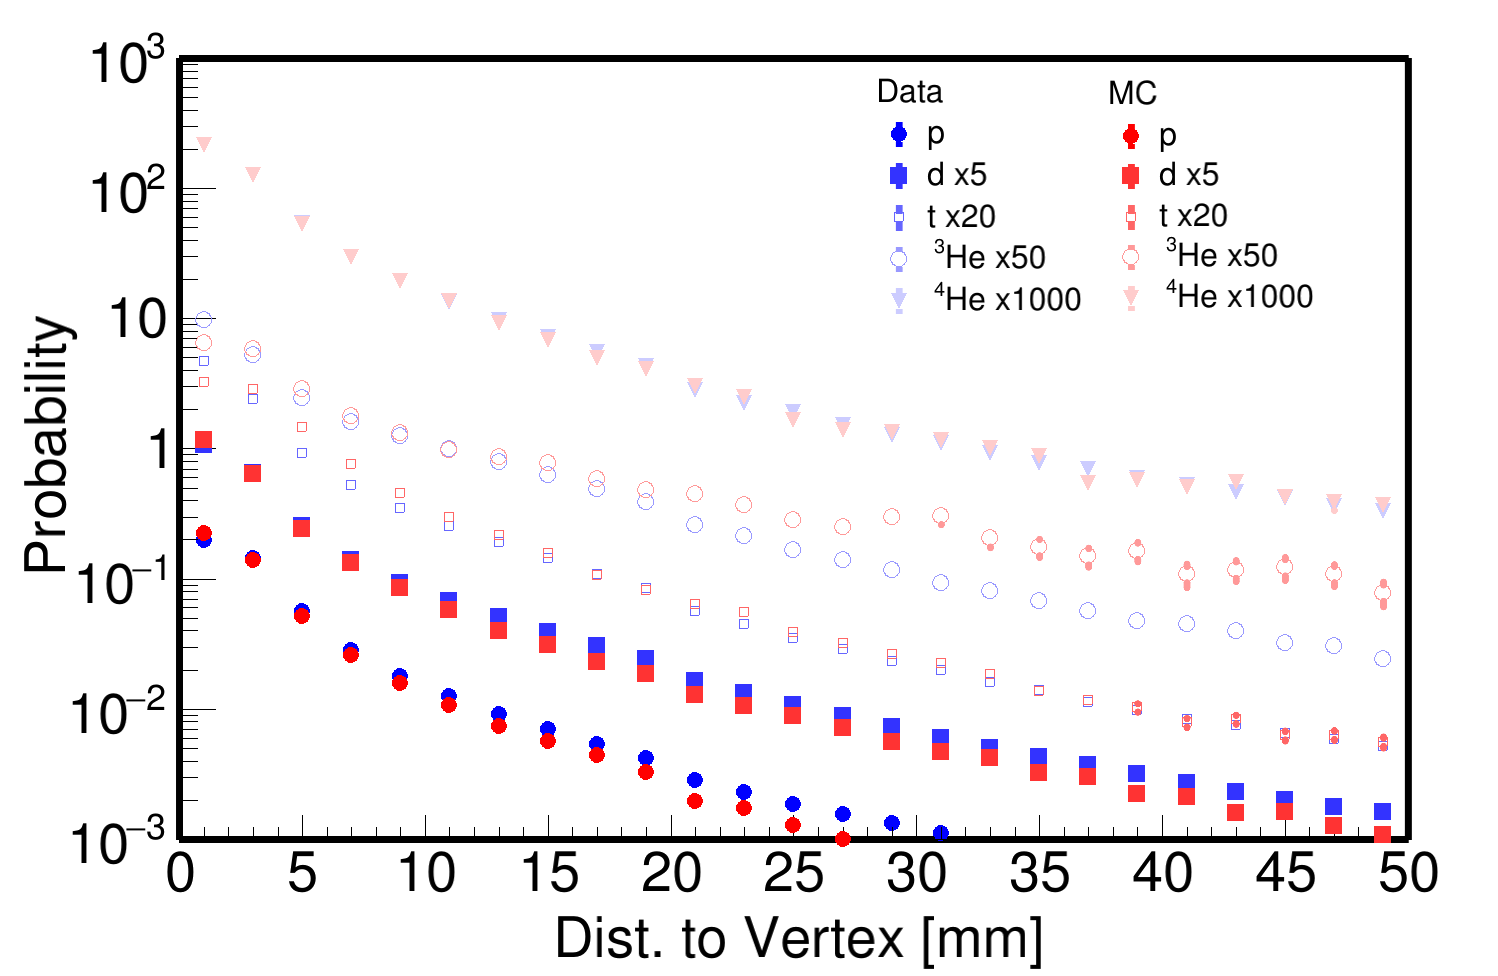
\includegraphics[width=\linewidth]{poca.png}
\caption{Comparison of MC to data.}
\label{fig:pocacomp}
\end{figure}


Add Figure of Pad response function for pion,proton.... for MC vs Data vs angles...
Add Figure of Number of clusters of MC vs Data
Add Figure of dEdx MC vs Data
Add Figure of Momentum resolution MC vs Data
Add Figure of track residuals? MC vs data?


\section{Aligning TPC}

\section{CoBo timing correction}

\section{Efficiency Corrections}
Add Figures of efficiency vs angles in TPC polar angle plot for pions


Since the \spirit TPC is a fixed target experiment it's angular coverage is certainly not 4$\pi$. Because the target is several cm away from the widow of the field cage the geometric acceptance is not even 2$\pi$. The rectangular design complicates the calculation of the geometric acceptance, or the efficiency.


